% PVLDB (acmart-based) version. Migrated from IEEEtran.
\documentclass[sigconf, nonacm, review]{acmart}

%% packages and macros ported from working draft
\usepackage{tikz}
\usetikzlibrary{arrows.meta,positioning,shapes.geometric,backgrounds,fit}
\usepackage{algorithm}
\usepackage{algpseudocode}
\usepackage{tabularx}
\usepackage{enumitem}
\setlist[itemize]{leftmargin=*}
\setlist[enumerate]{leftmargin=*}
\usepackage{pgfplots}
\usepgfplotslibrary{groupplots}
\pgfplotsset{compat=1.18}
\usepackage{colortbl}
\definecolor{letherow}{RGB}{223,237,245}
\definecolor{good}{RGB}{0,158,115}\definecolor{leakc}{RGB}{213,94,0}\newcommand{\cmark}{\tikz[scale=0.14,baseline=-0.1ex]{\draw[line width=0.9pt,good!80!black,line cap=round,line join=round](0,0.5)--(0.42,0)--(1.25,1.0);}}
\newcommand{\xmark}{\tikz[scale=0.14,baseline=-0.1ex]{\draw[line width=0.9pt,leakc,line cap=round](0,0)--(1.05,1.05) (0,1.05)--(1.05,0);}}
\newcommand{\Nout}{N_{\mathrm{out}}}
\newcommand{\Nin}{N_{\mathrm{in}}}
\newcommand{\rev}{\mathsf{revoke}}

%% VLDB paper and issue block
\newcommand\vldbdoi{XX.XX/XXX.XX}
\newcommand\vldbpages{XXX-XXX}
\newcommand\vldbvolume{20}
\newcommand\vldbissue{1}
\newcommand\vldbyear{2027}
\newcommand\vldbauthors{\authors}
\newcommand\vldbtitle{\shorttitle}
\newcommand\vldbavailabilityurl{https://anonymous.4open.science/r/lethe/}
\newcommand\vldbpagestyle{plain}
\newif\ifextended\extendedtrue % build the GitHub extended version; set \extendedfalse for the 12-page submission
\AtBeginDocument{\newtheorem{assumption}[theorem]{Assumption}\newtheorem{remark}[theorem]{Remark}}

\usepackage{cuted}
\begin{document}
\title[Zombie Vectors]{Laying Zombie Vectors to Rest:\\Per-View Erasure in Graph Indexes}
\author{Yizheng Zhao}
\affiliation{%
  \department{State Key Laboratory of Novel Software Technology}
  \institution{Nanjing University, China}
  %\city{Nanjing}
  %\country{China}
}
\email{zhaoyz@nju.edu.cn}
\author{Wanjing Ren}
\affiliation{%
  \department{State Key Laboratory of Novel Software Technology}
  \institution{Nanjing University, China}
  %\city{Nanjing}
  %\country{China}
}
\email{renwj@smail.nju.edu.cn}

\begin{abstract}
Revoking a user's access to a vector should make it vanish from that user's
results. In a shared graph index, the standard for high-recall approximate
nearest neighbor (ANN) search, it does not. The vector cannot simply be
deleted: other users still need it, and true deletion demands costly
neighborhood repair, so systems merely flag it. It stays in the graph,
steering the revoked user's search, and remains byte-recoverable from memory
and snapshots. We call these \emph{zombie vectors}. Every existing remedy is global: leaving the vector lets it keep routing, removing or shredding it erases it for every user at once, and rebuilding per revocation is prohibitively expensive. Erasure is therefore not a structural delete but a per-view property of traversal: after revocation the
index must behave, in both results and routing, as if the vector had never
entered the revoked user's view, while staying unchanged for everyone else.
This guarantee, \emph{per-view erasure}, spans six independent axes
(Results, Routing, Physical, Immediate, Verifiable, View-scope); Tombstone,
Physical-delete, Periodic-rebuild, and cryptographic shredding each violate
at least two. We present \textsc{Lethe}, an index and query-processing design
that satisfies all six: revocation-aware traversal with a bypass overlay,
shared across principals with the same view, that keeps a revoked vector's authorized neighbors
reachable; cryptographic shredding for global physical
erasure; and an append-only erasure log. Across clinical, legal, web, and
standard ANN benchmarks, \textsc{Lethe} drives per-view leakage to near zero,
holds recall near an oracle per-view rebuild, and
erases immediately at far lower memory than per-user indexes, scaling to a
billion vectors. Erasure belongs where queries are answered, not where data is
stored.
\end{abstract}

\maketitle

%%% do not modify the following VLDB block %%
%%% VLDB block start %%%
\pagestyle{\vldbpagestyle}
\begingroup\small\noindent\raggedright\textbf{PVLDB Reference Format:}\\
\vldbauthors. \vldbtitle. PVLDB, \vldbvolume(\vldbissue): \vldbpages, \vldbyear.\href{https://doi.org/\vldbdoi}{doi:\vldbdoi}
\endgroup
\begingroup
\renewcommand\thefootnote{}\footnote{\noindent
This work is licensed under the Creative Commons BY-NC-ND 4.0 International License. Visit \url{https://creativecommons.org/licenses/by-nc-nd/4.0/} to view a copy of this license. For any use beyond those covered by this license, obtain permission by emailing \href{mailto:info@vldb.org}{info@vldb.org}. Copyright is held by the owner/author(s). Publication rights licensed to the VLDB Endowment. \\
\raggedright Proceedings of the VLDB Endowment, Vol. \vldbvolume, No. \vldbissue\ %
ISSN 2150-8097. \\
\href{https://doi.org/\vldbdoi}{doi:\vldbdoi} \\
}\addtocounter{footnote}{-1}\endgroup
%%% VLDB block end %%%

%%% do not modify the following VLDB block %%
%%% VLDB block start %%%
\ifdefempty{\vldbavailabilityurl}{}{
\vspace{.3cm}
\begingroup\small\noindent\raggedright\textbf{PVLDB Artifact Availability:}\\
The source code, data, and/or other artifacts have been made available at \textcolor{blue}{\url{\vldbavailabilityurl}}.
\endgroup
}
%%% VLDB block end %%%

\section{Introduction}
\label{sec:intro}
A single vector index increasingly answers similarity-search queries for
many users at once, with access governed by per-user or per-role
permissions~\cite{DBLP:journals/corr/abs-2505-01538,DBLP:journals/corr/abs-2401-07119}.
A hospital assistant retrieves over a shared embedding of patient notes,
but a clinician reassigned off a case must lose access to those notes; an
enterprise copilot retrieves over one corporate index, but a reclassified
document must disappear for users below its new clearance; a data subject
invokes the right to be forgotten~\cite{GDPR16}, and their vector must
stop reaching anyone. In each case, access to a vector is \emph{revoked}
for some users while the vector itself must remain for others. The system cannot
simply delete~it.

Graph-based indexes such as HNSW~\cite{DBLP:journals/pami/MalkovY20} and
DiskANN~\cite{DBLP:conf/nips/SubramanyaDSKK19} are the standard for
high-recall similarity search and the backbone of production vector
databases~\cite{DBLP:conf/sigmod/WangYGJXLWGLXYY21,DBLP:journals/pvldb/GuoLXYYLCXLLCQW22}.
They are also where revocation goes wrong. Deleting a node from a
navigable graph is expensive: its in-neighbors must be re-patched so that
traversal still reaches the rest of the graph, at a cost that grows with
the node's in-degree~\cite{DBLP:journals/corr/abs-2105-09613}. To avoid
paying this cost on every deletion, production systems \emph{tombstone}:
they mark a vector deleted, filter it from results, and defer the
neighborhood repair to a periodic consolidation
pass~\cite{DBLP:journals/corr/abs-2105-09613}.
A tombstoned vector therefore (i) stays physically present and
byte-recoverable, in memory and in serialized snapshots, and (ii) keeps
serving as a routing waypoint that steers traversal, including the
traversal that answers a revoked user's query. We call a revoked vector
that still routes a \emph{zombie vector}: dead to the access policy, yet
still choosing the living results. The effect is not marginal: on a clustered index, revoking by semantic cluster can shift more than one in six of a user's authorized top-10 answers away from an oracle per-view rebuild (\S\ref{sec:phenomenon}).

Why has this gone unaddressed? Work on forgetting data splits along two
layers that both skip the index. Secure deletion erases bytes from the
storage medium~\cite{DBLP:conf/sp/ReardonBC13} but not the derived
structural copies an index keeps; machine unlearning removes a datum's
influence from a trained
model~\cite{DBLP:conf/sp/BourtouleCCJTZL21,DBLP:conf/sp/CaoY15,DBLP:conf/nips/GinartGVZ19},
but a vector index has no model to retrain. Between them sits the index
structure itself, and it is empty. Vector-index research treats deletion as
a freshness problem, removing vectors globally to protect
recall~\cite{DBLP:conf/sosp/XuLLXCZLYYYCY23,DBLP:journals/corr/abs-2502-13826,DBLP:journals/corr/abs-2411-00970,DBLP:journals/corr/abs-2407-07871,DBLP:journals/corr/abs-2206-10839,DBLP:journals/pvldb/YuLGXLZSZLY25}
or characterizing deletion accuracy without security or per-user
scope~\cite{DBLP:journals/corr/abs-2512-06200}; cryptographic shredding
discards a vector's key~\cite{DBLP:journals/corr/abs-2601-07004} but
globally, leaving the node routing; and a relational notion of erasure under
dependencies~\cite{DBLP:journals/pvldb/ChakrabortyKMNNPSV25} does not model
graph traversal. No existing method erases a vector from one view while
leaving it intact for the rest.

Our starting point is a reframing: erasing a vector from a graph index is
not removing its bytes, it is removing its influence on traversal, and
that influence is exactly what Tombstone and cryptographic shredding leave
behind. In a shared index this influence is per-view, and removing it is what we
call \emph{per-view erasure}: after revocation the index must behave, in
both its results and routing, as if the vector had never entered the
revoked user's view, while remaining unchanged for every other view.

Against this definition we
characterize prior methods on six axes (\emph{Results}, \emph{Routing},
\emph{Physical}, \emph{Immediate}, \emph{Verifiable}, \emph{View-scope}),
defined in \S\ref{sec:formal}: Tombstone, Physical-delete,
Periodic-rebuild, and cryptographic shredding each fail at least
two, and none achieves per-view scope (Fig.~\ref{fig:matrix}).

\begin{figure}[t]
\centering
\scalebox{0.97}{%
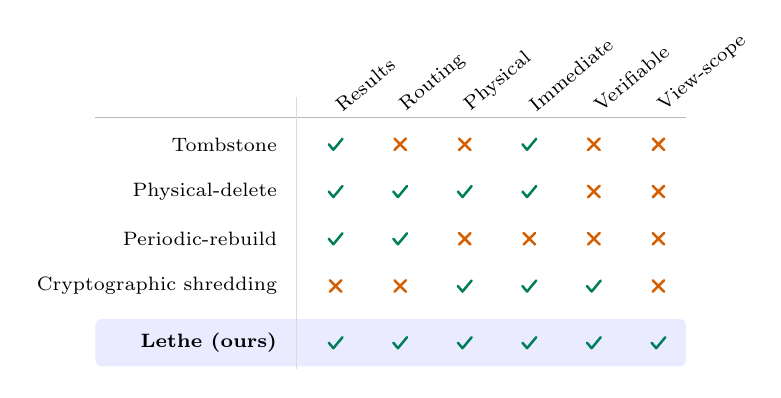
\begin{tikzpicture}[font=\scriptsize]
  % axis column centers
  \def\xa{0}\def\xb{0.82}\def\xc{1.64}\def\xd{2.46}\def\xe{3.28}\def\xf{4.10}
  % row baselines
  \def\rA{0}\def\rB{-0.60}\def\rC{-1.20}\def\rD{-1.80}\def\rL{-2.52}
  % hero shade behind Lethe row (drawn first => sits behind)
  \fill[blue!8,rounded corners=2pt] (-3.05,\rL-0.30) rectangle (4.45,\rL+0.30);
  % rule under header and separator after the label column
  \draw[gray!55] (-3.05,0.34) -- (4.45,0.34);
  \draw[gray!28] (-0.50,0.60) -- (-0.50,\rL-0.34);
  % angled axis headers
  \foreach \x/\t in {\xa/Results,\xb/Routing,\xc/Physical,\xd/Immediate,\xe/Verifiable,\xf/View-scope}{%
    \node[rotate=40,anchor=west,inner sep=1pt] at (\x,0.44) {\t};}
  % row labels
  \node[anchor=east] at (-0.62,\rA) {Tombstone};
  \node[anchor=east] at (-0.62,\rB) {Physical-delete};
  \node[anchor=east] at (-0.62,\rC) {Periodic-rebuild};
  \node[anchor=east] at (-0.62,\rD) {Cryptographic shredding};
  \node[anchor=east] at (-0.62,\rL) {\textbf{\textsc{Lethe} (ours)}};
  % cells: Tombstone
  \node at (\xa,\rA){\cmark};\node at (\xb,\rA){\xmark};\node at (\xc,\rA){\xmark};
  \node at (\xd,\rA){\cmark};\node at (\xe,\rA){\xmark};\node at (\xf,\rA){\xmark};
  % Physical delete
  \node at (\xa,\rB){\cmark};\node at (\xb,\rB){\cmark};\node at (\xc,\rB){\cmark};
  \node at (\xd,\rB){\cmark};\node at (\xe,\rB){\xmark};\node at (\xf,\rB){\xmark};
  % Periodic-rebuild
  \node at (\xa,\rC){\cmark};\node at (\xb,\rC){\cmark};\node at (\xc,\rC){\xmark};
  \node at (\xd,\rC){\xmark};\node at (\xe,\rC){\xmark};\node at (\xf,\rC){\xmark};
  % Cryptographic shred
  \node at (\xa,\rD){\xmark};\node at (\xb,\rD){\xmark};\node at (\xc,\rD){\cmark};
  \node at (\xd,\rD){\cmark};\node at (\xe,\rD){\cmark};\node at (\xf,\rD){\xmark};
  % Lethe
  \node at (\xa,\rL){\cmark};\node at (\xb,\rL){\cmark};\node at (\xc,\rL){\cmark};
  \node at (\xd,\rL){\cmark};\node at (\xe,\rL){\cmark};\node at (\xf,\rL){\cmark};
\end{tikzpicture}%
}
\caption{Erasure capability of index-maintenance methods on the six axes
defined in \S\ref{sec:formal}: whether revoked data is removed from query
\emph{results}, removed from \emph{routing} (traversal), made
\emph{physically} unrecoverable, applied \emph{immediately},
\emph{verifiable}, and scoped to a single \emph{view}. Each prior method
fails at least two axes, and only \textsc{Lethe} achieves per-view erasure.}
\label{fig:matrix}
\end{figure}

We then present \textsc{Lethe}, an index and query-processing design that
satisfies all six axes through four mechanisms, each tied to the axis it
secures. \emph{Revocation-aware traversal} makes ``not routable for the
revoked view'' an invariant of search, so a revoked vector stops steering
that view's queries the moment the revocation is recorded (routing,
immediacy, view scope). An \emph{effective-view-shared bypass overlay}
restores the navigability a revoked vector used to provide, sharing bypass
edges across views so recall holds without an index per user (results,
navigability, memory). Vector-granular \emph{cryptographic
shredding}~\cite{DBLP:journals/corr/abs-2601-07004} supplies the physical,
global erasure the right to be forgotten requires, and an append-only
\emph{erasure log} renders every revocation auditable (physical, verifiable).

We evaluate \textsc{Lethe} on standard ANN benchmarks and access-controlled
clinical, legal, and web corpora, against the most recent streaming-index
and access-controlled baselines. It drives per-view leakage to near zero,
makes globally erased vectors unrecoverable, holds recall close to an oracle
per-view rebuild, sustains high revocation throughput, and uses far less
memory than per-user indexes at billion-vector scale. This paper makes four \textbf{contributions}:
\begin{enumerate}
\item We identify and measure the \emph{zombie vector} phenomenon: in
graph vector indexes, revoked data stays physically recoverable and keeps
routing live queries
(\S\ref{sec:background},~\S\ref{sec:phenomenon}).
\item We formalize \emph{per-view erasure} through six independent axes and
prove no standard primitive achieves it, each violating at least two
(\S\ref{sec:formal}).
\item We design \textsc{Lethe}, the first to satisfy all six axes, with
revocation-aware traversal, an effective-view-shared bypass overlay,
vector-granular cryptographic shredding, and an append-only erasure log
(\S\ref{sec:design},~\S\ref{sec:query}).
\item We evaluate \textsc{Lethe} against recent
streaming-index and access-controlled baselines, with statistical
significance and billion-scale experiments\ifextended; proofs \& full results
are in an extended version (\S\ref{sec:eval}).\else\ (\S\ref{sec:eval}). An extended version, available at \textcolor{blue}{\url{\vldbavailabilityurl}}, provides the full proofs and formal model, the complete baseline comparison and generality study, additional ablations and sensitivity analyses, the security evaluation, and full reproducibility details and statistics.\fi
\end{enumerate}

\section{Background and Threat Model}
\label{sec:background}

\subsection{Graph-based vector indexes}
A graph-based vector index over a dataset $P=\{p_1,\dots,p_N\}$ of $N$ vectors in $d$ dimensions
($P\subset\mathbb{R}^d$) is a directed graph $G=(P,E)$ in which every node is a
vector and each node $p$ stores a short adjacency list of its out-neighbors
$\Nout(p)$, capped at an out-degree bound $M$~\cite{DBLP:journals/pami/MalkovY20,DBLP:conf/nips/SubramanyaDSKK19}.
A query $q$ is answered by greedy best-first traversal: starting from a
fixed entry point, the search keeps a frontier of the $\mathit{ef}$ closest candidates
seen so far ($\mathit{ef}$ trades accuracy for speed), repeatedly expands the closest unexpanded
candidate by visiting its out-neighbors, and stops when the frontier no
longer improves; the $k$ closest visited nodes are
returned~\cite{DBLP:journals/pami/MalkovY20}. We write
$\mathrm{Visit}(q,G)$ for the set of nodes expanded during this traversal,
$R_k(q,G)$ for the $k$ neighbors returned, and measure quality by
$\mathrm{Recall}@k=|R_k(q,G)\cap\mathrm{NN}_k(q)|/k$, the fraction of the
true $k$ nearest neighbors $\mathrm{NN}_k(q)$ recovered. The index works
because $G$ is \emph{navigable}: from the entry point a greedy walk reaches
the neighborhood of $q$ in a few hops, which requires that the nodes along
the way keep pointing toward the rest of the graph.

\begin{figure}[t]
\centering
\definecolor{authc}{RGB}{0,114,178}
\scalebox{\ifextended0.9\else1.0\fi}{%
\begin{tikzpicture}[font=\footnotesize,
   >={Stealth[length=4.5pt]},
   gnode/.style={circle,draw=gray!55,fill=gray!10,minimum size=12pt,inner sep=0pt},
   bnode/.style={circle,draw=leakc,line width=1.6pt,fill=leakc!20,minimum size=14pt,inner sep=0pt},
   rnode/.style={circle,draw=authc,line width=1pt,fill=authc!14,minimum size=14pt,inner sep=0pt},
   enode/.style={circle,draw=black!70,fill=white,minimum size=13pt,inner sep=0pt},
   gedge/.style={draw=gray!45,->},
   pedge/.style={draw=authc,line width=1.3pt,->},
  ]
  \node[enode] (e)  at (0,0.45)   {$e$};
  \node[bnode] (b)  at (1.85,0.15){$b$};
  \node[gnode] (g1) at (1.15,1.5) {};
  \node[gnode] (g2) at (2.95,1.4) {};
  \node[gnode] (g3) at (1.25,-0.95){};
  \node[gnode] (c3) at (3.55,-0.9){};
  \node[rnode] (r1) at (3.75,0.8) {};
  \node[rnode] (r2) at (4.15,-0.15){};
  \node[star,star points=5,star point ratio=2.2,draw=black!70,fill=yellow!85,
        minimum size=11pt,inner sep=0pt] (q) at (4.9,0.1){};
  \begin{scope}[on background layer]
    \draw[gedge] (e)--(g1); \draw[gedge] (b)--(g1); \draw[gedge] (g1)--(g2);
    \draw[gedge] (g2)--(r1); \draw[gedge] (e)--(g3); \draw[gedge] (g3)--(b);
    \draw[gedge] (b)--(c3); \draw[gedge] (c3)--(r2); \draw[gedge] (r1)--(g2);
  \end{scope}
  \draw[pedge] (e)--(b); \draw[pedge] (b)--(r1); \draw[pedge] (r1)--(r2);
  \node[draw=authc,line width=0.8pt,rounded corners=3pt,dashed,
        fit=(r1)(r2),inner sep=4pt] (Rk) {};
  \node[anchor=east,font=\scriptsize] at (e.west) {entry};
  \node[anchor=south,font=\scriptsize,leakc] at ([yshift=1pt]b.north){\,routes, not returned\,};
  \node[anchor=south,font=\scriptsize,authc] at ([xshift=3pt,yshift=2pt]Rk.north){returned $R_k(q,G)$};
  \node[anchor=west,font=\scriptsize] at ([xshift=3pt]q.east) {query $q$};
  \node[anchor=north,font=\scriptsize,authc] at ([yshift=-3pt]e.south east){traversal $\mathrm{Visit}(q,G)$};
\end{tikzpicture}%
}
\caption{Running example. Greedy search for $q$ visits the nodes on the bold
path, $\mathrm{Visit}(q,G)$, but returns only the $k$ nearest, $R_k(q,G)$
(boxed). The bridge $b$ \emph{routes} the query yet is never \emph{returned}.
This separation is what makes revocation subtle: once $b$ is revoked,
Tombstone filters it from $R_k$ but leaves it routing the revoked user's
search (the \emph{zombie} channel of \S\ref{sec:phenomenon}), whereas
\textsc{Lethe} routes around it. We reuse this index throughout the paper.}
\label{fig:example}
\end{figure}

A node $p$ is a \emph{routing waypoint} for $q$ when $p\in\mathrm{Visit}
(q,G)$: the search passes through it, steered onward by its out-edges. This separation between routing and being returned is central to \S\ref{sec:formal}.

\subsection{Deletion and the lazy-repair regime}
Removing a vector $p$ from $G$ is not free. If $p$ is simply dropped, every
in-neighbor $p'\in\Nin(p)$ loses an out-edge, and the walks that used to
pass through $p$ may no longer reach their target, degrading recall.
Restoring navigability requires re-pointing each in-neighbor to suitable
survivors, an operation whose cost grows with
$|\Nin(p)|$~\cite{DBLP:journals/corr/abs-2105-09613}. Because in-degrees
are large in a well-connected index, paying this on every deletion is
prohibitive, so production systems delete \emph{lazily}: a deleted vector
is placed in a tombstone set, excluded from returned results, and its
neighborhood repair is batched into a periodic \emph{consolidation} pass
that runs only after deletions
accumulate~\cite{DBLP:journals/corr/abs-2105-09613}.
Between deletion and consolidation the tombstoned vector remains a node of
$G$ with its edges intact: it is still a routing waypoint, its vector still
occupies memory, and it is written into every serialized snapshot. This
regime is standard and, for freshness, effective.
\S\ref{sec:phenomenon} shows why it becomes unsafe once deletion means
revocation.

\subsection{Multi-tenancy and access control}
A shared index serves a set of principals $U$ (users or roles). An access
policy assigns each vector $p$ an authorized set $A(p)\subseteq U$;
principal $u$'s \emph{view} is the sub-dataset $P_u=\{p\in P: u\in A(p)\}$
it is permitted to retrieve. Permissions are organized as a lattice $L$ of roles with partial order
$\sqsubseteq$, where $\ell'\sqsubseteq\ell$ means role $\ell$ subsumes the
access of role $\ell'$; we then say $\ell$ \emph{dominates} $\ell'$. Each
principal $u$ holds a role $\lambda(u)\in L$ and each vector $p$ is tagged
with the least role $\lambda(p)\in L$ permitted to see it, so $u$ may
retrieve $p$ exactly when $\lambda(p)\sqsubseteq\lambda(u)$; equivalently
$A(p)=\{u\in U:\lambda(p)\sqsubseteq\lambda(u)\}$. For any role $\ell\in L$
we write $P_\ell=\{p\in P:\lambda(p)\sqsubseteq\ell\}$ for the vectors
\emph{visible at} $\ell$; a principal's view is the view of its role,
$P_u=P_{\lambda(u)}$, so principals that share a role share a
view~\cite{DBLP:journals/corr/abs-2505-01538,DBLP:journals/corr/abs-2401-07119}.
Access-controlled vector systems enforce $P_u$ either by partitioning the
index per role or tenant~\cite{DBLP:journals/corr/abs-2505-01538,DBLP:journals/corr/abs-2401-07119}
or by filtering search with a
predicate~\cite{DBLP:journals/pacmmod/PatelKGZ24,DBLP:conf/www/GollapudiKSKBRL23,DBLP:journals/pacmmod/CaiSCZ24},
and relational systems apply row-level security by query
rewriting~\cite{DBLP:conf/sigmod/RizviMSR04}. A \emph{revocation}
$\rev(u,p)$ removes $u$ from $A(p)$, shrinking $P_u$ by one vector while
leaving $P_{u'}$ unchanged for every other principal. \emph{Global erasure},
the right to be forgotten, is the special case that revokes $p$ for all
principals and additionally requires its bytes to be destroyed. The
defining difficulty of revocation, absent from single-tenant deletion, is
that $p$ must vanish from $P_u$ yet stay fully functional in every $P_{u'}$
that still contains it: $p$ cannot be removed from $G$.

\subsection{Threat model and requirements}
We require revocation to take effect against three parties.

\noindent\textbf{(1) Revoked principal.} After $\rev(u,p)$, principal $u$
keeps issuing ordinary queries and observing their results. We treat $u$ as
honest-but-curious: it follows the protocol but may inspect what it
receives. The requirement is that, for every query $u$ issues after
revocation, $p$ neither appears in $u$'s results nor influences which other
vectors do; that is, $u$'s search behaves as if $p$ had never been in
$P_u$. We treat this exposure structurally: because it constrains the index itself rather
than any particular query, this requirement holds for adversarially crafted
queries and under collusion among revoked principals, each of whose view
independently excludes $p$.

\noindent\textbf{(2) Honest-but-curious operator.} For globally erased
vectors, an operator with read access to process memory and to serialized
snapshots must not be able to recover the erased bytes. We assume keys can
be destroyed securely, for example inside a trusted execution
environment~\cite{DBLP:journals/corr/abs-2601-07004}; given that,
cryptographic shredding leaves only ciphertext that cannot be read.

\noindent\textbf{(3) Auditor.} A regulator or compliance auditor is not an
adversary but a stakeholder who must receive verifiable evidence that a
revocation or erasure was requested and took effect, which motivates an
append-only, tamper-evident record.

We assume the index server faithfully enforces the current policy during
traversal, exactly the enforcement we design; compromise of this
reference monitor, timing and other side channels, and inference attacks on
the embedding geometry are out of scope. These parties map directly onto
the axes of Fig.~\ref{fig:matrix}: results, routing, and view scope for the
revoked principal; physical erasure for the operator; verifiability for the
auditor; and immediacy, the requirement that no exploitable window separate
a revocation from its effect, across all three.

\section{The Zombie Vector Phenomenon}
\label{sec:phenomenon}
We now show, by direct measurement on a graph index, that lazy deletion
fails in three concrete ways once it is asked to carry the weight of
revocation. The setup is a clustered HNSW index on which vectors are
revoked by whole semantic cluster, the realistic case in which permissions
follow content (a department, a care unit, a clearance level). All numbers
below are measured; the experimental protocol is in \S\ref{sec:eval}.

\subsection{Revoked vectors are physically retained}
A tombstone is a flag, not an erasure. On a million-scale clustered index, marking a vector deleted leaves the
element count unchanged: the vector keeps its slot. Its embedding is then recoverable in two ways an
operator or auditor would care about. First, the revoked embedding appears
\emph{verbatim} in the serialized index written to disk, so anyone with
read access to the file or a backup obtains it directly. Second, revocation
is reversible: clearing the tombstone returns the embedding byte-for-byte,
even after the index has been saved and reloaded. Logical deletion thus
erases nothing physical: the bytes persist until a consolidation pass
overwrites them.

\subsection{Zombie vectors steer authorized search}
Filtering a vector from the answer does not filter it from the graph. The
bridge $b$ of Fig.~\ref{fig:example} is the single-query picture: once
revoked, $b$ never appears in $R_k$, yet authorized search still routes
through it to reach the vectors beyond. Across a workload this distortion
accumulates as \emph{drift}. To measure it we compare a user's authorized top-10 under Tombstone against an
\emph{oracle} index rebuilt on the authorized vectors alone, the correct
per-view answer; drift is the fraction of that top-10 which differs from the
oracle. Fig.~\ref{fig:dilemma}(a) shows it rising with the revoked fraction,
into the high teens of percent by half the index revoked. The user receives
different answers because of data they are no longer permitted to see.

\begin{figure}[t]
\centering
\includegraphics[width=\columnwidth]{fig_dilemma.pdf}
\caption{The deletion dilemma. \emph{(a)} A revoked vector keeps steering
authorized search: a user's top-10 \emph{drift}, the fraction differing from
an oracle per-view rebuild, grows with the revoked fraction even though
revoked vectors never appear in the results. \emph{(b)} Truly removing a
vector and repairing navigability costs a rebuild that grows with corpus
size; \emph{(c)} bounding the compliance window, how long a revoked vector
may still route, forces a large fraction of machine time into rebuilding, so
cost and retention are inversely coupled. Clustered HNSW on the four datasets
($1.0$--$8.0$M indexed vectors); \emph{(a)} means over ten seeds, bars one standard
deviation; $\mathrm{Recall}@10\,{=}\,0.98$ is the clean oracle index, while
Tombstone falls to about $0.94$ after revocation as routing distortion sets
in; \emph{(b,c)} rebuild cost is the full per-view rebuild; at eight million vectors the graph-build phase alone is $66.8$\,s while the full per-view rebuild reaches $93.0$\,s, means over ten seeds.}
\label{fig:dilemma}
\end{figure}

\subsection{The cost of true erasure, and the compliance window}
There is no cheap way to stop a zombie from routing. The only operation that
removes a revoked vector's influence on traversal is the deferred
consolidation pass, whose limiting case is a full rebuild, work that scales
with the whole corpus rather than the one vector deleted.
Fig.~\ref{fig:dilemma}(b) shows its cost growing to about $93$\,s at eight
million vectors, so paying it on every
revocation is infeasible and systems must batch.
Batching creates a \emph{compliance window}: the longest time a revoked
vector may keep routing before the next pass clears it.
Fig.~\ref{fig:dilemma}(c) makes the trap explicit. Bounding the
window to one minute forces the index to spend most of its time rebuilding,
and at eight million vectors a single rebuild no longer even fits inside the
window; relaxing the window to one hour drops this under $3\%$ but lets
every revoked vector steer queries for that hour. Cost and retention are inversely coupled: under rebuild-based
erasure, one is small only when the other is large.


These are not three problems but one. Tombstone takes a vector out of the
answer but leaves it in the graph, so it still persists and still routes, and
the only operation that removes it rebuilds the whole index.
Erasure under revocation therefore demands what lazy deletion cannot give: a
vector gone from results, from routing, and from storage, immediately, for one
view alone, and verifiably. \S\ref{sec:formal} formalizes this standard;
against it, no existing method stands.

\section{Formalizing Per-View Erasure}
\label{sec:formal}

To rule out those failures we need a precise target: what should it mean to
erase a vector from one principal's view while it stays live for every other?
We answer with six properties, conjoin them into a single guarantee, and prove
no existing maintenance primitive meets it.

\subsection{Erasure requests and the reference view}

We reuse the notation of \S\ref{sec:background}. An index
$\mathcal{I}=(G,S)$ pairs a navigable graph $G=(P,E)$ over the stored
vectors $P$ with a physical store $S$ holding their bytes. A query for
principal $u$ returns $\mathrm{Ans}(\mathcal{I},q,u)$, the returned
top-$k$ over $u$'s view (the principal-aware form of $R_k$ from
\S\ref{sec:background}), and its greedy traversal expands a set of
nodes $\mathrm{Visit}(\mathcal{I},q,u)\subseteq P$ (the principal-aware form of
$\mathrm{Visit}(q,G)$, now ranging over the full index $\mathcal{I}$ and
principal $u$). The view of $u$ is
$P_u=\{p\in P: u\in A(p)\}$.

An \emph{erasure request} $\rho=(p,R)$ names a vector $p$ and a scope
$R\subseteq U$ of principals who must lose access to it. Revoking a single
principal is $R=\{u\}$; global erasure is $R=U$. After $\rho$ is
applied, $u\notin A(p)$ for every $u\in R$, so $p\notin P_u$.

To say what $u$ \emph{should} observe once $p$ leaves its view, we fix a
reference: $\mathcal{I}^\star_u$, the index built on exactly $P_u$. This is
the oracle per-view rebuild of \S\ref{sec:phenomenon}: the behavior an index
would have if $p$, and every other vector $u$ cannot see, had never been
inserted for $u$.

\subsection{The six axes}

\begin{table}[t]
\centering
\small
\setlength{\tabcolsep}{5pt}
\renewcommand{\arraystretch}{1.2}
\caption{The six axes of per-view erasure (Definition~\ref{def:pve}): each
names a way a revoked vector $p$ can persist after a request $\rho=(p,R)$
transforms the index $\mathcal{I}$ into $\mathcal{I}'$ with store $S'$. $\mathrm{Ans}$ and $\mathrm{Visit}$ are the answer and visited sets of
\S\ref{sec:background}; $R{=}U$ is global erasure.}
\label{tab:axes}
\scalebox{0.8}{%
\begin{tabularx}{\columnwidth}{@{}l X@{}}
\toprule
Axis & Condition on $\mathcal{I}'$ \\
\midrule
\textsc{Results}    & $p\notin\mathrm{Ans}(\mathcal{I}',q,u)$ for every $u\in R$ and query $q$ \\
\textsc{Routing}    & $p\notin\mathrm{Visit}(\mathcal{I}',q,u)$: $p$ is never distance-scored, inserted into the frontier, expanded, or returned\,$^{a}$ \\
\textsc{Physical}   & if $R{=}U$, $p$'s bytes are unrecoverable from $S'$, in memory and every serialized snapshot \\
\textsc{Immediate}  & the conditions above hold from the moment $\rho$ is accepted \\
\textsc{Verifiable} & a tamper-evident record lets a third party confirm $\rho$ took effect \\
\textsc{View-scope} & every $u'\notin R$ with $p\in P_{u'}$ keeps access to $p$ and its recall\,$^{b}$ \\
\bottomrule
\end{tabularx}%
}

\vspace{2pt}
{\footnotesize $^{a}$\,$p$'s identifier may still be \emph{encountered} in an
adjacency list the search scans, since $p$ stays a physical node shared with
views that still hold it; the axis forbids $p$'s \emph{participation}, not its
appearance in an edge list.\quad
$^{b}$\,Not bit-for-bit identical: \S\ref{sec:eval} measures the small
top-$k$ drift on unaffected views.}
\end{table}

A mechanism that answers $\rho=(p,R)$ by transforming $\mathcal{I}$ into
$\mathcal{I}'$ may satisfy the six properties of Table~\ref{tab:axes}.
Routing is strictly stronger than Results: a method may hide $p$ from the
answer yet still let it bend the path that selects the other returned
vectors, the zombie effect measured in \S\ref{sec:phenomenon}. We
keep the two separate because existing methods achieve one without the
other.

\begin{definition}[Per-view erasure]
\label{def:pve}
A mechanism achieves \emph{per-view erasure} if, for every request
$\rho=(p,R)$, the resulting index satisfies \textsc{Results},
\textsc{Routing}, \textsc{Immediate}, \textsc{Verifiable}, and
\textsc{View-scope} for the scope $R$, and additionally \textsc{Physical}
whenever $R=U$.
\end{definition}

The reference $\mathcal{I}^\star_u$ is an empirical quality target, not
part of the definition: per-view erasure pins down $p$'s operational
non-participation exactly, while \S\ref{sec:eval} shows the resulting
answers track $\mathcal{I}^\star_u$ to within its own seed-to-seed
variation, rather than claiming identity with it.

We call the quantity Definition~\ref{def:pve} drives to zero the
\emph{per-view leakage} of $p$ into a revoked view: any way in which $p$
still reaches $u$ after revocation, whether through a returned result or
through a traversal it steers. This is a structural property of the index,
separate from inference about hidden data, which we do not study.

\subsection{No existing primitive suffices}

\begin{theorem}
\label{thm:sixaxis}
Each of Tombstone, Physical-delete, Periodic-rebuild, and
cryptographic shredding violates at least two of the six axes. Hence none
of them, applied alone, achieves per-view erasure.
\end{theorem}

\begin{proof}
For each primitive we exhibit an axis it cannot satisfy;
Fig.~\ref{fig:matrix} records the full pattern.

\emph{Tombstone} flags $p$ deleted and filters it from answers
(\textsc{Results}) instantly (\textsc{Immediate}), but leaves $p$ a node of
$G$ with its edges intact. It therefore keeps steering traversal
(\textsc{Routing} fails; \S\ref{sec:phenomenon} measures the drift)
and keeps its bytes in memory and snapshots (\textsc{Physical} fails). A
mutable flag carries no proof of erasure (\textsc{Verifiable} fails), and
it removes $p$ for all principals at once rather than for a chosen view
(\textsc{View-scope} fails).

\emph{Physical-delete} removes $p$'s node and repairs its in-neighbors,
so $p$ neither appears in nor routes any answer (\textsc{Results},
\textsc{Routing}) and its bytes are gone from the live store
(\textsc{Physical}). But it acts on every principal (\textsc{View-scope}
fails) and produces no auditable record (\textsc{Verifiable} fails).

\emph{Periodic-rebuild} reconstructs the graph on the surviving
set, satisfying \textsc{Results} and \textsc{Routing} once it runs. But it
runs only at the next scheduled pass: until then $p$ survives in the live
store, so its bytes stay recoverable and the compliance window of
\S\ref{sec:phenomenon} stays open on the physical axis as well
(\textsc{Physical} and \textsc{Immediate} fail). It is also global
(\textsc{View-scope} fails) and unaudited (\textsc{Verifiable} fails).

\begin{sloppypar}
\emph{Cryptographic shredding} destroys $p$'s key, rendering its bytes
unreadable (\textsc{Physical}) at once (\textsc{Immediate}) and checkably
so (\textsc{Verifiable}). But it changes the bytes, not the graph: $p$'s
node and edges remain and no predicate excludes them, so the search still
scores, expands, and can return $p$ (\textsc{Routing}, \textsc{Results}
fail); the bytes are merely unreadable, so the distance $p$ contributes is
meaningless rather than absent. And a key is bound to a record, not to a
view (\textsc{View-scope} fails).
\end{sloppypar}

The \textsc{View-scope} column is thus empty for every prior primitive, and
no single primitive covers \textsc{Routing}, \textsc{Physical},
\textsc{Immediate}, and \textsc{View-scope} together.
\end{proof}

The proof points to what a solution must combine: view-scoped control of
both results and traversal, global byte destruction when the scope is
everyone, and a single operation that is immediate and leaves an auditable
trace. \S\ref{sec:design} builds exactly this.\ifextended\ Appendix~\ref{app:formal} gives the full
formal model and the complete proofs.\fi

\section{\textsc{Lethe}: Design}
\label{sec:design}

\S\ref{sec:formal} fixed the target. Per-view erasure reads like a
demand for a separate index per view; \textsc{Lethe} meets it over \emph{one} shared
structure, augmenting a standard navigable graph (HNSW or DiskANN) with four
cooperating elements, each closing one or more axes of
Definition~\ref{def:pve}.

\subsection{Overview}

\textsc{Lethe} keeps the base graph $G=(P,E)$ intact and adds four elements:

\begin{enumerate}
\item a per-vector \emph{access predicate} consulted during search, which
  makes ``$p$ is transparent for view $u$'' an invariant of traversal
  (\textsc{Results}, \textsc{Routing}, \textsc{Immediate},
  \textsc{View-scope});
\item an \emph{effective-view-shared bypass overlay} that restores the
  navigability a revoked vector used to provide, without materializing a
  separate graph per user (preserving recall, hence \textsc{View-scope} for
  authorized principals);
\item \emph{vector-granular cryptographic shredding} that destroys a
  vector's bytes once its scope reaches everyone (\textsc{Physical});
\item an \emph{append-only erasure log} that records every revocation and
  shred in tamper-evident form (\textsc{Verifiable}).
\end{enumerate}

A revocation never rebuilds or repairs the graph eagerly, so it takes effect
on the very next query. Figure~\ref{fig:arch} traces how a query and an
erasure request move through these elements over the one shared index.

\begin{figure}[t]
\centering
\resizebox{\columnwidth}{!}{%
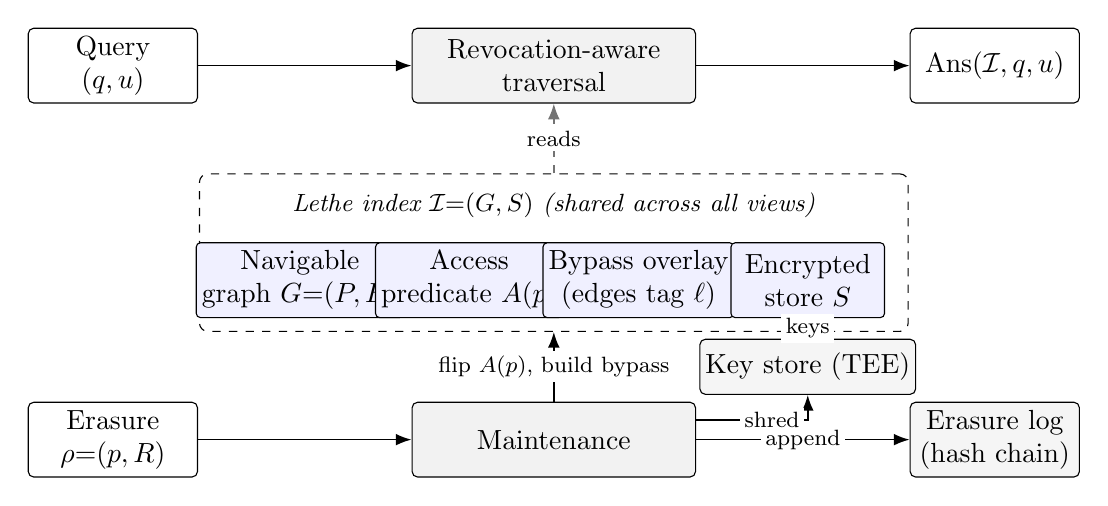
\begin{tikzpicture}[
  font=\normalsize,
  io/.style={draw, rounded corners=2pt, align=center, minimum width=2.15cm, minimum height=0.95cm, inner sep=2pt},
  proc/.style={draw, rounded corners=2pt, align=center, minimum width=3.6cm, minimum height=0.95cm, inner sep=2pt, fill=black!5},
  store/.style={draw, rounded corners=2pt, align=center, minimum width=2.15cm, minimum height=0.95cm, inner sep=2pt, fill=black!4},
  ann/.style={draw, rounded corners=2pt, align=center, minimum width=2.05cm, minimum height=0.7cm, inner sep=2pt, fill=black!4},
  cell/.style={draw, rounded corners=1.5pt, align=center, minimum width=1.95cm, minimum height=0.95cm, inner sep=2pt, fill=blue!6},
  lbl/.style={font=\footnotesize, fill=white, inner sep=1.6pt},
  fl/.style={-{Latex[length=2mm]}, semithick},
  rd/.style={-{Latex[length=2mm]}, semithick, draw=black!55, dashed},
]
\node[draw, dashed, rounded corners=3pt, minimum width=9cm, minimum height=2.0cm] (idx) at (7,2.775) {};
\node[font=\small\itshape, anchor=north] at ([yshift=-1.2mm]idx.north) {Lethe index $\mathcal{I}{=}(G,S)$ (shared across all views)};
\node[cell] (g)  at (3.775,2.425) {Navigable\\graph $G{=}(P,E)$};
\node[cell] (ap) at (5.925,2.425) {Access\\predicate $A(p)$};
\node[cell] (bo) at (8.075,2.425) {Bypass overlay\\(edges tag $\ell$)};
\node[cell] (s)  at (10.225,2.425) {Encrypted\\store $S$};
\node[io]    (q)    at (1.40,5.15) {Query\\$(q,u)$};
\node[proc]  (trav) at (7.00,5.15) {Revocation-aware\\traversal};
\node[io]    (ans)  at (12.60,5.15) {$\mathrm{Ans}(\mathcal{I},q,u)$};
\node[io]    (er)   at (1.40,0.40) {Erasure\\$\rho{=}(p,R)$};
\node[proc]  (maint) at (7.00,0.40) {Maintenance};
\node[store] (log)  at (12.60,0.40) {Erasure log\\(hash chain)};
\node[ann]   (ks)   at (10.225,1.325) {Key store (TEE)};
\draw[fl] (q.east)      -- (trav.west);
\draw[fl] (trav.east)   -- (ans.west);
\draw[fl] (er.east)     -- (maint.west);
\draw[fl] (maint.east)  -- (log.west)  node[lbl,pos=0.5]{append};
\draw[rd] (idx.north)   -- (trav.south) node[lbl,midway]{reads};
\draw[fl] (maint.north) -- (idx.south)  node[lbl,midway]{flip $A(p)$, build bypass};
\draw[fl] ([yshift=2.5mm]maint.east) -| (ks.south) node[lbl,pos=0.34]{shred};
\draw[fl] (ks.north)    -- (s.south)   node[lbl,midway]{keys};
\end{tikzpicture}%
}
\caption{\textsc{Lethe} over one shared index, with the query path (top) and the
erasure path (bottom) mirrored. A query $(q,u)$ is answered by
revocation-aware traversal, which reads the graph $G$, the access predicate
$A(p)$, and the bypass overlay. An erasure request $\rho=(p,R)$ drives
maintenance that flips $A(p)$ and builds bypass edges
(Alg.~\ref{alg:bypass}), appends to the erasure log, and shreds the
vector's key in the key store, which holds the per-vector keys that decrypt
the encrypted store $S$; destroying a key renders that vector's bytes
unreadable. Dashed edges are reads, solid edges are writes.}
\label{fig:arch}
\end{figure}


\subsection{Revocation-aware traversal}

\textsc{Lethe} attaches to each vector $p$ its access set $A(p)$, stored compactly
as a bitmap over the roles of the permission lattice $L$
(\S\ref{sec:background}), together with a small per-principal exception
set recording individual grants or revocations layered on the role grant, so
a revocation can target a whole role or a single principal; the test
$u\in A(p)$ is $O(1)$. Greedy
search proceeds as usual with one change at every expanded node $p$: if
$u\notin A(p)$, then $p$ is \emph{transparent} to $u$. A transparent node is
never entered into the result candidate set and never ranked, so it can
neither appear in nor reorder $u$'s answer (\textsc{Results}); and its
distance never enters the frontier that selects the next node to expand, so
it exerts no routing influence (\textsc{Routing}). Reachability past $p$ is
preserved by the overlay below, not by following $p$'s own edges. Because
the test reads live metadata, removing $u$ from $A(p)$ takes effect on the
next query with no structural change (\textsc{Immediate}) and alters nothing
for any $u'$ that still holds $p$ (\textsc{View-scope}).

\subsection{The effective-view-shared bypass overlay}

Making $p$ transparent removes a connector: $p$ may have been the only short
link between two regions of $u$'s authorized subgraph, and dropping it is
exactly the navigability-corrupting ghost of \S\ref{sec:phenomenon}.
Repairing this separately for each principal would rebuild a graph per user,
the memory blow-up \textsc{Lethe} must avoid.

The repair, however, depends not on the individual principal but on the
\emph{effective view}: the view $P_u$ of \S\ref{sec:background}, the vectors $u$ may actually see once
role grants and any individual exceptions are applied. Principals with the
same effective view need the same bypass around $p$. Under pure role-based
access these classes coincide with the lattice elements, and the bypass is
computed once per role; an individual revocation that splits a role refines
it into separate effective-view classes, leaving a still-authorized principal
of that role undisturbed. \textsc{Lethe} therefore keys the bypass by effective-view
class, written $\ell$ below, not by user.

Alg.~\ref{alg:bypass} builds it. Let $\mathrm{Prune}(x,\mathit{cand},M)$
denote the base index's own neighbor-selection heuristic, which returns at
most $M$ close yet diverse neighbors of $x$ from a candidate set
$\mathit{cand}$ (\textsc{RobustPrune} in
DiskANN~\cite{DBLP:conf/nips/SubramanyaDSKK19}, the analogous heuristic in
HNSW~\cite{DBLP:journals/pami/MalkovY20}), with $M$ the out-degree bound of
\S\ref{sec:background}. When $p$ becomes transparent across an effective-view class
$\ell$, the survivors it used to reach are its authorized out-neighbors
$C=\Nout(p)\cap P_\ell$. For each authorized in-neighbor
$a\in\Nin(p)\cap P_\ell$, which previously routed through $p$ to reach $C$,
\textsc{Lethe} re-selects $a$'s neighbors over its current ones together with $C$
using $\mathrm{Prune}$, and records the newly chosen edges in the overlay,
tagged $\ell$. This is the same local repair a physical deletion would
apply, but confined to $P_\ell$ and written to the overlay rather than into
$G$.

\begin{algorithm}
\caption{Bypass construction for a transparent vector}
\label{alg:bypass}
\begin{algorithmic}[1]
\Require vector $p$, transparent across effective-view class $\ell$; base graph $G$;
out-degree bound $M$; pruning heuristic $\mathrm{Prune}$
\Ensure overlay edges, tagged $\ell$, restoring navigability of $P_\ell$ around $p$
\State $C \gets \Nout(p)\cap P_\ell$ \Comment{authorized survivors reached via $p$}
\For{each $a \in \Nin(p)\cap P_\ell$} \Comment{authorized in-neighbors routed via $p$}
  \State $T \gets \mathrm{Prune}\big(a,\ (\Nout(a)\cup C)\cap P_\ell,\ M\big)$
  \For{each $b \in T\setminus \Nout(a)$}
    \State add overlay edge $a\!\rightarrow\! b$ tagged $\ell$
  \EndFor
\EndFor
\end{algorithmic}
\end{algorithm}

\begin{sloppypar}
Each construction touches only $p$'s neighborhood: it prunes
$|\Nin(p)\cap P_\ell|$ in-neighbors over $O(M)$ candidates each, for
$O(|\Nin(p)|\cdot M)$ distance computations and no global rebuild. It runs
once per $(p,\ell)$ and is reused by every principal in effective-view
class $\ell$ that lost $p$. When $p$ is transparent to $u$, the query follows the base edges
of $G$ together with the bypass edges tagged with $u$'s effective-view
class, whose endpoints lie in $P_u$ and are therefore all visible to $u$. The construction does not recreate the edges a rebuild on $P_\ell$ would
produce, overlapping them only partly (\S\ref{sec:eval}); it restores
navigability instead, so greedy search reaches the authorized neighborhood
nearly as well as on a rebuild, up to the pruning approximation. The overlay's size scales with the number of
distinct $(p,\ell)$ repairs, bounded by the number of effective-view classes:
the lattice elements under pure role-based access, refining only where
individual exceptions split a role. \S\ref{sec:eval} shows it stays far
below a per-user index, rising from $1.24\times$ to $1.29\times$ the base
graph as the exception rate grows from zero to one half, while holding recall
close to $\mathcal{I}^\star_u$.
\end{sloppypar}

\subsection{Vector-granular cryptographic shredding}

Transparency hides $p$ but does not destroy it. That is correct for
revocation, where others still need $p$, but insufficient when the scope is
everyone. \textsc{Lethe} stores each vector's payload encrypted under a per-vector
key, with keys kept outside the index in a protected key store such as a
trusted execution environment, following
MemTrust~\cite{DBLP:journals/corr/abs-2601-07004}. Erasing $p$ for all
principals destroys its key: the ciphertext that remains in memory and in
every snapshot can no longer be read (\textsc{Physical}); the destruction is
instantaneous (\textsc{Immediate}); and destroying a named key is itself the
evidence an auditor checks. The unreadable node is then made transparent to
every view through the same predicate, with bypass edges installed at the
top of the lattice, so global erasure reuses the traversal and overlay for
results and routing and adds only byte destruction.

\subsection{The append-only erasure log}

Verifiability must not rest on the operator's word. \textsc{Lethe} records every
request $\rho=(p,R)$ as an entry in an append-only, hash-chained log: the
scope, a timestamp, and a commitment to the affected vector, signed so that
entries cannot be altered or reordered without detection. An auditor checks
two facts without trusting the operator: that the log is intact as an
append-only chain, and that the live index agrees with it, namely that
$p$'s predicate excludes exactly $R$ and, for a global erasure, that $p$'s
key is gone. Each erasure thus becomes a checkable fact
(\textsc{Verifiable}).

\subsection{Composition}

A revocation alters only $p$'s neighborhood, at constant or amortized cost
and without a rebuild; \S\ref{sec:query} gives the procedure and its
complexity. The four mechanisms compose to the full guarantee:

\begin{proposition}
\label{prop:lethe}
\textsc{Lethe} achieves per-view erasure (Definition~\ref{def:pve}):
revocation-aware traversal secures \textsc{Results}, \textsc{Routing},
\textsc{Immediate}, and the traversal half of \textsc{View-scope}; the
effective-view-shared bypass overlay secures the recall half of
\textsc{View-scope}; the append-only erasure log secures \textsc{Verifiable};
and vector-granular cryptographic shredding secures \textsc{Physical} when
$R=U$.
\end{proposition}

\noindent The per-mechanism arguments are the four subsections above; the
navigability of the bypass overlay, that it preserves authorized recall while
removing the revoked node from every revoked view's reachable set, is proved
in the extended version. \textsc{Lethe} thus fills the row left empty in
Fig.~\ref{fig:matrix}, over one structure shared across views.

\section{Query Processing and Maintenance}
\label{sec:query}

\S\ref{sec:design} fixed the mechanisms; this section gives the search
and maintenance procedures over them, with their costs.

\subsection{Revocation-aware search}

Alg.~\ref{alg:search} answers a query $q$ for principal $u$. It is the
greedy best-first search of \S\ref{sec:background} with two changes,
both keyed to $u$'s effective-view class $\mathrm{ev}(u)$, its role $\lambda(u)$ when no individual exception applies. First, a visited node $b$ enters the
frontier and the answer only when $u\in A(b)$; a transparent node
($u\notin A(b)$) is skipped, so it is neither ranked nor returned
(\textsc{Results}) and its distance never steers the search
(\textsc{Routing}). Second, when expanding a node $a$ the search follows
$a$'s base out-edges together with $a$'s bypass edges tagged $\mathrm{ev}(u)$,
written $\mathrm{Bypass}_{\mathrm{ev}(u)}(a)$; these detour around the
transparent nodes $a$ used to reach (\S\ref{sec:design}). We write
$\mathit{ef}$ for the frontier width and take the entry point $\mathit{ep}$ to be a
navigation node, visible to every role and never a revocation target.

\begin{algorithm}
\caption{Revocation-aware search}
\label{alg:search}
\begin{algorithmic}[1]
\Require query $q$; principal $u$; entry point $\mathit{ep}$; frontier width $\mathit{ef}$; result size $k$
\Ensure the $k$ vectors of $P_u$ nearest to $q$
\State $W \gets \{\mathit{ep}\}$ \Comment{frontier of authorized candidates}
\While{$W$ has an unexpanded node}
  \State $a \gets$ unexpanded node of $W$ nearest to $q$; mark $a$ expanded
  \For{each $b \in \Nout(a)\cup \mathrm{Bypass}_{\mathrm{ev}(u)}(a)$}
    \If{$b$ not yet visited}
      \State mark $b$ visited
      \If{$u\in A(b)$} \Comment{transparent nodes are skipped}
        \State $W \gets W \cup \{b\}$; keep the $\mathit{ef}$ nodes of $W$ nearest to $q$
      \EndIf
    \EndIf
  \EndFor
\EndWhile
\State \Return the $k$ nodes of $W$ nearest to $q$
\end{algorithmic}
\end{algorithm}

The access test $u\in A(b)$ is $O(1)$ (\S\ref{sec:ds}). The traversal
otherwise visits the region a base search over $P_u$ would, because
$\mathrm{Bypass}_{\mathrm{ev}(u)}$ restores the reachability a rebuild on
$P_u$ would have (\S\ref{sec:design}) and its out-degree is bounded
like the base graph's by $M$. Search therefore keeps
the base greedy-search cost, $O(\mathit{ef}\cdot M\cdot d)$ distance work
along the walk for $d$-dimensional vectors, plus an $O(1)$ test per visited
node. Recall matches the oracle per-view rebuild up to the pruning approximation of
\S\ref{sec:design}, which \S\ref{sec:eval} measures.

\subsection{Maintenance}

Alg.~\ref{alg:maint} applies an erasure request $\rho=(p,R)$. It
removes $R$ from $A(p)$, a constant-time predicate update; for each effective-view
class $\ell$ whose view $P_\ell$ loses $p$ it ensures the bypass edges of
Alg.~\ref{alg:bypass} exist, building them once and sharing them across
that class's principals; for a global request ($R=U$) it destroys $p$'s key;
and it appends one entry to the erasure log. No step rebuilds the graph.

\begin{algorithm}
\caption{Maintenance for an erasure request}
\label{alg:maint}
\begin{algorithmic}[1]
\Require request $\rho=(p,R)$; key store; append-only erasure log
\State $A(p) \gets A(p)\setminus R$ \Comment{$O(1)$ predicate update}
\For{each effective-view class $\ell\in\mathcal{L}(R)$} \Comment{classes whose view $P_\ell$ loses $p$}
  \If{the bypass around $p$ tagged $\ell$ is not yet built}
    \State run Alg.~\ref{alg:bypass} on $(p,\ell)$
  \EndIf
\EndFor
\If{$R = U$}
  \State destroy $p$'s key in the key store \Comment{cryptographic shredding}
\EndIf
\State append $\langle p,\,R,\,\text{timestamp},\,\mathrm{commit}(p)\rangle$ to the erasure log
\end{algorithmic}
\end{algorithm}

Let $\mathcal{L}(R)$ be the set of effective-view classes whose view loses $p$
under $\rho$: one class for a single-role revocation, $\mathrm{ev}(u)$ for a
single-principal revocation $R=\{u\}$, and every class whose view contained $p$ for a global request $R=U$. The
predicate update is $O(1)$; each bypass build is $O(|\Nin(p)|\cdot M)$
(Alg.~\ref{alg:bypass}) and runs once per $(p,\ell)$; key destruction
and the signed, hash-chained log append are $O(1)$. Maintenance therefore
costs $O(|\mathcal{L}(R)|\cdot|\Nin(p)|\cdot M)$, local to $p$'s
neighborhood, against the $\Theta(N)$ of a consolidation pass over $N$
vectors. It takes effect on the next query.

Concurrency and crash recovery turn on one rule: a revocation linearizes at
the predicate commit. Once $A(p)\setminus R$ is published, every query
is denied $p$ on Results and Routing, while the bypass build and log append
may lag, as they bear on recall and audit, not reachability. After a
crash, recovery restores the committed predicate and, for $R=U$, confirms the
key is destroyed, so a revoked vector never reappears; \S\ref{sec:eval}
reports zero leakage after recovery, against the residue from methods recovering to a stale graph\ifextended; Appendix~\ref{app:crash} drives a crash at each point of the maintenance and recovery path and confirms a zero-leakage safe state from every one\fi.

\subsection{Data structures and space}
\label{sec:ds}

Each vector $p$ carries its role tag $\lambda(p)$ and a short exception list
of principals revoked from the role-induced default; the test $u\in A(p)$
then checks $\lambda(p)\sqsubseteq\lambda(u)$ against a precomputed
reachability bitmap over the lattice and scans the exception list, in
$O(1)$. The bypass overlay is stored as, for each node $a$, its bypass
edges grouped by tag $\ell$, so that $\mathrm{Bypass}_{\mathrm{ev}(u)}(a)$ is a
single lookup. Its total size is $\sum_{(p,\ell)}|\Nin(p)\cap P_\ell|\cdot M$
over the built repairs, bounded by the number of (vector, class) repairs
rather than by the user population, and far below the
$\Theta(|L|\cdot N\cdot M)$ of materializing one graph per role. Building those edges needs $p$'s
in-neighbors $\Nin(p)$, which a graph storing only out-edges does not
provide; \textsc{Lethe} keeps a reverse-edge directory, updated on insertion, that
returns $\Nin(p)$ in a few milliseconds by lookup, an order of magnitude
under the full-graph scan the alternative would require, with a high
in-degree hub the worst case (\S\ref{sec:eval}). The erasure
log is an append-only hash chain holding one signed record per request,
$O(|\text{requests}|)$ in size. The base graph $G$ and the encrypted store
$S$ are untouched by revocation, so a deployment pays only for the predicate
bits, the reverse-edge directory, the overlay it actually uses, and the log.

\section{Evaluation}
\label{sec:eval}

Our evaluation establishes four claims, in the order a skeptical reader
would test them. First, the routing channel is real: a revoked vector that
has been filtered from every result still steers the queries of the very
view it was revoked from, and the effect is large enough to measure and to
exploit. Second, result filtering is therefore not erasure, because the
channel it leaves open is the one a graph index depends on to navigate.
Third, \textsc{Lethe} closes both the routing channel and the physical
residue while holding recall at the level of an oracle per-view rebuild and
leaving unaffected views untouched. Fourth, it does so at a cost that is
acceptable against the three alternatives a practitioner would otherwise
reach for: rebuilding the index, materializing one index per view, and
filtering search. We take these in turn after fixing the setup.

\subsection{Setup}
\label{sec:eval-setup}

\paragraph{Datasets.}
We use four corpora chosen to separate a graph-index property from a
text-encoder artifact. Three are access-controlled text collections: a
legal corpus built on LegalBench~\cite{DBLP:conf/nips/GuhaNHRCKCPWRZT23} in
a retrieval-augmented configuration~\cite{DBLP:conf/icail/BarronESMA25}, an
open-domain web collection from MS~MARCO~\cite{DBLP:conf/sigir/CraswellMYCL21}
under a synthesized role hierarchy, and
MIMIC-IV~\cite{PhysioNet-mimiciv-3.1,DBLP:journals/scientificdata/JohnsonBSGSHPHMGLCM23}
clinical notes as a sensitive-domain case
study~\cite{DBLP:journals/jhir/SivarajkumarMORHLHVW24}. The fourth,
SIFT1M~\cite{DBLP:journals/pami/JegouDS11}, carries exact ground truth and
no text encoder, so the zombie effect appearing there shows it is a property
of graph navigation rather than of any embedding model. Text corpora are
embedded once with BGE-large-en-v1.5~\cite{DBLP:conf/sigir/XiaoLZMLN24} at 1024
dimensions and cached, so every method reads identical vectors.

\paragraph{Permission workload.}
On top of each corpus we generate \textsc{SharedConfidential}, an
overlapping role-based access structure in which each vector belongs to one
or more roles, 80\% of vectors are shared across several roles and 20\% are
role-private, and role popularity follows a Zipfian distribution. Users are
assigned to roles, and a revocation withdraws a subset of the shared vectors
from one user or role while every other principal that holds them stays
authorized. We sweep the revoked fraction from 0 to 0.5 and the revocation
pattern over random, hub, and cluster. Cluster is the primary pattern: permissions in practice track semantic
groups, a document class or a care unit, so a revocation removes a coherent
region of the embedding space rather than scattered points, the regime in
which a graph index is hardest to keep navigable and that most stresses any
erasure mechanism.\ifextended\ Sensitivity to the predicate exception rate, to user-level revocation within a shared role, and to view distance from the revoked principal is reported in Appendices~\ref{app:exception}, \ref{app:samerole}, and~\ref{app:viewscope}.\else\ Sensitivity to the predicate exception rate, to user-level revocation within a shared role, and to view distance from the revoked principal is reported in the extended version.\fi

\paragraph{Index and operating point.}
\begin{sloppypar}
All methods index the same vectors with
HNSW~\cite{DBLP:journals/pami/MalkovY20} through hnswlib at top-$k$ with
$k{=}10$, out-degree $M{=}16$, and \texttt{ef\_construction}${=}200$. We
fix a single \texttt{ef\_search} across all methods and revoked fractions,
tuned so the oracle per-view rebuild reaches Recall@10 $\approx 0.98$ on the
authorized set; the methods therefore share one search budget, and the
differences in Recall@10 reported in Section~\ref{sec:eval-recall} come from
how each method indexes and filters rather than from a different operating
point. The
characterization runs use single-threaded, fully seeded builds, which make
the graph, and therefore the drift it produces, reproducible across
machines; throughput, scalability, and concurrency runs use multiple threads
and are reported as trends. Exact ground truth is computed by blocked
$\ell_2$ search. Generality to a second graph index,
DiskANN~\cite{DBLP:conf/nips/SubramanyaDSKK19}, and to a second encoder is
reported in \ifextended Appendix~\ref{app:diskann} (Table~\ref{tab:diskann})\else the extended version\fi.
\end{sloppypar}

\paragraph{Baselines.}
We compare against the alternatives a practitioner can deploy today, all
on the same vectors, search budget, and workload. \emph{Tombstone}
marks a revoked vector deleted and filters it from results while leaving it
in the graph, the production default~\cite{DBLP:journals/corr/abs-2105-09613}.
\emph{Post-filter} enforces access by row-level security over a shared
index~\cite{DBLP:conf/sigmod/RizviMSR04}. \emph{Physical-delete} removes the
vector and repairs only the affected neighborhoods, and
\emph{Periodic-rebuild} consolidates the whole index on a
schedule~\cite{DBLP:journals/corr/abs-2105-09613}. \emph{Per-role-index}
materializes a separate index per role, the cost upper bound a per-view
guarantee naively
implies~\cite{DBLP:journals/corr/abs-2505-01538,DBLP:journals/corr/abs-2401-07119}.
\emph{ACORN}~\cite{DBLP:journals/pacmmod/PatelKGZ24} and
\emph{HoneyBee}~\cite{DBLP:journals/corr/abs-2505-01538} are
predicate-filtered and role-partitioned access-controlled indexes, and
\emph{SPFresh}~\cite{DBLP:conf/sosp/XuLLXCZLYYYCY23} is a streaming in-place
maintenance system. \emph{Oracle} rebuilds an index on exactly the
authorized vectors of each view; it is the gold standard for what an erased
index should return, and we use it as the reference for drift and recall
rather than as a deployable baseline.

\paragraph{Metrics.}
Every top-10 list below is restricted to authorized vectors, so a revoked
vector can never appear in a result and any divergence we report comes from
routing rather than from a leaked answer. \emph{Result leakage} is the
fraction of a returned top-10 that are revoked vectors, and it is zero by
construction for every method that filters results. \emph{Top-10 drift} is one
minus the average overlap between a method's authorized top-10 and the
top-10 of the \emph{Oracle} per-view rebuild, taken over the query workload;
it measures how far routing through revoked vectors bends the answer away
from a truly erased index. \emph{Operational leakage} instruments the
search loop and reports the fraction of traversal events, namely distance
evaluations, frontier insertions, and expansions, that
touch a revoked vector; it is the routing component of \emph{per-view
leakage} (\S\ref{sec:formal}) and measures the zombie mechanism directly,
so drift cannot be dismissed as approximation noise. \emph{Recall@10} is the overlap
of the authorized top-10 with the exact ten nearest authorized neighbors. To
ground leakage in an adversary's success we add two attacks: a
\emph{distinguishing} test reports the AUC of the strongest classifier that
decides, from observed outputs, whether a revoked vector still influences a
view, where 0.5 means indistinguishable from the \emph{Oracle}; and a
\emph{reconstruction} attack runs embedding inversion~\cite{DBLP:conf/emnlp/MorrisKSR23} on bytes recovered from
a serialized snapshot and reports token F1 and exact match. Cost is measured
by revocation throughput, the compliance window (\S\ref{sec:phenomenon}), memory relative to per-user
and per-role materialization, and a per-query latency breakdown.

\paragraph{Protocol.}
The headline results, the existence of the channel, operational leakage, recall,
and view isolation, use ten seeds; ablation, memory, and compliance-window
results use five. We report the mean and standard deviation over seeds, the
bootstrap 95\% confidence interval of the gap to \textsc{Lethe} ($10^5$
resamples, stratified by dataset and revocation pattern), a paired bootstrap
significance test with Holm-Bonferroni correction across the baselines in
each table, and a rank-biserial effect size. We use a bootstrap rather than
a signed-rank test because, when one method dominates another on every
paired run, a rank test is bounded by its own discrete resolution rather
than by the evidence. Seeds, tests, and corrections are fixed before
running. Machine-dependent quantities, latency, throughput, and scaling, are
reported as trends with the machine stated and carry no significance tests,
since their absolute values are not comparable across hardware.\ifextended\ Appendix~\ref{app:repro} gives the full datasets, build configuration, and artifact manifest.\fi

\subsection{A revoked vector still routes}
\label{sec:eval-exists}

\begin{figure}[t]
\centering
\includegraphics[width=\columnwidth]{fig_zombie.pdf}
\caption{A revoked vector is gone from the answer and still steering the
search. Result leakage is zero for every method, so a revoked vector never
appears in a result and all divergence shown here is routing.
\emph{(a)} The fraction of traversal events that distance-score, insert into
the frontier, or expand a revoked vector reaches 25.9\% under Tombstone and
29.2\% under Post-filter at half the index revoked, because both keep
revoked vectors in the graph; \textsc{Lethe} encounters a revoked identifier
but never scores, inserts, or expands it, so the value is identically zero and
coincides with the oracle per-view rebuild. \emph{(b)} The authorized top-10
consequently drifts from a truly erased index, by 17.6\% (Tombstone) and
18.9\% (Post-filter) at the same point, against 0.9\% for \textsc{Lethe}.
\emph{(c)} A classifier given only a user's own outputs separates a
tombstoned or post-filtered index from the oracle at AUC up to 0.88 and
0.86, while \textsc{Lethe} stays at 0.51, on the random line.
\textsc{SharedConfidential}, cluster revocation, four datasets, ten seeds;
bars are one standard deviation.}
\label{fig:zombie}
\end{figure}

Filtering a revoked vector out of the result is easy, and every method does
it: result leakage is zero throughout (Fig.~\ref{fig:zombie}). The quantity
that matters is what the search does on the way to that result.
Figure~\ref{fig:zombie}(a) measures it by instrumenting the traversal. Under
Tombstone, the production default, the fraction of traversal events that
touch a revoked vector climbs with the revoked fraction, reaching 25.9\% at
one half; Post-filter is marginally worse, and a lazily
repairing streaming index, SPFresh, still routes through revoked vectors at
the same point. The cause is structural. All
three leave the revoked vectors in the graph, so the walk keeps visiting
them, expanding them, and scoring their neighbors on every query, for the
very user from whom they were revoked.

This traversal changes the answer. Figure~\ref{fig:zombie}(b) shows the
authorized top-10 drifting from the result an index would return had the
vectors truly been removed, by 17.6\% under Tombstone at half the index
revoked. Because revoked vectors are
filtered from the result, every one of these differences is a reordering
among \emph{authorized} vectors. The revoked vectors are not appearing in
the answer, they are deciding which permitted vectors do. The effect is
largest under cluster revocation, where a withdrawn semantic region leaves a
gap the walk must cross, the access pattern that arises whenever
permissions track a document class or a care unit.


Whether a curious user can act on this is Fig.~\ref{fig:zombie}(c). A
classifier given nothing but a user's own top-10 outputs separates a
tombstoned index from an oracle per-view rebuild at an AUC of 0.88 at half
revocation, with the advantage growing
monotonically in how much has been revoked. The residual routing influence
is therefore not only measurable by us under full instrumentation but
recoverable by an adversary holding nothing but black-box access to its own
results. The signal is the continued presence of the revoked vectors; an
index that had erased them would offer nothing to separate.

The ordering holds on every dataset: Figure~\ref{fig:perdataset} breaks it
down per collection, with \textsc{Lethe} holding drift to 0.7--1.2\% across
collections, matching the per-role index at a fraction of its memory, while Tombstone and Post-filter sit at 17--19\%.

% Per-dataset drift heatmap. Requires \usetikzlibrary is not needed.
% Source: leakage_recall.csv (cluster, frac=0.5, mean over four datasets x ten seeds).
\begin{figure}[t]
\centering
\definecolor{leakc}{RGB}{213,94,0}%
\definecolor{lethe}{RGB}{0,114,178}%
\resizebox{\ifextended0.725\else0.9\fi\columnwidth}{!}{%
\begin{tikzpicture}[x=1cm,y=1cm]
\fill[leakc!0!white] (0.000,0.000) rectangle (1.180,-0.460);
\node[font=\scriptsize, black] at (0.590,-0.230) {0.0};
\fill[leakc!0!white] (1.180,0.000) rectangle (2.360,-0.460);
\node[font=\scriptsize, black] at (1.770,-0.230) {0.0};
\fill[leakc!0!white] (2.360,0.000) rectangle (3.540,-0.460);
\node[font=\scriptsize, black] at (2.950,-0.230) {0.0};
\fill[leakc!0!white] (3.540,0.000) rectangle (4.720,-0.460);
\node[font=\scriptsize, black] at (4.130,-0.230) {0.0};
\fill[leakc!5!white] (0.000,-0.460) rectangle (1.180,-0.920);
\node[font=\scriptsize, black] at (0.590,-0.690) {1.1};
\fill[leakc!3!white] (1.180,-0.460) rectangle (2.360,-0.920);
\node[font=\scriptsize, black] at (1.770,-0.690) {0.7};
\fill[leakc!6!white] (2.360,-0.460) rectangle (3.540,-0.920);
\node[font=\scriptsize, black] at (2.950,-0.690) {1.2};
\fill[leakc!4!white] (3.540,-0.460) rectangle (4.720,-0.920);
\node[font=\scriptsize, black] at (4.130,-0.690) {0.8};
\fill[leakc!2!white] (0.000,-0.920) rectangle (1.180,-1.380);
\node[font=\scriptsize, black] at (0.590,-1.150) {0.4};
\fill[leakc!3!white] (1.180,-0.920) rectangle (2.360,-1.380);
\node[font=\scriptsize, black] at (1.770,-1.150) {0.6};
\fill[leakc!3!white] (2.360,-0.920) rectangle (3.540,-1.380);
\node[font=\scriptsize, black] at (2.950,-1.150) {0.7};
\fill[leakc!3!white] (3.540,-0.920) rectangle (4.720,-1.380);
\node[font=\scriptsize, black] at (4.130,-1.150) {0.6};
\fill[leakc!20!white] (0.000,-1.380) rectangle (1.180,-1.840);
\node[font=\scriptsize, black] at (0.590,-1.610) {4.2};
\fill[leakc!20!white] (1.180,-1.380) rectangle (2.360,-1.840);
\node[font=\scriptsize, black] at (1.770,-1.610) {4.3};
\fill[leakc!20!white] (2.360,-1.380) rectangle (3.540,-1.840);
\node[font=\scriptsize, black] at (2.950,-1.610) {4.1};
\fill[leakc!20!white] (3.540,-1.380) rectangle (4.720,-1.840);
\node[font=\scriptsize, black] at (4.130,-1.610) {4.3};
\fill[leakc!29!white] (0.000,-1.840) rectangle (1.180,-2.300);
\node[font=\scriptsize, black] at (0.590,-2.070) {6.1};
\fill[leakc!29!white] (1.180,-1.840) rectangle (2.360,-2.300);
\node[font=\scriptsize, black] at (1.770,-2.070) {6.1};
\fill[leakc!30!white] (2.360,-1.840) rectangle (3.540,-2.300);
\node[font=\scriptsize, black] at (2.950,-2.070) {6.2};
\fill[leakc!30!white] (3.540,-1.840) rectangle (4.720,-2.300);
\node[font=\scriptsize, black] at (4.130,-2.070) {6.2};
\fill[leakc!35!white] (0.000,-2.300) rectangle (1.180,-2.760);
\node[font=\scriptsize, black] at (0.590,-2.530) {7.3};
\fill[leakc!35!white] (1.180,-2.300) rectangle (2.360,-2.760);
\node[font=\scriptsize, black] at (1.770,-2.530) {7.3};
\fill[leakc!36!white] (2.360,-2.300) rectangle (3.540,-2.760);
\node[font=\scriptsize, black] at (2.950,-2.530) {7.5};
\fill[leakc!35!white] (3.540,-2.300) rectangle (4.720,-2.760);
\node[font=\scriptsize, black] at (4.130,-2.530) {7.3};
\fill[leakc!40!white] (0.000,-2.760) rectangle (1.180,-3.220);
\node[font=\scriptsize, black] at (0.590,-2.990) {8.5};
\fill[leakc!40!white] (1.180,-2.760) rectangle (2.360,-3.220);
\node[font=\scriptsize, black] at (1.770,-2.990) {8.3};
\fill[leakc!40!white] (2.360,-2.760) rectangle (3.540,-3.220);
\node[font=\scriptsize, black] at (2.950,-2.990) {8.5};
\fill[leakc!40!white] (3.540,-2.760) rectangle (4.720,-3.220);
\node[font=\scriptsize, black] at (4.130,-2.990) {8.4};
\fill[leakc!51!white] (0.000,-3.220) rectangle (1.180,-3.680);
\node[font=\scriptsize, black] at (0.590,-3.450) {10.8};
\fill[leakc!52!white] (1.180,-3.220) rectangle (2.360,-3.680);
\node[font=\scriptsize, white] at (1.770,-3.450) {11.0};
\fill[leakc!53!white] (2.360,-3.220) rectangle (3.540,-3.680);
\node[font=\scriptsize, white] at (2.950,-3.450) {11.1};
\fill[leakc!52!white] (3.540,-3.220) rectangle (4.720,-3.680);
\node[font=\scriptsize, black] at (4.130,-3.450) {10.9};
\fill[leakc!84!white] (0.000,-3.680) rectangle (1.180,-4.140);
\node[font=\scriptsize, white] at (0.590,-3.910) {17.6};
\fill[leakc!83!white] (1.180,-3.680) rectangle (2.360,-4.140);
\node[font=\scriptsize, white] at (1.770,-3.910) {17.5};
\fill[leakc!84!white] (2.360,-3.680) rectangle (3.540,-4.140);
\node[font=\scriptsize, white] at (2.950,-3.910) {17.6};
\fill[leakc!84!white] (3.540,-3.680) rectangle (4.720,-4.140);
\node[font=\scriptsize, white] at (4.130,-3.910) {17.7};
\fill[leakc!90!white] (0.000,-4.140) rectangle (1.180,-4.600);
\node[font=\scriptsize, white] at (0.590,-4.370) {19.0};
\fill[leakc!90!white] (1.180,-4.140) rectangle (2.360,-4.600);
\node[font=\scriptsize, white] at (1.770,-4.370) {18.9};
\fill[leakc!90!white] (2.360,-4.140) rectangle (3.540,-4.600);
\node[font=\scriptsize, white] at (2.950,-4.370) {18.9};
\fill[leakc!90!white] (3.540,-4.140) rectangle (4.720,-4.600);
\node[font=\scriptsize, white] at (4.130,-4.370) {18.8};
\draw[white,line width=0.6pt] (0,0) grid[xstep=1.18,ystep=0.46] (4.720,-4.600);
\draw[gray!55,line width=0.5pt] (0,0) rectangle (4.720,-4.600);
\node[font=\scriptsize\itshape, gray!50!black, anchor=east] at (-0.12,-0.230) {Oracle};
\node[font=\scriptsize\bfseries, lethe, anchor=east] at (-0.12,-0.690) {Lethe};
\node[font=\scriptsize, anchor=east] at (-0.12,-1.150) {Per-role-index};
\node[font=\scriptsize, anchor=east] at (-0.12,-1.610) {Physical-delete};
\node[font=\scriptsize, anchor=east] at (-0.12,-2.070) {HoneyBee};
\node[font=\scriptsize, anchor=east] at (-0.12,-2.530) {ACORN};
\node[font=\scriptsize, anchor=east] at (-0.12,-2.990) {Periodic-rebuild};
\node[font=\scriptsize, anchor=east] at (-0.12,-3.450) {SPFresh};
\node[font=\scriptsize, anchor=east] at (-0.12,-3.910) {Tombstone};
\node[font=\scriptsize, anchor=east] at (-0.12,-4.370) {Post-filter};
\node[font=\scriptsize, align=center, anchor=south] at (0.590,0.08) {Legal-\\Bench};
\node[font=\scriptsize, align=center, anchor=south] at (1.770,0.08) {MIMIC-\\IV};
\node[font=\scriptsize, align=center, anchor=south] at (2.950,0.08) {MS-\\MARCO};
\node[font=\scriptsize, align=center, anchor=south] at (4.130,0.08) {SIFT\\1M};
\fill[leakc!100!white] (5.060,-4.600) rectangle (5.360,-4.485);
\fill[leakc!97!white] (5.060,-4.485) rectangle (5.360,-4.370);
\fill[leakc!95!white] (5.060,-4.370) rectangle (5.360,-4.255);
\fill[leakc!92!white] (5.060,-4.255) rectangle (5.360,-4.140);
\fill[leakc!90!white] (5.060,-4.140) rectangle (5.360,-4.025);
\fill[leakc!87!white] (5.060,-4.025) rectangle (5.360,-3.910);
\fill[leakc!85!white] (5.060,-3.910) rectangle (5.360,-3.795);
\fill[leakc!82!white] (5.060,-3.795) rectangle (5.360,-3.680);
\fill[leakc!79!white] (5.060,-3.680) rectangle (5.360,-3.565);
\fill[leakc!77!white] (5.060,-3.565) rectangle (5.360,-3.450);
\fill[leakc!74!white] (5.060,-3.450) rectangle (5.360,-3.335);
\fill[leakc!72!white] (5.060,-3.335) rectangle (5.360,-3.220);
\fill[leakc!69!white] (5.060,-3.220) rectangle (5.360,-3.105);
\fill[leakc!67!white] (5.060,-3.105) rectangle (5.360,-2.990);
\fill[leakc!64!white] (5.060,-2.990) rectangle (5.360,-2.875);
\fill[leakc!62!white] (5.060,-2.875) rectangle (5.360,-2.760);
\fill[leakc!59!white] (5.060,-2.760) rectangle (5.360,-2.645);
\fill[leakc!56!white] (5.060,-2.645) rectangle (5.360,-2.530);
\fill[leakc!54!white] (5.060,-2.530) rectangle (5.360,-2.415);
\fill[leakc!51!white] (5.060,-2.415) rectangle (5.360,-2.300);
\fill[leakc!49!white] (5.060,-2.300) rectangle (5.360,-2.185);
\fill[leakc!46!white] (5.060,-2.185) rectangle (5.360,-2.070);
\fill[leakc!44!white] (5.060,-2.070) rectangle (5.360,-1.955);
\fill[leakc!41!white] (5.060,-1.955) rectangle (5.360,-1.840);
\fill[leakc!38!white] (5.060,-1.840) rectangle (5.360,-1.725);
\fill[leakc!36!white] (5.060,-1.725) rectangle (5.360,-1.610);
\fill[leakc!33!white] (5.060,-1.610) rectangle (5.360,-1.495);
\fill[leakc!31!white] (5.060,-1.495) rectangle (5.360,-1.380);
\fill[leakc!28!white] (5.060,-1.380) rectangle (5.360,-1.265);
\fill[leakc!26!white] (5.060,-1.265) rectangle (5.360,-1.150);
\fill[leakc!23!white] (5.060,-1.150) rectangle (5.360,-1.035);
\fill[leakc!21!white] (5.060,-1.035) rectangle (5.360,-0.920);
\fill[leakc!18!white] (5.060,-0.920) rectangle (5.360,-0.805);
\fill[leakc!15!white] (5.060,-0.805) rectangle (5.360,-0.690);
\fill[leakc!13!white] (5.060,-0.690) rectangle (5.360,-0.575);
\fill[leakc!10!white] (5.060,-0.575) rectangle (5.360,-0.460);
\fill[leakc!8!white] (5.060,-0.460) rectangle (5.360,-0.345);
\fill[leakc!5!white] (5.060,-0.345) rectangle (5.360,-0.230);
\fill[leakc!3!white] (5.060,-0.230) rectangle (5.360,-0.115);
\fill[leakc!0!white] (5.060,-0.115) rectangle (5.360,0.000);
\draw[gray!55,line width=0.4pt] (5.060,-4.600) rectangle (5.360,0.000);
\node[font=\tiny, anchor=west] at (5.390,-4.600) {20};
\node[font=\tiny, anchor=west] at (5.390,-2.410) {10};
\node[font=\tiny, anchor=west] at (5.390,-0.219) {0};
\node[font=\scriptsize, rotate=90, anchor=south] at (6.140,-2.300) {Top-10 drift (\%)};
\end{tikzpicture}%
}
\caption{The zombie effect and \textsc{Lethe}'s correction are consistent across datasets. Top-10 drift of the authorized answer from a per-view rebuild (\%), per method and per dataset, at half the index revoked. The ordering and magnitudes are stable across all four collections: the oracle is exact, \textsc{Lethe} holds drift to 0.7--1.2\% (matching the per-role index without its memory cost), while Tombstone and Post-filter drift by 17--19\% on every dataset. \textsc{SharedConfidential}, cluster revocation, mean over ten seeds.}
\label{fig:perdataset}
\end{figure}

The vector persists in more than the traversal. The other half of the zombie
definition is physical: can the revoked content be recovered from what the
system still stores?\ifextended\ Appendix~\ref{app:security} reports the inference attacks, adversarial revocation targeting, and audit tamper-evidence behind this.\fi\ Table~\ref{tab:phys-recovery} pairs byte-exact recovery from a
serialized snapshot with the embedding-inversion reconstruction run on
whatever bytes that recovery yields. Every method that leaves the vector's bytes on disk, including the access-control overlays of ACORN and HoneyBee,
keeps it byte-exact in the snapshot and reconstructable at token
F1 0.42 with half the index revoked; only the methods that remove the bytes, \textsc{Lethe}'s cryptographic shredding among them, drop
reconstruction to 0.01, the floor for a vector that was never stored. Tombstone misses the physical axis as squarely as it
misses routing: the revoked embedding sits one snapshot read and one inversion
away.

\begin{table}[t]
\centering
\small
\setlength{\tabcolsep}{6pt}
\caption{Physical persistence of a globally erased vector: whether its bytes survive
byte-exact in a serialized snapshot (\emph{Byte-rec.}), and the token F1 of an
embedding-inversion reconstruction from the recovered bytes (\emph{Recon.\ F1}).
\textsc{SharedConfidential}, four datasets; the reconstruction runs only on
the three with a text encoder, mean over ten seeds with half the index
revoked. The 0.01 floor is the
reconstruction of a vector the system never stored.}
\label{tab:phys-recovery}
\begin{tabular*}{\columnwidth}{@{\extracolsep{\fill}}lcrlcr@{}}
\toprule
Method & Byte- & Recon. & Method & Byte- & Recon. \\
       & rec.  & F1     &        & rec.  & F1     \\
\midrule
Tombstone   & \cmark & 0.42 & Periodic-rebuild & \cmark & 0.42 \\
Post-filter & \cmark & 0.42 & Physical-delete  & \xmark & 0.01 \\
SPFresh     & \cmark & 0.41 & Per-role-index   & \xmark & 0.01 \\
ACORN       & \cmark & 0.42 & \cellcolor{letherow}\textsc{Lethe}   & \cellcolor{letherow}\xmark & \cellcolor{letherow}0.01 \\
HoneyBee    & \cmark & 0.42 & Oracle           & \xmark & 0.01 \\
\bottomrule
\end{tabular*}
\end{table}

\textsc{Lethe} behaves throughout like the oracle, not the production
default. Its operational leakage is identically zero, because
revocation-aware traversal makes a revoked vector unreachable for the view, not merely absent from the result; its drift is 0.9\% at half
revocation, an order of magnitude below Tombstone; and its distinguishing
AUC is 0.51, on the random line. The gap between \textsc{Lethe} and
methods that keep the vector is consistent across all four datasets and
every seed: at half revocation \textsc{Lethe} is better on every paired run,
so the rank-biserial effect size is $-1.0$ on leakage and drift and $+1.0$
on recall, the 95\% bootstrap confidence interval of each gap excludes zero,
and a paired bootstrap test is significant at $p\le 0.001$ on every
dataset after Holm correction.\ifextended\ The full per-cell statistics for all
$48$ comparisons appear in Appendix~\ref{app:stats}.\fi\ The result is the one filtering cannot reach: a
revoked vector is gone from the answer under every method, yet still steers
the search; and once globally erased, its bytes stay recoverable on disk under every method keeping the shared graph navigable, \textsc{Lethe} alone excepted.

\subsection{Erasure without losing recall or disturbing other views}
\label{sec:eval-recall}

\begin{figure}[t]
\centering
\includegraphics[width=\columnwidth]{fig_recall.pdf}
\caption{\textsc{Lethe} reaches the answer quality of an oracle per-view
rebuild without its cost, and changes only the view requesting the
revocation. \emph{(a)} Recall@10 against revoked fraction. \textsc{Lethe}
holds 0.976, just under half a point below the oracle and more than three points
above Physical-delete (0.944) and Tombstone (0.940), which repair only
locally or not at all and lose navigability. \emph{(b)} Each method placed by the revoked user's drift from
the answer it should now receive ($x$) and an unaffected user's drift from the
answer it should still receive ($y$), both against a per-view rebuild; the
origin is ideal. Tombstone and Post-filter spare unaffected users but
fail the revoked one (21.0\% and 9.3\%, the zombie effect); Physical-delete
erases but restructures the shared index and so disturbs still-authorized users, raising the view-isolation violation rate to 39.0\%. Only
\textsc{Lethe} and the per-role index reach the corner. \textsc{SharedConfidential}, cluster revocation, four datasets; panel
(b) at 80\% shared vectors, high role overlap, and 100 roles, and error bars
are one standard deviation.}
\label{fig:recall}
\end{figure}

A per-view guarantee is worthless if it degrades the answer it protects, and there are two ways it could. The authorized user could lose
recall, or the residual drift we just measured could be uncaught leakage
rather than benign approximation error. Figure~\ref{fig:recall}(a) settles
the first. \textsc{Lethe} holds Recall@10 at 0.976 across the
revocation range, a hair below the oracle per-view rebuild and well clear
of Physical-delete's recall cost ($p\le 0.001$, paired bootstrap).
Physical-delete is the cautionary case: removing the vector and repairing
only its local neighborhood damages navigability and costs recall, exactly the
expense the bypass overlay is designed to avoid.

The second concern is ruled out by decomposing the drift against the oracle
into the part any approximate index incurs and the part that is genuine
erasure residue. The approximation floor is fixed independently of
\textsc{Lethe}: two independently seeded oracle rebuilds of the same
authorized set drift 0.45\% from each other. \textsc{Lethe}'s 0.9\% sits just
above this floor, the gap being the bypass overlay's pruning approximation
rather than erasure residue, so its answer is, to measurement, a per-view
rebuild. Tombstone and Post-filter instead drift 17.6\% and 18.9\%,
leaving 17.1 and 18.5 points that the floor cannot explain. That residue is
the zombie routing of \S\ref{sec:eval-exists},
now read as error in the delivered result rather than as traffic in the
traversal.

Erasure must also stay local to the view that asked for it: revoking a
vector from one user must not move what another user who still holds it
retrieves. Figure~\ref{fig:recall}(b) plots each method's two drifts
against its own correct per-view rebuild, and they divide along exactly the
axis the formal model predicts. Tombstone and Post-filter spare the
unaffected user but abandon the revoked one; Physical-delete inverts this:
it erases, but because it mutates the single shared index it disturbs users
who still have access, pushing the view-isolation violation rate to 39.0\%.
Only \textsc{Lethe} and the per-role index hold both ends, keeping the
unaffected user more than an order of magnitude tighter than Physical-delete ($p\le 0.001$).

The leakage is not only geometric; it reaches the answer the user reads.
Feeding each method's retrieved set to a fixed open 7B generator on
LegalBench-RAG (Table~\ref{tab:rag}) shows that routing through revoked
vectors costs end-to-end quality: Tombstone and Post-filter lose more
than three F1 points against an oracle per-view rebuild, while \textsc{Lethe}
matches the oracle, 55.5 against 55.8. The zombie vectors do not merely change
which authorized neighbors are retrieved; they degrade the answer generated
from them.

\begin{table}[t]
\centering
\small
\setlength{\tabcolsep}{6pt}
\caption{End-to-end retrieval-augmented generation quality on LegalBench-RAG
with a fixed open 7B generator (\%). Methods that do not alter the returned
set are omitted.}
\label{tab:rag}
\begin{tabular*}{\columnwidth}{@{\extracolsep{\fill}}lrrlrr@{}}
\toprule
Method & Exact match & F1 & Method & Exact match & F1 \\
\midrule
Post-filter & 38.90 & 52.36 & HoneyBee       & 41.31 & 54.34 \\
Tombstone   & 39.40 & 52.76 & \cellcolor{letherow}\textsc{Lethe} & \cellcolor{letherow}42.80 & \cellcolor{letherow}55.48 \\
ACORN       & 40.90 & 53.84 & Oracle         & 43.20 & 55.80 \\
\bottomrule
\end{tabular*}
\end{table}

\textsc{Lethe} thus reaches a corner the other deployable methods cannot
hold at once: the recall and erasure quality of an oracle rebuild together
with the view isolation of an index that was never restructured. The per-role
index reaches the same corner and the oracle defines it; what does each pay to
get there?

\subsection{The cost of getting there}
\label{sec:eval-cost}

\begin{table}[t]
\centering
\small
\caption{Cost of erasure. Revocations per second and the compliance window,
the longest time a revoked vector keeps routing, are throughput measurements
on one machine and are reported as trends. Memory is index size relative to
the base graph. Filtering methods are cheap but never erase, so their window
spans the consolidation interval; methods that do erase pay in throughput
(Physical-delete, Periodic-rebuild) or in memory (the per-role index).
\textsc{Lethe} pays neither. \textsc{SharedConfidential}, four
datasets, mean over five seeds.}
\label{tab:cost}
\setlength{\tabcolsep}{4pt}
\begin{tabular}{lrrr}
\toprule
       & Revocations & Compliance & Memory \\
Method & per second  & window (s) & ($\times$base) \\
\midrule
Tombstone        &  95{,}077 & 3800.0 &   1.00 \\
SPFresh          &  17{,}011 &   0.05 &   1.08 \\
Physical-delete  &   2{,}461 &    0.05 &  0.96 \\
Periodic-rebuild &  10{,}931 &  651.6 &   1.06 \\
Per-role-index   &   4{,}000 &    0.05 &  84.25 \\
\rowcolor{letherow}\textsc{Lethe}   &  49{,}975 &  0.004 &   1.26 \\
\bottomrule
\end{tabular}
\end{table}

\begin{figure}[t]
\centering
\definecolor{lethe}{RGB}{0,114,178}%
\definecolor{leakc}{RGB}{213,94,0}%
\definecolor{costc}{RGB}{120,120,128}%
\definecolor{good}{RGB}{0,158,115}%
\scalebox{\ifextended0.76\else0.8\fi}{%
\begin{tikzpicture}
\definecolor{pfilt}{RGB}{230,159,0}%
\begin{axis}[
  width=\columnwidth, height=0.635\columnwidth,
  xmode=log, log basis x=10,
  xmin=1700, xmax=300000, ymin=-3.4, ymax=33,
  xlabel={Revocation throughput (revocations/s)},
  ylabel={Operational leakage (\%)},
  xlabel style={font=\footnotesize}, ylabel style={font=\footnotesize},
  tick label style={font=\footnotesize},
  axis line style={gray!55},
  xtick={10000,100000}, xticklabels={$10^4$,$10^5$},
  extra x ticks={2000,5000,20000,50000,200000}, extra x tick labels={},
  extra x tick style={grid=none, tick style={gray!40}},
  ytick={0,10,20,30},
  ymajorgrids, grid style={gray!18, very thin},
  clip=false,
]
\fill[good!13] (axis cs:35000,-3.4) rectangle (axis cs:300000,3.2);
\draw[good!45!black, dashed, very thin] (axis cs:35000,3.2) -- (axis cs:300000,3.2);
\node[good!50!black, font=\footnotesize\itshape, anchor=south east, align=right]
   at (axis cs:285000,-3.1) {no leakage,\\high throughput};
\draw[->, >=Latex, good!55!black, thin] (axis cs:17000,4.2) -- (axis cs:38200,1.0);
\node[good!55!black, font=\footnotesize\itshape, anchor=east] at (axis cs:17400,4.7) {better};
\node[circle,fill=pfilt,draw=pfilt!55!black,inner sep=2pt] at (axis cs:92000,29.2){};
\node[circle,fill=leakc,draw=leakc!55!black,inner sep=2pt] at (axis cs:95077,25.9){};
\node[circle,fill=leakc,draw=leakc!55!black,inner sep=2pt] at (axis cs:17011,14.5){};
\node[circle,fill=leakc,draw=leakc!55!black,inner sep=2pt] at (axis cs:24000,8.3){};
\node[circle,fill=leakc,draw=leakc!55!black,inner sep=2pt] at (axis cs:26000,7.0){};
\node[circle,fill=leakc,draw=leakc!55!black,inner sep=2pt] at (axis cs:10931,9.4){};
\node[font=\scriptsize, anchor=east] at (axis cs:81000,29.2) {Post-filter};
\node[font=\scriptsize, anchor=east] at (axis cs:86000,25.9) {Tombstone};
\node[font=\scriptsize, anchor=west] at (axis cs:19200,14.5) {SPFresh};
\node[font=\scriptsize, anchor=south] at (axis cs:24000,9.2) {ACORN};
\node[font=\scriptsize, anchor=west] at (axis cs:29000,7.0) {HoneyBee};
\node[font=\scriptsize, anchor=east] at (axis cs:9900,9.4) {Periodic-rebuild};
\node[circle,fill=costc,draw=costc!60!black,inner sep=2pt] at (axis cs:2461,0){};
\node[circle,fill=costc!85,draw=costc!60!black,inner sep=7pt] at (axis cs:4000,0){};
\node[font=\scriptsize, anchor=south west] at (axis cs:1820,1.9) {Physical-delete};
\node[font=\scriptsize, anchor=west, align=left, costc!30!black]
   at (axis cs:8000,0.1) {Per-role-index\\\textbf{84$\times$ memory}};
\node[star, star points=5, star point ratio=2.2, fill=lethe, draw=lethe!45!black,
      line width=0.5pt, inner sep=3.2pt] at (axis cs:49975,0){};
\node[lethe!72!black, font=\small\bfseries, anchor=south] at (axis cs:49975,2.9) {Lethe};
\end{axis}
\end{tikzpicture}%
}
\caption{Throughput, leakage, and memory across erasure methods. Each method is
placed by revocation throughput ($x$, log scale) and operational leakage at
half revocation ($y$); marker size reflects index memory, with the per-role
index drawn conspicuously large. Methods that retain the revoked vector are cheap but leak (upper region);
methods that erase it pay in throughput (left) or in memory (the per-role index,
$84\times$ the base graph at 100 roles); only \textsc{Lethe} reaches the corner of no leakage
at high throughput and near-base memory. The oracle per-view rebuild carries no
steady-state revocation cost and is omitted. \textsc{SharedConfidential}, cluster
revocation, four datasets; throughput and memory over five seeds, operational leakage as in \S\ref{sec:eval-exists} over ten
seeds.}
\label{fig:dominance}
\end{figure}

Table~\ref{tab:cost} and Fig.~\ref{fig:dominance} show it:
every baseline is pushed out of the corner along the axis it pays on.\ifextended\ Appendix~\ref{app:baseline} gives the complete thirteen-method comparison across all six axes.\fi The cheapest-looking methods
never erase. Tombstone sustains 95{,}000 revocations per second,
but its compliance window is 3{,}800 seconds, because nothing removes the
vector from the graph until a full consolidation runs; its throughput is that of doing nothing. The methods that do erase pay for it, along
opposite axes: Physical-delete holds the window near zero at the cost of
throughput, while Periodic-rebuild buys throughput back only by leaving a
window where the vector still routes. This is the compliance-window trap of
\S\ref{sec:phenomenon} made concrete: with erasure bound to a structural
pass, a short window costs throughput and high throughput costs a long
window.

The per-role index escapes the trap by giving each role its own index, so a
revocation is immediate, but it pays in memory: one materialized index per
role costs 84 times the base graph at 100 roles and grows linearly in the
number of roles, reaching 421 times at 500 roles. \textsc{Lethe} obtains the same per-view erasure for
$1.26\times$ the base graph, flat in the number of roles while the per-role
index grows linearly, $1.5\%$ of the per-role index at 100
roles ($0.3\%$ at 500) and $0.0014\%$ of a per-user index, a materialization
that at 100{,}000 users would cost $88{,}000\times$ the base graph, because the bypass
edges are shared across principals with the same effective view instead of
being replicated per role or per user.

\textsc{Lethe} alone pays none of these. It erases immediately, with a
0.004-second window that is five to six orders of magnitude below the
consolidation- and rebuild-based methods; it sustains 50{,}000 revocations
per second, the highest of any method that actually erases; and it does so at
base-index memory. The query path absorbs the predicate check and overlay
lookup at a 95th-percentile latency of 16.0\,ms, fourteen percent over
Tombstone and below every method that restructures the graph.
\textsc{Lethe}'s five added query-path components total 1.1\,ms over the base
graph search, within twelve percent of Tombstone; the extended version
decomposes the mean per-query latency per component. The design
holds at scale. At one billion vectors a query returns in 7.8\,ms and a
revocation applies in 0.057\,ms, the overlay adding 193\,GB to a 3.0\,TB
index; the same near-oracle drift and zero operational leakage hold on
DiskANN/Vamana and a second encoder
\ifextended (Table~\ref{tab:diskann})\else (extended version)\fi. The compliance-window
trap is not a law of nature but a consequence of binding erasure to the index
structure; move erasure into the traversal and the structure never has to be
rebuilt, so immediacy costs neither throughput nor~memory.

\subsection{Each mechanism secures one axis}
\label{sec:eval-ablation}

\begin{table}[t]
\centering
\caption{Ablation of \textsc{Lethe}. Removing a mechanism forfeits the one
axis of Fig.~\ref{fig:matrix} it secures and leaves the others intact:
revocation-aware traversal secures routing, the bypass overlay secures
navigability (recall), cryptographic shredding secures physical
unrecoverability, and the erasure log secures verifiability. The last two
rows isolate the design choice behind the memory result of
\S\ref{sec:eval-cost}; \emph{per-user overlay} replaces the effective-view-shared
overlay with one materialized per user. \textsc{SharedConfidential}, cluster revocation, four
datasets, mean over five seeds. Column headers abbreviate operational leakage (\emph{Oper.\ leak.}), physically unrecoverable (\emph{Phys.\ unrec.}), and memory (\emph{Mem.}); \emph{Recall@10} and \emph{Auditable} are line-wrapped, not abbreviated.}
\label{tab:ablation}
\resizebox{\columnwidth}{!}{%
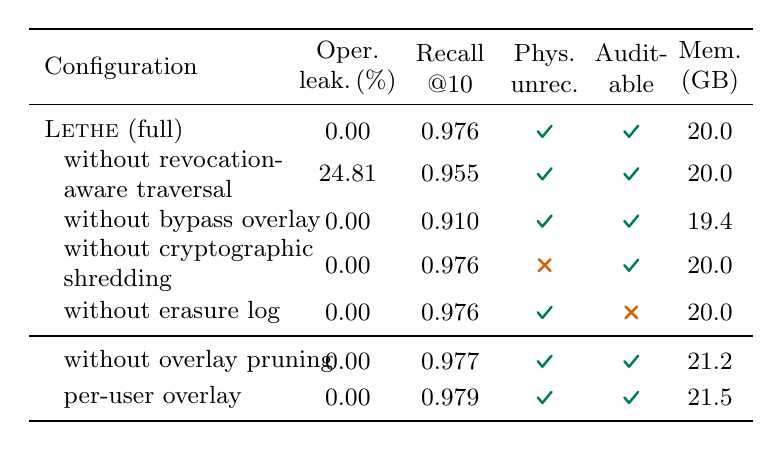
\begin{tikzpicture}[font=\small, inner sep=1pt]
  \def\xL{-0.15}\def\xR{9.05}
  \def\cx{3.9}\def\dx{5.2}\def\ex{6.4}\def\fx{7.5}\def\gx{8.5}
  % booktabs-style rules
  \draw[line width=0.9pt]  (\xL,0.50)  -- (\xR,0.50);
  \draw[line width=0.45pt] (\xL,-0.46) -- (\xR,-0.46);
  \draw[line width=0.45pt] (\xL,-3.40) -- (\xR,-3.40);
  \draw[line width=0.9pt]  (\xL,-4.48) -- (\xR,-4.48);
  % header: narrow 2-line abbreviated titles
  \node[anchor=west] at (0,0) {Configuration};
  \node[align=center] at (\cx,0) {Oper.\\leak.\,(\%)};
  \node[align=center] at (\dx,0) {Recall\\@10};
  \node[align=center] at (\ex,0) {Phys.\\unrec.};
  \node[align=center] at (\fx,0) {Audit-\\able};
  \node[align=center] at (\gx,0) {Mem.\\(GB)};
  % row 1
  \node[anchor=west] at (0,-0.80) {\textsc{Lethe} (full)};
  \node at (\cx,-0.80){0.00};  \node at (\dx,-0.80){0.976}; \node at (\ex,-0.80){\cmark}; \node at (\fx,-0.80){\cmark}; \node at (\gx,-0.80){20.0};
  % row 2 (wrapped label)
  \node[anchor=west,align=left] at (0.25,-1.34) {without revocation-\\aware traversal};
  \node at (\cx,-1.34){24.81}; \node at (\dx,-1.34){0.955}; \node at (\ex,-1.34){\cmark}; \node at (\fx,-1.34){\cmark}; \node at (\gx,-1.34){20.0};
  % row 3
  \node[anchor=west] at (0.25,-1.94) {without bypass overlay};
  \node at (\cx,-1.94){0.00};  \node at (\dx,-1.94){0.910}; \node at (\ex,-1.94){\cmark}; \node at (\fx,-1.94){\cmark}; \node at (\gx,-1.94){19.4};
  % row 4 (wrapped label)
  \node[anchor=west,align=left] at (0.25,-2.50) {without cryptographic\\shredding};
  \node at (\cx,-2.50){0.00};  \node at (\dx,-2.50){0.976}; \node at (\ex,-2.50){\xmark}; \node at (\fx,-2.50){\cmark}; \node at (\gx,-2.50){20.0};
  % row 5
  \node[anchor=west] at (0.25,-3.10) {without erasure log};
  \node at (\cx,-3.10){0.00};  \node at (\dx,-3.10){0.976}; \node at (\ex,-3.10){\cmark}; \node at (\fx,-3.10){\xmark}; \node at (\gx,-3.10){20.0};
  % row 6
  \node[anchor=west] at (0.25,-3.72) {without overlay pruning};
  \node at (\cx,-3.72){0.00};  \node at (\dx,-3.72){0.977}; \node at (\ex,-3.72){\cmark}; \node at (\fx,-3.72){\cmark}; \node at (\gx,-3.72){21.2};
  % row 7
  \node[anchor=west] at (0.25,-4.18) {per-user overlay};
  \node at (\cx,-4.18){0.00};  \node at (\dx,-4.18){0.979}; \node at (\ex,-4.18){\cmark}; \node at (\fx,-4.18){\cmark}; \node at (\gx,-4.18){21.5};
\end{tikzpicture}%
}
\end{table}

Table~\ref{tab:ablation} removes each one in turn, and each forfeits
exactly the axis it secures and no other: without revocation-aware traversal,
operational leakage returns to $24.8\%$ while recoverability and
auditability are untouched; without the bypass overlay, leakage stays at zero
but recall falls; without cryptographic shredding, the
revoked bytes become recoverable from a snapshot; and without the erasure log,
no revocation can be proven after the fact. The six axes are thus a
decomposition, not a list: no mechanism does two jobs and none is redundant.\ifextended\ Appendix~\ref{app:ablation} extends the ablation with the overlay construction and scope variants.\fi
The last two rows show why \textsc{Lethe} shares the overlay across
principals with the same effective view rather than materializing it per
user: the shared overlay is small ($0.6$ GB, $3\%$ of the index), but a
per-user overlay roughly triples it and raises total memory by about
$7\%$. Sharing is what keeps \textsc{Lethe}'s per-view erasure at
$1.26\times$ the base graph (\S\ref{sec:eval-cost}).

\section{Related Work}
\label{sec:related}

\paragraph{Streaming index maintenance.}
A large body of work keeps a graph or inverted index fresh under insertions
and deletions. Fresh\-Disk\-ANN~\cite{DBLP:journals/corr/abs-2105-09613} and
SPFresh~\cite{DBLP:conf/sosp/XuLLXCZLYYYCY23} consolidate deletions in the
background; incremental IVF maintenance~\cite{DBLP:journals/corr/abs-2411-00970},
proximity-graph maintenance~\cite{DBLP:journals/corr/abs-2206-10839},
real-time HNSW updates that repair unreachable
points~\cite{DBLP:journals/corr/abs-2407-07871}, in-place graph-index
updates~\cite{DBLP:journals/corr/abs-2502-13826}, and topology-aware
localized updates~\cite{DBLP:journals/pvldb/YuLGXLZSZLY25} each reduce the
recall and latency cost of churn. All score a
deletion by whether recall recovers. None asks whether a deleted vector still
steers traversal, whether its bytes survive, or whether the effect can be
confined to one view, the questions a revocation raises and \textsc{Lethe}
answers.

\paragraph{Access-controlled vector search.}
Filtering and partitioning systems enforce who may retrieve a vector.
ACORN~\cite{DBLP:journals/pacmmod/PatelKGZ24} and
Filtered-DiskANN~\cite{DBLP:conf/www/GollapudiKSKBRL23} attach predicates to
graph search; HoneyBee~\cite{DBLP:journals/corr/abs-2505-01538} and
Curator~\cite{DBLP:journals/corr/abs-2401-07119} partition by role or tenant;
production systems such as Milvus~\cite{DBLP:conf/sigmod/WangYGJXLWGLXYY21}
and Manu~\cite{DBLP:journals/pvldb/GuoLXYYLCXLLCQW22} expose row-level
security in the spirit of query rewriting~\cite{DBLP:conf/sigmod/RizviMSR04},
and zero-trust memory architectures~\cite{DBLP:journals/corr/abs-2601-07004}
carry the model into agent memory. Every one enforces the results
axis but not the routing or physical axes: \S\ref{sec:eval-exists} shows a revoked vector
still steering traversal under ACORN and HoneyBee, as it must under any
method that touches only the result. \textsc{Lethe} instead removes it from
traversal and storage, the routing and physical axes a result-level
filter leaves untouched. A complementary line protects the
confidentiality of the query or data rather than controlling who may see a
result. Private ANN search lets a client search without
revealing its query to the server: PACMANN~\cite{DBLP:conf/iclr/ZhouSF25}
retrieves graph neighborhoods by per-hop private information retrieval (PIR),
Panther~\cite{DBLP:conf/ccs/LiHZ0L0C25} combines PIR
with secret sharing and homomorphic encryption in a single-server setting, while
secure $k$-nearest-neighbor classification~\cite{DBLP:journals/popets/ShaulFR20}
and federated vector search across
organizations~\cite{DBLP:journals/pacmmod/ZhangWXPX24,DBLP:journals/pvldb/ZhuFZSXZD24,DBLP:journals/pvldb/FanZZT25} protect data split between
parties. Each adds cryptographic or communication cost to keep the query or
underlying data confidential, orthogonal to removing a revoked vector from a
shared plaintext index.

\paragraph{Leakage channels and inference control.}
Restricting what a system returns has long been known to fall short of stopping
disclosure. Statistical databases refusing to answer small query sets were
still compromised by \emph{trackers}, characteristic formulas that recover the
forbidden statistics~\cite{DBLP:journals/tods/DenningDS79,DBLP:journals/tods/DenningS80},
despite inference controls built to stop them~\cite{DBLP:journals/tods/Denning80};
multilevel and statistical databases leak through inference channels that
combine constraints with auxiliary
data~\cite{JajodiaMeadows95,DBLP:journals/sigkdd/FarkasJ02,DBLP:journals/tkde/BrodskyFJ00,DBLP:journals/tse/ChinO82};
and encrypted or outsourced databases leak through access patterns and
response volumes, which leakage-abuse and reconstruction attacks turn into
recovered queries and
records~\cite{DBLP:conf/ndss/IslamKK12,DBLP:conf/ccs/CashGPR15,DBLP:conf/ccs/NaveedKW15,DBLP:conf/ccs/KellarisKNO16,DBLP:conf/ccs/GrubbsLMP18,DBLP:conf/sp/GrubbsLMP19}.
The common thread is a side channel that outlives a result-level restriction.
Operational leakage is this phenomenon inside a graph index: a revoked vector
filtered from the answer still steers traversal, and the neighborhoods it shifts
are a side channel an adversary reads off (\S\ref{sec:eval-exists}). The stored bytes are not opaque either: embedding inversion
reconstructs source text from a vector alone; Morris et
al.~\cite{DBLP:conf/emnlp/MorrisKSR23} recover 92\% of 32-token inputs exactly
and extract full names from clinical notes given only vector-database access and
embedding pairs. \textsc{Lethe} therefore treats leakage as a property of
navigational structure and stored bytes rather than of the result set, closing
the routing channel with revocation-aware traversal and the content channel with
vector-granular cryptographic shredding, both held to per-view scope.

\paragraph{Secure deletion, unlearning, and the right to be forgotten.}
A separate line formalizes what deletion should mean. Secure-deletion systems
erase bytes from storage media~\cite{DBLP:conf/sp/ReardonBC13}; machine
unlearning removes a training example's influence from a
model~\cite{DBLP:conf/sp/CaoY15,DBLP:conf/sp/BourtouleCCJTZL21,DBLP:conf/nips/GinartGVZ19};
the right to be forgotten has a cryptographic
definition~\cite{DBLP:conf/eurocrypt/GargGV20}, and dependency-aware erasure
asks what else must go when one record
does~\cite{DBLP:journals/pvldb/ChakrabortyKMNNPSV25}, all driven by
regulation~\cite{GDPR16}. \textsc{Lethe} carries these guarantees where they
have not reached: into the navigational structure of a shared ANN index,
where deletion must also stop routing, hold to per-view scope, and take
effect at once.

\paragraph{Verifiable retrieval and inference privacy.}
V3DB proves vector-search results
against a committed snapshot with zero-knowledge
proofs~\cite{DBLP:journals/corr/abs-2603-03065}; \textsc{Lethe}'s
erasure log is a lighter append-only audit trail for revocations rather than
a per-query proof, and the two compose. Distinct again is the line
bounding what query answers reveal about the data through differential privacy
over selection and top-$k$~\cite{DBLP:conf/focs/McSherryT07,DBLP:conf/nips/DurfeeR19,DBLP:conf/icml/GillenwaterJMD22};
limiting inference about a present record is orthogonal to removing a
revoked one from a shared index, the problem we take up.

\section{Conclusion and Future Work}
\label{sec:conclusion}

A revoked vector filtered from every result can still steer the
search that produces it, remain recoverable on disk, and, when finally
removed, disturb users who never lost access. We named this the zombie vector
phenomenon, formalized per-view erasure over six axes, and showed that no
standard maintenance primitive achieves it. \textsc{Lethe} does, by moving
erasure out of the index structure and into the traversal and the keys:
revocation-aware traversal, an effective-view-shared bypass overlay,
cryptographic shredding, and an append-only erasure log, each closing exactly one
axis. Across four datasets, two graph indexes, and up to a billion
vectors, it drives operational leakage to zero, holds recall within half a
point of an oracle per-view rebuild, leaves unaffected views untouched, erases
immediately, and costs $1.26\times$ the base graph where a per-role index
costs $84\times$ at 100 roles.

Two assumptions bound these guarantees. Cryptographic shredding reduces
physical erasure to key destruction, inheriting the trust placed in the
key-management layer: a server that secretly retains key material defeats it,
as it would any such scheme. And the memory advantage
depends on permissions that overlap, since the bypass overlay is sized by the
number of distinct effective views; a workload in which almost every vector is private to one
principal drives it toward the per-user cost it otherwise avoids. Timing
results are single-machine trends, and we evaluate revocation rather than
wholesale changes to the lattice, whose overlay maintenance we leave to future
work.

The lesson outlives the system. In any shared structure that is navigated
rather than scanned, removing a record from the answers is not the same as
removing it from the system: the structure itself carries the record's
influence, and an access check at the output cannot reach it. Erasure has to
be a property of how the structure is traversed, not only of what it returns.

%% ==========================================================
%% BIBLIOGRAPHY  (IEEEtran numeric style, from the shared bib)
%% ==========================================================

\bibliographystyle{ACM-Reference-Format}
\bibliography{zombievectors}

\ifextended
\clearpage
\appendix
\emergencystretch=2em % gentle: avoid small hbox overfulls in dense two-column appendix proofs

\begin{strip}
\vspace*{0.3em}
\begin{center}{\large\bfseries Appendix Contents}\end{center}
\vspace{4pt}
\centering
\setlength{\tabcolsep}{10pt}
\renewcommand{\arraystretch}{1.2}
\begin{tabular}{@{}p{0.46\textwidth}p{0.46\textwidth}@{}}
\toprule
\hyperref[app:formal]{\textbf{\ref*{app:formal}}\hspace{0.5em}\textbf{Extended Formalism and Proofs}} & \hspace*{1.2em}\hyperref[app:suite-recall]{\ref*{app:suite-recall}\hspace{0.5em}Recall across the revocation sweep} \\
\hspace*{1.2em}\hyperref[app:model]{\ref*{app:model}\hspace{0.5em}Notation and model} & \hspace*{1.2em}\hyperref[app:diskann]{\ref*{app:diskann}\hspace{0.5em}Generality to a second graph index (DiskANN/Vamana)} \\
\hspace*{1.2em}\hyperref[app:axes]{\ref*{app:axes}\hspace{0.5em}The six axes, formally} & \hspace*{1.2em}\hyperref[app:crash]{\ref*{app:crash}\hspace{0.5em}Concurrency and crash consistency} \\
\hspace*{1.2em}\hyperref[app:imposs]{\ref*{app:imposs}\hspace{0.5em}No standard primitive achieves per-view erasure} & \hspace*{1.2em}\hyperref[app:exception]{\ref*{app:exception}\hspace{0.5em}Sensitivity to the predicate exception rate} \\
\hspace*{1.2em}\hyperref[app:correct]{\ref*{app:correct}\hspace{0.5em}Correctness of \textsc{Lethe}} & \hspace*{1.2em}\hyperref[app:samerole]{\ref*{app:samerole}\hspace{0.5em}User-level revocation within a shared role} \\
\hspace*{1.2em}\hyperref[app:cost]{\ref*{app:cost}\hspace{0.5em}Complexity and cost} & \hspace*{1.2em}\hyperref[app:viewscope]{\ref*{app:viewscope}\hspace{0.5em}Scope of the disturbance to unaffected users} \\
\hspace*{1.2em}\hyperref[app:scope]{\ref*{app:scope}\hspace{0.5em}Assumptions, threat model, and scope} & \hyperref[app:ablation]{\textbf{\ref*{app:ablation}}\hspace{0.5em}\textbf{Ablation of the bypass overlay}} \\
\hyperref[app:repro]{\textbf{\ref*{app:repro}}\hspace{0.5em}\textbf{Reproducibility}} & \hyperref[app:security]{\textbf{\ref*{app:security}}\hspace{0.5em}\textbf{Adversarial and security evaluation}} \\
\hspace*{1.2em}\hyperref[app:repro-data]{\ref*{app:repro-data}\hspace{0.5em}Datasets and access-control workload} & \hspace*{1.2em}\hyperref[app:sec-attacks]{\ref*{app:sec-attacks}\hspace{0.5em}Inference attacks} \\
\hspace*{1.2em}\hyperref[app:repro-build]{\ref*{app:repro-build}\hspace{0.5em}Index construction and operating point} & \hspace*{1.2em}\hyperref[app:sec-adv]{\ref*{app:sec-adv}\hspace{0.5em}Adversarial revocation targeting} \\
\hspace*{1.2em}\hyperref[app:repro-methods]{\ref*{app:repro-methods}\hspace{0.5em}Methods} & \hspace*{1.2em}\hyperref[app:sec-phys]{\ref*{app:sec-phys}\hspace{0.5em}Physical unrecoverability} \\
\hspace*{1.2em}\hyperref[app:repro-metrics]{\ref*{app:repro-metrics}\hspace{0.5em}Revocation workloads and metrics} & \hspace*{1.2em}\hyperref[app:sec-audit]{\ref*{app:sec-audit}\hspace{0.5em}Audit tamper-evidence} \\
\hspace*{1.2em}\hyperref[app:repro-stats]{\ref*{app:repro-stats}\hspace{0.5em}Statistical protocol} & \hyperref[app:stats]{\textbf{\ref*{app:stats}}\hspace{0.5em}\textbf{Statistical significance}} \\
\hspace*{1.2em}\hyperref[app:repro-manifest]{\ref*{app:repro-manifest}\hspace{0.5em}Data artifact manifest} & \hyperref[app:microtrace]{\textbf{\ref*{app:microtrace}}\hspace{0.5em}\textbf{Micro-trace of a single query}} \\
\hyperref[app:baseline]{\textbf{\ref*{app:baseline}}\hspace{0.5em}\textbf{Complete baseline comparison}} & \hyperref[app:limits]{\textbf{\ref*{app:limits}}\hspace{0.5em}\textbf{Limitations}} \\
\hspace*{1.2em}\hyperref[app:baseline-perds]{\ref*{app:baseline-perds}\hspace{0.5em}Per-dataset breakdown} & \hspace*{1.2em}\hyperref[app:limits-scope]{\ref*{app:limits-scope}\hspace{0.5em}Scope boundaries} \\
\hyperref[app:suite]{\textbf{\ref*{app:suite}}\hspace{0.5em}\textbf{Experiment suite: drift and recall across the revocation sweep}} & \hspace*{1.2em}\hyperref[app:limits-emp]{\ref*{app:limits-emp}\hspace{0.5em}Empirical and methodological boundaries} \\
\bottomrule
\end{tabular}
\vspace{6pt}
\end{strip}

\section{Extended Formalism and Proofs}
\label{app:formal}

This appendix consolidates the formal model of
\S\ref{sec:background}--\S\ref{sec:query}, completes the proofs the body
defers, and gives the complexity analysis behind its asymptotic claims. All
notation is that of the body; Table~\ref{tab:symbols} collects it in one
place. We fix the model (\S\ref{app:model}), restate the six axes as formal
predicates (\S\ref{app:axes}), give the full impossibility argument
(\S\ref{app:imposs}), prove that \textsc{Lethe} achieves per-view erasure
(\S\ref{app:correct}), analyze its cost (\S\ref{app:cost}), and state the
assumptions and scope of the guarantees (\S\ref{app:scope}).

\subsection{Notation and model}
\label{app:model}

\subsubsection{Index and graph.}
A graph vector index is a pair $\mathcal{I}=(G,S)$. The \emph{navigable graph}
$G=(P,E)$ is a directed graph over a dataset
$P=\{p_1,\dots,p_N\}\subset\mathbb{R}^d$ of $N$ vectors in $d$ dimensions;
each node $p$ stores an adjacency list of out-neighbors $\Nout(p)$ capped at
an out-degree bound $M$, and we write $\Nin(p)=\{p'\in P: p\in\Nout(p')\}$ for
its in-neighbors. The \emph{physical store} $S$ holds the bytes of every
$p\in P$. The graph is \emph{navigable} when, from a fixed entry point
$\mathit{ep}$, greedy descent reaches the neighborhood of a query in a few
hops, which requires that the nodes along the way carry edges toward
it~\cite{DBLP:journals/pami/MalkovY20,DBLP:conf/nips/SubramanyaDSKK19}.

\subsubsection{Search semantics.}
\label{app:search-sem}
A query $q$ for principal $u$ is answered by greedy best-first traversal
(Alg.~\ref{alg:search}). The search keeps a frontier $W$ of the $\mathit{ef}$
candidates nearest $q$ seen so far; it repeatedly expands the closest
unexpanded candidate by visiting its out-neighbors, and stops when $W$ no
longer improves. We write $\mathrm{Visit}(\mathcal{I},q,u)\subseteq P$ for the
set of nodes \emph{expanded} during this traversal and
$\mathrm{Ans}(\mathcal{I},q,u)$ for the $k$ visited nodes nearest $q$ that are
returned; both are the principal-aware forms of $\mathrm{Visit}(q,G)$ and
$R_k(q,G)$ from \S\ref{sec:background}. Quality is measured against the exact
neighbors $\mathrm{NN}_k(q)$ by
$\mathrm{Recall}@k=|\mathrm{Ans}(\mathcal{I},q,u)\cap\mathrm{NN}_k(q)\cap
P_u|/k$, the fraction of the true $k$ nearest \emph{authorized} neighbors
recovered.

For a fixed run on $(q,u)$ we attach to each node $p$ six monotone event
predicates that record how far $p$ participates in the traversal; they make
the informal stages of \S\ref{sec:background} and the leakage instrumentation
of \S\ref{sec:eval} precise.
\begin{itemize}
\item $\mathsf{enc}(p)$: $p$'s identifier is \emph{encountered}, i.e.\ it
  appears in an adjacency list the search scans.
\item $\mathsf{chk}(p)$: the access predicate $u\in A(p)$ is \emph{evaluated}
  for $p$.
\item $\mathsf{scr}(p)$: $p$ is \emph{distance-scored}, i.e.\ its distance to
  $q$ is computed.
\item $\mathsf{ins}(p)$: $p$ is \emph{inserted} into the frontier $W$.
\item $\mathsf{exp}(p)$: $p$ is \emph{expanded}; equivalently
  $p\in\mathrm{Visit}(\mathcal{I},q,u)$.
\item $\mathsf{ret}(p)$: $p$ is \emph{returned}; equivalently
  $p\in\mathrm{Ans}(\mathcal{I},q,u)$.
\end{itemize}
These hold in the order
$\mathsf{ret}(p)\Rightarrow\mathsf{exp}(p)\Rightarrow\mathsf{ins}(p)
\Rightarrow\mathsf{scr}(p)\Rightarrow\mathsf{chk}(p)\Rightarrow\mathsf{enc}(p)$:
a node cannot be returned without having been expanded, expanded without
having entered the frontier, and so on. We call $p$ a \emph{routing waypoint}
for $(q,u)$ when $\mathsf{exp}(p)$ holds, and we say $p$ \emph{participates} in
the traversal when $\mathsf{scr}(p)\lor\mathsf{ins}(p)\lor\mathsf{exp}(p)
\lor\mathsf{ret}(p)$ holds. As the body's footnote to Table~\ref{tab:axes}
notes, $\mathsf{enc}(p)$ alone is benign: $p$ may sit in the adjacency list of
a node still shared with views that hold it, so its identifier can be
encountered without $p$ participating.

\subsubsection{Access-control model.}
\label{app:access}
A shared index serves a set of principals $U$ (users or roles). An access
policy assigns each vector $p$ an authorized set $A(p)\subseteq U$; principal
$u$'s \emph{view} is the sub-dataset $P_u=\{p\in P:u\in A(p)\}$ it may
retrieve. Permissions form a lattice $(L,\sqsubseteq)$ of roles, where
$\ell'\sqsubseteq\ell$ means role $\ell$ subsumes (\emph{dominates}) the access
of $\ell'$. Each principal $u$ holds a role $\lambda(u)\in L$ and each vector
$p$ is tagged with the least role $\lambda(p)\in L$ permitted to see it, so
$u$ may retrieve $p$ exactly when $\lambda(p)\sqsubseteq\lambda(u)$, i.e.\
$A(p)=\{u\in U:\lambda(p)\sqsubseteq\lambda(u)\}$. For a role $\ell\in L$ we
write $P_\ell=\{p\in P:\lambda(p)\sqsubseteq\ell\}$ for the vectors visible at
$\ell$; a principal's view is the view of its role, $P_u=P_{\lambda(u)}$, so
principals sharing a role share a view.

A principal's \emph{effective view} is $P_u$ once individual exceptions are
applied. Principals with the same effective view form an \emph{effective-view
class}; we write $\mathrm{ev}(u)$ for the class of $u$, which is its role
$\lambda(u)$ when no individual exception applies and a refinement of it
otherwise. The access test is realized by storing, with each $p$, its role tag
$\lambda(p)$ and a short \emph{exception list} of principals revoked from the
role-induced default; $u\in A(p)$ then checks $\lambda(p)\sqsubseteq\lambda(u)$
against a precomputed reachability relation on $L$ and consults the exception
list, in $O(1)$ (\S\ref{sec:ds}, formalized in \S\ref{app:cost}).

\subsubsection{Erasure requests and the reference view.}
\label{app:requests}
\begin{sloppypar}
A \emph{revocation} $\rev(u,p)$ removes $u$ from $A(p)$, shrinking $P_u$ by
one vector and leaving $P_{u'}$ unchanged for every other principal. An
\emph{erasure request} $\rho=(p,R)$ names a vector $p$ and a scope
$R\subseteq U$ of principals who must lose access to it: $R=\{u\}$ is a single
revocation and $R=U$ is \emph{global erasure}. Applying $\rho$ transforms
$\mathcal{I}=(G,S)$ into $\mathcal{I}'=(G',S')$ with $u\notin A(p)$, hence
$p\notin P_u$, for every $u\in R$. We write $\mathcal{L}(R)$ for the set of
effective-view classes whose view loses $p$ under $\rho$: one class for a
single-role revocation, the class $\mathrm{ev}(u)$ for $R=\{u\}$, and every
class whose view contained $p$ for $R=U$.
\end{sloppypar}

To say what $u$ \emph{should} observe once $p$ leaves its view, we fix a
reference $\mathcal{I}^\star_u$, the index built on exactly $P_u$ -- the oracle
per-view rebuild of \S\ref{sec:phenomenon}, the behavior an index would have
if $p$, and every other vector $u$ cannot see, had never been inserted for
$u$. The reference is an empirical quality target, not part of the guarantee:
Definition~\ref{def:pve} pins down $p$'s operational non-participation exactly,
while \S\ref{sec:eval} shows the resulting answers track $\mathcal{I}^\star_u$
to within its own seed-to-seed variation.

\begin{table*}[t]
\centering
\caption{Symbols used in the body and this appendix, with the section of first
use. Notation is identical throughout; the event predicates of
\S\ref{app:search-sem} make the leakage stages of \S\ref{sec:eval} precise.}
\label{tab:symbols}
\small
\renewcommand{\arraystretch}{1.18}
\begin{tabular}{@{}l l l@{}}
\toprule
Symbol & Meaning & First use \\
\midrule
$\mathcal{I}=(G,S)$ & Index: navigable graph $G$ and physical store $S$ & \S\ref{sec:background},~\S\ref{sec:formal} \\
$P=\{p_1,\dots,p_N\}$ & Dataset of $N$ vectors in $\mathbb{R}^d$ & \S\ref{sec:background} \\
$G=(P,E)$ & Directed navigable graph over $P$ & \S\ref{sec:background} \\
$\Nout(p),\ \Nin(p)$ & Out- and in-neighbors of node $p$ & \S\ref{sec:background} \\
$M$ & Out-degree bound & \S\ref{sec:background} \\
$\mathit{ep},\ \mathit{ef}$ & Entry point; frontier width & \S\ref{sec:background},~\S\ref{sec:query} \\
$W$ & Frontier of authorized candidates during search & \S\ref{sec:query} \\
$\mathrm{Visit}(\mathcal{I},q,u)$ & Nodes expanded for query $q$, principal $u$ & \S\ref{sec:formal} \\
$\mathrm{Ans}(\mathcal{I},q,u)$ & Top-$k$ returned over $u$'s view & \S\ref{sec:formal} \\
$R_k(q,G)$ & $k$ returned neighbors (view-agnostic form) & \S\ref{sec:background} \\
$\mathrm{NN}_k(q)$ & Exact $k$ nearest neighbors of $q$ & \S\ref{sec:background} \\
$\mathrm{Recall}@k$ & Fraction of authorized true neighbors recovered & \S\ref{sec:background} \\
$\mathsf{enc},\mathsf{chk},\mathsf{scr}$ & Encountered / predicate-checked / distance-scored & \S\ref{app:search-sem} \\
$\mathsf{ins},\mathsf{exp},\mathsf{ret}$ & Frontier-inserted / expanded / returned & \S\ref{app:search-sem} \\
$U$ & Set of principals (users or roles) & \S\ref{sec:background} \\
$A(p)$ & Authorized set of $p$ (access predicate) & \S\ref{sec:background},~\S\ref{sec:design} \\
$P_u,\ P_\ell$ & View of principal $u$; vectors visible at role $\ell$ & \S\ref{sec:background} \\
$(L,\sqsubseteq)$ & Permission lattice of roles & \S\ref{sec:background} \\
$\lambda(u),\ \lambda(p)$ & Role of principal $u$; least role tagging $p$ & \S\ref{sec:background} \\
$\mathrm{ev}(u)$ & Effective-view class of $u$ & \S\ref{sec:query} \\
$\rev(u,p)$ & Revocation: remove $u$ from $A(p)$ & \S\ref{sec:background} \\
$\rho=(p,R)$ & Erasure request: vector $p$, scope $R\subseteq U$ & \S\ref{sec:formal} \\
$\mathcal{L}(R)$ & Effective-view classes whose view loses $p$ & \S\ref{sec:query} \\
$\mathcal{I}^\star_u$ & Oracle reference index built on exactly $P_u$ & \S\ref{sec:formal} \\
$\mathrm{Bypass}_\ell(a)$ & Bypass edges of $a$ tagged class $\ell$ & \S\ref{sec:query} \\
$\mathrm{Prune}(x,\mathit{cand},M)$ & Robust neighbor-selection heuristic & \S\ref{sec:design} \\
\bottomrule
\end{tabular}
\end{table*}

\subsection{The six axes, formally}
\label{app:axes}

Table~\ref{tab:axes} states each axis as a condition on the post-request index
$\mathcal{I}'$. We restate the six as formal predicates over the event
predicates of \S\ref{app:search-sem}, so that the impossibility argument
(\S\ref{app:imposs}) and the correctness proof (\S\ref{app:correct}) reduce to
checking them. Fix a request $\rho=(p,R)$ taking $\mathcal{I}=(G,S)$ to
$\mathcal{I}'=(G',S')$.

\subsubsection{The axis predicates.}
\label{app:axis-preds}
\begin{description}
\item[\textsc{Results}.] For every $u\in R$ and every query $q$,
  $p\notin\mathrm{Ans}(\mathcal{I}',q,u)$; equivalently $\lnot\mathsf{ret}(p)$
  on every run $(q,u)$ with $u\in R$.
\item[\textsc{Routing}.] For every $u\in R$ and every query $q$, $p$ does not
  \emph{participate}: $\lnot\big(\mathsf{scr}(p)\lor\mathsf{ins}(p)\lor
  \mathsf{exp}(p)\lor\mathsf{ret}(p)\big)$. In particular
  $p\notin\mathrm{Visit}(\mathcal{I}',q,u)$. The benign event $\mathsf{enc}(p)$
  is permitted, since $p$ may remain a physical node shared with views that
  still hold it (footnote to Table~\ref{tab:axes}).
\item[\textsc{Physical}.] If $R=U$, then $p$'s bytes are unrecoverable from
  $S'$: there is no efficient procedure that, given read access to live memory
  and to every serialized snapshot of $S'$, outputs $p$'s plaintext (formalized
  under stated assumptions in \S\ref{app:correct-phys}).
\item[\textsc{Immediate}.] The \textsc{Results} and \textsc{Routing}
  predicates hold for every query accepted at or after the time $\rho$ is
  accepted; there is a single instant (the linearization point of
  \S\ref{app:correct-imm}) before which $\rho$ has no effect and after which
  both hold.
\item[\textsc{Verifiable}.] There is a tamper-evident record $\tau(\rho)$ such
  that a third party holding the public verification state can confirm $\rho$
  was issued and ordered, and any alteration of the recorded history is
  detected (formalized in \S\ref{app:correct-ver}).
\item[\textsc{View-scope}.] For every $u'\notin R$ with $p\in P_{u'}$, the run
  $(q,u')$ is unchanged in its answer and in $p$'s participation: $p\in
  \mathrm{Ans}(\mathcal{I}',q,u')\iff p\in\mathrm{Ans}(\mathcal{I},q,u')$, and
  likewise for $\mathsf{exp}(p)$; and $u'$ keeps its recall up to the
  seed-level drift measured in \S\ref{sec:eval}.
\end{description}

\begin{definition}[Per-view erasure; restatement of Definition~\ref{def:pve}]
\label{def:pve-app}
A mechanism achieves \emph{per-view erasure} if, for every request
$\rho=(p,R)$, the index $\mathcal{I}'$ it produces satisfies
\textsc{Results}, \textsc{Routing}, \textsc{Immediate}, \textsc{Verifiable},
and \textsc{View-scope} for scope $R$, and additionally \textsc{Physical} when
$R=U$.
\end{definition}

\subsubsection{Routing is strictly stronger than Results.}
\label{app:routing-results}
The body keeps \textsc{Results} and \textsc{Routing} separate because they are
not equivalent; we make the implication and its failure precise.

\begin{lemma}[\textsc{Routing} implies \textsc{Results}]
\label{lem:routing-results}
For any index and any scope $R$, if $\mathcal{I}'$ satisfies \textsc{Routing}
for $\rho=(p,R)$ then it satisfies \textsc{Results} for $\rho$.
\end{lemma}
\begin{proof}
By the ordering of \S\ref{app:search-sem}, $\mathsf{ret}(p)\Rightarrow
\mathsf{exp}(p)$, so $\mathsf{ret}(p)$ implies $p$ participates. \textsc{Routing}
forbids participation for every $u\in R$ and every $q$, hence forbids
$\mathsf{ret}(p)$, which is exactly \textsc{Results}.
\end{proof}

\begin{lemma}[\textsc{Results} does not imply \textsc{Routing}]
\label{lem:results-not-routing}
There is an index, a request $\rho=(p,R)$, and a query $q$ for which
$\mathcal{I}'$ satisfies \textsc{Results} but violates \textsc{Routing}.
\end{lemma}
\begin{proof}
Take the running example of Fig.~\ref{fig:example}, in which the bridge $b$
lies on the greedy path to $q$ -- $\mathsf{exp}(b)$ holds -- yet $b\notin
R_k(q,G)$, so $\mathsf{ret}(b)$ does not. Let $\rho=(b,\{u\})$ and let
$\mathcal{I}'$ be produced by a mechanism that filters $b$ from the answer but
leaves it a node of $G'$ with its edges intact (the Tombstone behavior of
\S\ref{sec:phenomenon}). Then $\lnot\mathsf{ret}(b)$ on $(q,u)$, so
\textsc{Results} holds, while $\mathsf{exp}(b)$ still holds, so $b$
participates and \textsc{Routing} fails. The participation of $b$ moves the
frontier and can change which other vectors are returned: this is the zombie
channel whose drift \S\ref{sec:phenomenon} measures.
\end{proof}

Lemmas~\ref{lem:routing-results}--\ref{lem:results-not-routing} place
\textsc{Routing} strictly above \textsc{Results} in the order of guarantees:
an access check applied only at the output enforces the latter but never the
former.

\subsubsection{Per-view leakage.}
\label{app:leakage}
Definition~\ref{def:pve-app} drives to zero the extent to which $p$ still
reaches a revoked view. We name that quantity. For a request $\rho=(p,R)$, a
revoked principal $u\in R$, and a distribution $\mathcal{Q}$ over queries,
define the \emph{per-view leakage}
\[
  \mathrm{Leak}(p,u)=\Pr_{q\sim\mathcal{Q}}\!\big[\,\mathsf{scr}(p)\lor
  \mathsf{ins}(p)\lor\mathsf{exp}(p)\lor\mathsf{ret}(p)\ \text{on run }(q,u)\,\big],
\]
the probability that $p$ participates in the traversal of a query issued by
$u$ after revocation. Summing the disjuncts by stage gives the stage-resolved
leakage, scored, frontier, expanded, and returned (result) leakage, that
\S\ref{sec:eval} reports and the instrumentation of
\S\ref{sec:eval} records per query; \emph{operational leakage} is the expanded
component, the rate at which a revoked vector is still a routing waypoint.

\begin{proposition}
\label{prop:leak-zero}
A mechanism satisfies \textsc{Results} and \textsc{Routing} for $\rho=(p,R)$
if and only if $\mathrm{Leak}(p,u)=0$ for every $u\in R$ and every query
distribution $\mathcal{Q}$.
\end{proposition}
\begin{proof}
\textsc{Routing} forbids each disjunct in the definition of
$\mathrm{Leak}$ for every $u\in R$ and every $q$, so the probability is $0$
under any $\mathcal{Q}$; with Lemma~\ref{lem:routing-results} this also gives
\textsc{Results}. Conversely, if $\mathrm{Leak}(p,u)=0$ for every $\mathcal{Q}$
then, choosing $\mathcal{Q}$ to be the point mass at an arbitrary $q$, no
disjunct holds on $(q,u)$; as this is exactly the participation of $p$,
\textsc{Routing} holds, and \textsc{Results} follows.
\end{proof}

This is a structural property of the index: it bounds $p$'s operational
participation, and is separate from inference about hidden data from public
structure, which we do not study (\S\ref{app:scope}).

\subsubsection{The axes are independent.}
\label{app:independence}
The body calls the six axes independent. We make this precise: no axis is
implied by the conjunction of the others, so none is redundant.

\begin{proposition}
\label{prop:independence}
For each of the six axes there is a mechanism that satisfies the other five
(on the requests where they apply) but violates it. Hence the six are
logically independent, and Definition~\ref{def:pve-app} is not implied by any
five of its conjuncts.
\end{proposition}
\begin{proof}
We exhibit a witness per axis; the per-primitive analysis of
\S\ref{app:imposs} and the matrix of Fig.~\ref{fig:matrix} supply the
behaviors invoked.

\emph{Routing.} A mechanism that filters $p$ from answers, audits the
revocation, scopes it to $R$, and crypto-shreds at $R=U$, but leaves $p$
routing, satisfies all axes except \textsc{Routing}
(Lemma~\ref{lem:results-not-routing}).

\emph{Results.} Returning $p$ while otherwise erasing it is precluded by
Lemma~\ref{lem:routing-results} only when \textsc{Routing} holds; a mechanism
that suppresses participation in scoring, expansion, and the frontier but
admits $p$ into the final answer set by a separate output path violates
\textsc{Results} alone. Such a mechanism is degenerate but well defined,
witnessing that \textsc{Results} is not implied by the rest.

\emph{Physical.} \textsc{Lethe} without cryptographic shredding
(\S\ref{sec:eval}, ablation) satisfies every axis but, at $R=U$, leaves $p$'s
bytes in the live store, violating \textsc{Physical}.

\emph{Immediate.} A mechanism that defers the predicate flip and bypass to a
periodic pass attains all axes once it runs but violates \textsc{Immediate}
until then (the Periodic-rebuild behavior).

\emph{Verifiable.} \textsc{Lethe} without the erasure log satisfies every
operational axis but produces no tamper-evident record, violating
\textsc{Verifiable}.

\emph{View-scope.} A global physical deletion attains \textsc{Results},
\textsc{Routing}, \textsc{Physical}, and \textsc{Immediate} but removes $p$
for every principal, violating \textsc{View-scope}.

Each axis thus has a witness satisfying the other five, so none follows from
their conjunction.
\end{proof}

Proposition~\ref{prop:independence} is the formal content behind the empty and
filled cells of Fig.~\ref{fig:matrix}: each prior method occupies a distinct
pattern of satisfied axes, and only their conjunction, which no single
mechanism in the figure attains, is per-view erasure.

\subsection{No standard primitive achieves per-view erasure}
\label{app:imposs}

Theorem~\ref{thm:sixaxis} states that none of the standard maintenance
primitives, applied alone, achieves per-view erasure. The body gives the
argument in prose; here we prove one lemma per primitive against the formal
predicates of \S\ref{app:axis-preds}, then draw the two structural
conclusions that motivate \textsc{Lethe} (\S\ref{app:imposs-cor}). Throughout,
$\rho=(p,R)$ is an erasure request and $\mathcal{I}'$ the index the primitive
produces; Fig.~\ref{fig:matrix} records the full pattern of satisfied axes.

\subsubsection{Per-primitive lemmas.}
\label{app:imposs-lemmas}

\begin{lemma}[Tombstone]
\label{lem:tombstone}
Tombstone satisfies \textsc{Results} and \textsc{Immediate} but violates
\textsc{Routing}, \textsc{Physical}, \textsc{Verifiable}, and
\textsc{View-scope}.
\end{lemma}
\begin{proof}
Tombstone sets a deleted flag on $p$ and filters flagged nodes from the
returned set, so $\lnot\mathsf{ret}(p)$ on every run: \textsc{Results} holds,
and because the flag is read live it holds from the next query
(\textsc{Immediate}). But $p$ remains a node of $G'$ with $\Nout(p)$ and
$\Nin(p)$ intact; nothing in the traversal consults a per-view predicate, so
$p$ is still distance-scored, inserted, and expanded on a revoked user's
query. Thus $\mathsf{exp}(p)$ holds, $p$ participates, and \textsc{Routing}
fails (the drift this induces is measured in \S\ref{sec:phenomenon}). The
bytes of $p$ stay in the live store and in every snapshot, so for $R=U$ they
remain recoverable: \textsc{Physical} fails. A mutable flag is not a
tamper-evident record: \textsc{Verifiable} fails. And the flag is global, it suppresses $p$ for every principal at once, with no dependence on $R$, so a request $R=\{u\}$ also denies $p$ to principals $u'\neq u$ that should
keep it: \textsc{View-scope} fails.
\end{proof}

\begin{lemma}[Physical-delete]
\label{lem:physdelete}
Physical-delete satisfies \textsc{Results}, \textsc{Routing}, \textsc{Physical},
and \textsc{Immediate} but violates \textsc{Verifiable} and \textsc{View-scope}.
\end{lemma}
\begin{proof}
Physical-delete removes $p$'s node from $G'$ and repairs its in-neighbors
$\Nin(p)$ by re-pointing them to suitable survivors. After it runs, $p$ is no
node of $G'$, so no event predicate beyond $\mathsf{enc}$ can fire: $p$ is
neither scored, expanded, nor returned, giving \textsc{Routing} and
\textsc{Results}; its bytes are gone from the live store, giving
\textsc{Physical} for $R=U$; and the in-place edit takes effect at once
(\textsc{Immediate}). But the deletion acts on the single shared graph, hence
on every principal regardless of $R$: a request $R=\{u\}$ removes $p$ from
$P_{u'}$ for $u'\neq u$ that still hold it, so \textsc{View-scope} fails. And
the edit leaves no auditable artifact attesting the request occurred:
\textsc{Verifiable} fails.
\end{proof}

\begin{lemma}[Periodic-rebuild]
\label{lem:rebuild}
Periodic-rebuild satisfies \textsc{Results} and \textsc{Routing} once it runs
but violates \textsc{Physical}, \textsc{Immediate}, \textsc{Verifiable}, and
\textsc{View-scope}.
\end{lemma}
\begin{proof}
At the next scheduled pass, Periodic-rebuild reconstructs the graph on the
surviving set, after which $p$ is absent and neither routes nor appears in any
answer (\textsc{Routing}, \textsc{Results}). But the pass is deferred: between
acceptance of $\rho$ and the next rebuild, $p$ stays a node of the live graph
and store, so it keeps routing and its bytes stay recoverable. Hence
\textsc{Immediate} fails, and for $R=U$ \textsc{Physical} fails during the
entire compliance window of \S\ref{sec:phenomenon}. The rebuild is over the
single shared set, so it is global (\textsc{View-scope} fails), and it
produces no tamper-evident record of the request (\textsc{Verifiable} fails).
\end{proof}

\begin{lemma}[Cryptographic shredding]
\label{lem:cryptoshred}
Cryptographic shredding satisfies \textsc{Physical}, \textsc{Immediate}, and
\textsc{Verifiable} but violates \textsc{Results}, \textsc{Routing}, and
\textsc{View-scope}.
\end{lemma}
\begin{proof}
Shredding destroys $p$'s key, so its ciphertext in $S'$ becomes
undecryptable: the plaintext is unrecoverable (\textsc{Physical}), the
destruction is effective at once (\textsc{Immediate}), and a key-destruction
event can be logged checkably (\textsc{Verifiable}). But shredding changes the
bytes, not the graph: $p$'s node and edges remain in $G'$ and no predicate
excludes them, so the search still scores, expands, and can return $p$. Thus
$\mathsf{exp}(p)$ and possibly $\mathsf{ret}(p)$ hold, so \textsc{Routing} and
\textsc{Results} fail; the distance $p$ then contributes is computed on
unreadable bytes and is meaningless rather than absent, which corrupts rather
than removes its routing influence. Finally a key binds to a record, not to a
view, so destroying it affects every principal: \textsc{View-scope} fails (and
the act is defined only for $R=U$).
\end{proof}

\subsubsection{Two structural conclusions.}
\label{app:imposs-cor}

\begin{proof}[Proof of Theorem~\ref{thm:sixaxis}]
Each of Lemmas~\ref{lem:tombstone}--\ref{lem:cryptoshred} exhibits an axis its
primitive violates, so none satisfies all of
Definition~\ref{def:pve-app}'s conjuncts; hence none, applied alone, achieves
per-view erasure.
\end{proof}

\begin{corollary}
\label{cor:viewscope-empty}
No standard primitive satisfies \textsc{View-scope}, and none satisfies
\textsc{Routing}, \textsc{Physical}, \textsc{Immediate}, and \textsc{View-scope}
together.
\end{corollary}
\begin{proof}
Lemmas~\ref{lem:tombstone}--\ref{lem:cryptoshred} each list \textsc{View-scope}
among the violated axes, because each primitive acts on the single shared
structure (graph, store, or key) and so cannot confine an erasure to a chosen
scope $R\subsetneq U$. The \textsc{View-scope} column of Fig.~\ref{fig:matrix}
is therefore empty, which already rules out the joint conjunction in the
claim.
\end{proof}

The proof points to what a solution must combine.

\begin{lemma}[Necessary combination]
\label{lem:combination}
Any mechanism achieving per-view erasure must provide (i) view-scoped control
of both \textsc{Results} and \textsc{Routing}, denying $p$ to the revoked
views in $R$ while leaving every $u'\notin R$ with $p\in P_{u'}$ undisturbed;
(ii) byte destruction of $p$ when $R=U$; and (iii) a single operation that is
immediate and leaves a tamper-evident record.
\end{lemma}
\begin{proof}
\textsc{Routing} and \textsc{Results} for $u\in R$ require suppressing $p$'s
participation on revoked views, while \textsc{View-scope} forbids changing
$\mathrm{Ans}$ or $\mathsf{exp}(p)$ for $u'\notin R$; together these demand
control indexed by view, not by record, which is (i). \textsc{Physical} at
$R=U$ requires $p$'s bytes be unrecoverable from $S'$, which only byte
destruction provides, giving (ii). \textsc{Immediate} requires the operational
predicates to hold from a single acceptance instant, and \textsc{Verifiable}
requires a tamper-evident artifact of the request; an unaudited or deferred
mechanism fails one or the other, giving (iii). No single primitive of
\S\ref{app:imposs-lemmas} supplies all three (Corollary~\ref{cor:viewscope-empty}),
so a mechanism achieving per-view erasure must combine them, as \textsc{Lethe}
does (\S\ref{sec:design}, proved in \S\ref{app:correct}).
\end{proof}

\subsubsection{Filtered search and per-view materialization.}
\label{app:imposs-extra}
Two further classes of method appear as baselines in \S\ref{sec:eval}; we
place them against the axes for completeness. They are not counterexamples to
Theorem~\ref{thm:sixaxis}, one shares Tombstone's failure mode, the other
attains the axes but at a cost the rest of this appendix quantifies, but a
hostile reviewer will ask where they fall.

\begin{lemma}[Post-filter]
\label{lem:postfilter}
Post-filtering, which runs the unmodified search and removes unauthorized
vectors from the returned set, satisfies \textsc{Results} and
\textsc{Immediate} but violates \textsc{Routing}, \textsc{Physical},
\textsc{Verifiable}, and \textsc{View-scope}.
\end{lemma}
\begin{proof}
Removing $p$ from the output after the search gives $\lnot\mathsf{ret}(p)$
(\textsc{Results}) and applies on the next query (\textsc{Immediate}). But the
search itself is unmodified: $p$ is scored and expanded exactly as before, so
$\mathsf{exp}(p)$ holds and \textsc{Routing} fails, with the same zombie
effect as Tombstone. The vector's bytes and node are untouched
(\textsc{Physical} fails for $R=U$), there is no audit artifact
(\textsc{Verifiable} fails), and filtering is applied uniformly without a
per-view scope on the index (\textsc{View-scope} fails). Post-filter thus
shares Tombstone's pattern on the operational axes.
\end{proof}

The remaining baselines, the per-role and per-user materialized indexes,
\emph{do} achieve per-view erasure: each view owns a private index, so a
revocation rebuilds only that view and never touches another, satisfying every
axis including \textsc{View-scope}. They fail not on correctness but on
feasibility.

\begin{proposition}[Per-view materialization is correct but space-prohibitive]
\label{prop:perview-cost}
A per-role materialization stores one graph per role and so consumes
$\Theta(|L|\cdot N\cdot M)$ edge slots in the worst case; a per-user
materialization consumes $\Theta(|U|\cdot N\cdot M)$. Both achieve per-view
erasure, but their space grows with the number of distinct views rather than
with the number of revocations.
\end{proposition}
\begin{proof}
Materializing a separate navigable graph for each of the $|L|$ roles stores up
to $N$ nodes with out-degree $M$ per role, i.e.\ $\Theta(|L|\cdot N\cdot M)$
edges; the per-user case replaces $|L|$ by $|U|$. Because each view's index is
independent, a request $\rho=(p,R)$ edits only the indexes of the views in
$R$, leaving all others bit-identical, which gives \textsc{View-scope} and,
together with an in-place delete-and-repair per affected index, the remaining
axes. The cost is therefore set by the number of materialized views, not by
the request, and is the baseline that \S\ref{app:cost} compares against
\textsc{Lethe}'s overlay, whose size scales with revocations and shared
effective views instead.
\end{proof}

Proposition~\ref{prop:perview-cost} frames the design problem the rest of the
paper solves: attain the per-view guarantee of a materialized index at a cost
that scales with what is revoked, not with how many views exist. The memory
measurements of \S\ref{sec:eval} and the bounds of \S\ref{app:cost} quantify
the gap.

\subsection{Correctness of \textsc{Lethe}}
\label{app:correct}

We prove that \textsc{Lethe} achieves per-view erasure
(Definition~\ref{def:pve-app}). Each axis is established as a lemma about the
algorithms of \S\ref{sec:query}: revocation-aware search (Alg.~\ref{alg:search}),
bypass construction (Alg.~\ref{alg:bypass}), and maintenance
(Alg.~\ref{alg:maint}). The lemmas assemble into the main theorem
(\S\ref{app:correct-main}); crash and concurrency behavior follow
(\S\ref{app:correct-crash}). Throughout, $\rho=(p,R)$ is the request,
$\mathcal{I}'=(G',S')$ the resulting index, and $\ell=\mathrm{ev}(u)$ the
effective-view class of a principal $u$; $A(p)$ denotes the live access
predicate after maintenance, i.e.\ with $R$ already removed.

\subsubsection{Transparency invariant: \textsc{Results} and \textsc{Routing}.}
\label{app:correct-route}
A node $b$ is \emph{transparent} to $u$ when $u\notin A(b)$. The search admits
a node into the frontier only after the predicate test passes; we show this
suffices to suppress every form of participation.

\begin{lemma}[Transparency invariant]
\label{lem:transparency}
Fix a query $q$ and principal $u$, and run Alg.~\ref{alg:search} on
$\mathcal{I}'$. Every node $b$ with $u\notin A(b)$ satisfies, on this run,
$\lnot\mathsf{ins}(b)$, $\lnot\mathsf{exp}(b)$, and $\lnot\mathsf{ret}(b)$, and
its distance to $q$ never determines which node is expanded next. In
particular, for the revoked vector $p$ and every $u\in R$, $p$ does not
participate: \textsc{Results} and \textsc{Routing} hold.
\end{lemma}
\begin{proof}
Alg.~\ref{alg:search} maintains the frontier $W$ and inserts a freshly visited
node $b$ only inside the guarded branch $u\in A(b)$ (the line
``\textbf{if} $u\in A(b)$\textbf{:} $W\gets W\cup\{b\}$''). Hence if $u\notin
A(b)$, $b$ is never added to $W$: $\lnot\mathsf{ins}(b)$. The loop expands and
returns only nodes drawn from $W$, it picks the nearest \emph{unexpanded
node of $W$} to expand and returns the $k$ nearest nodes \emph{of $W$}, so a
node never in $W$ is never expanded or returned: $\lnot\mathsf{exp}(b)$ and
$\lnot\mathsf{ret}(b)$. The choice of which node to expand and which to return
depends only on distances of nodes in $W$; since $b\notin W$, its distance
enters neither comparison, so it cannot steer the search. Applying this to
$p$, which has $u\notin A(p)$ for every $u\in R$ after maintenance, gives
$\lnot\mathsf{ret}(p)$ (\textsc{Results}) and $\lnot(\mathsf{ins}(p)\lor
\mathsf{exp}(p)\lor\mathsf{ret}(p))$ together with no routing influence; $p$ is
distance-scored at most to evaluate the guard, which by
\S\ref{app:search-sem} is the benign $\mathsf{chk}$, not participation. Hence
$p$ does not participate and \textsc{Routing} holds.
\end{proof}

\subsubsection{Bypass navigability: recall under \textsc{View-scope}.}
\label{app:correct-recall}
Making $p$ transparent removes a connector from $u$'s subgraph; the bypass
overlay restores the reachability a rebuild on $P_\ell$ would have provided.
We state what it restores and the sense in which recall is preserved.

\begin{lemma}[Bypass navigability]
\label{lem:bypass}
Let $p$ be transparent across effective-view class $\ell$, and let
$\mathrm{Bypass}_\ell$ be the edges Alg.~\ref{alg:bypass} adds. For every
authorized in-neighbor $a\in\Nin(p)\cap P_\ell$ and every authorized survivor
$c\in C=\Nout(p)\cap P_\ell$ that $a$ reached through $p$, the augmented graph
$G_\ell=(P_\ell,\ (E\!\restriction\! P_\ell)\cup\mathrm{Bypass}_\ell)$ contains
a path from $a$ to $c$ that does not pass through $p$, with every edge having
both endpoints in $P_\ell$ and out-degree bounded by $M$. Consequently a
greedy search restricted to $P_\ell$ over $G_\ell$ explores the region a
rebuild on $P_\ell$ would, up to the approximation of $\mathrm{Prune}$.
\end{lemma}
\begin{proof}
Alg.~\ref{alg:bypass} sets $C=\Nout(p)\cap P_\ell$ and, for each
$a\in\Nin(p)\cap P_\ell$, computes $T=\mathrm{Prune}\big(a,\,(\Nout(a)\cup
C)\cap P_\ell,\,M\big)$ and adds the edges $a\to b$ for $b\in T\setminus
\Nout(a)$, tagged $\ell$. The candidate set passed to $\mathrm{Prune}$ contains
$C$, and $\mathrm{Prune}$ returns close, diverse neighbors capped at $M$; by
the same selection property that makes the base graph navigable
(\S\ref{sec:background}), each survivor $c\in C$ is either retained directly in
$T$ or reachable from a retained neighbor, so $a$ reaches $c$ along edges in
$E\!\restriction\!P_\ell\cup\mathrm{Bypass}_\ell$ without traversing $p$. Each
added edge is selected from $P_\ell$, so both endpoints lie in $P_\ell$, and
$|T|\le M$ bounds the out-degree like the base graph. This is the same local
repair a physical deletion of $p$ confined to $P_\ell$ would apply
(\S\ref{sec:design}), so greedy descent over $G_\ell$ reaches the neighborhood
of a query as on a rebuilt index, differing only where $\mathrm{Prune}$'s
heuristic selection differs from a full reconstruction.
\end{proof}

\begin{remark}
\label{rem:recall}
Lemma~\ref{lem:bypass} gives reachability, not edge-for-edge identity with a
rebuild: the overlay restores navigability up to the pruning heuristic, so the
\textsc{View-scope} recall guarantee is the empirical one of
Table~\ref{tab:axes}, authorized recall tracks the oracle per-view rebuild
to within seed-level drift, measured in \S\ref{sec:eval}, rather than a
claim of identical answers.
\end{remark}

\subsubsection{View-scope isolation.}
\label{app:correct-scope}
A request must not disturb a principal who keeps $p$. We show maintenance
changes nothing observable for such a principal.

\begin{lemma}[View-scope isolation]
\label{lem:viewscope}
Let $\rho=(p,R)$ be applied by Alg.~\ref{alg:maint}, and let $u'\notin R$ with
$p\in P_{u'}$. For every query $q$, the run $(q,u')$ on $\mathcal{I}'$ visits,
scores, expands, and returns exactly the nodes it did on $\mathcal{I}$;
in particular $\mathrm{Ans}(\mathcal{I}',q,u')=\mathrm{Ans}(\mathcal{I},q,u')$
and $\mathsf{exp}(p)$ is unchanged. \textsc{View-scope} holds.
\end{lemma}
\begin{proof}
Alg.~\ref{alg:maint} makes three kinds of change. (i) It updates the predicate
to $A(p)\setminus R$; since $u'\notin R$, the test $u'\in A(p)$ is unchanged,
so $p$ remains non-transparent to $u'$ and Alg.~\ref{alg:search} treats it
exactly as before. (ii) It adds bypass edges tagged with classes
$\ell\in\mathcal{L}(R)$. By construction $u'$ keeps $p$, so
$\mathrm{ev}(u')\notin\mathcal{L}(R)$, and Alg.~\ref{alg:search} follows only
$\mathrm{Bypass}_{\mathrm{ev}(u')}$; edges tagged $\ell\neq\mathrm{ev}(u')$ are
never traversed on $u'$'s queries. (iii) For $R=U$ it destroys $p$'s key; but
$R=U$ means $u'\in R$, contradicting $u'\notin R$, so this branch does not
execute for any $u'$ in scope of the claim. No change therefore alters $u'$'s
traversal, and its visited, scored, expanded, and returned sets, hence its
answer and $\mathsf{exp}(p)$, are identical on $\mathcal{I}'$ and
$\mathcal{I}$.
\end{proof}

\subsubsection{Immediacy and the linearization point.}
\label{app:correct-imm}
\textsc{Immediate} requires a single instant after which the operational
guarantees hold. We identify it with the predicate commit and show the
remaining work may lag.

\begin{lemma}[Immediacy]
\label{lem:immediate}
Define the \emph{linearization point} of $\rho=(p,R)$ as the commit of the
predicate update $A(p)\gets A(p)\setminus R$ in Alg.~\ref{alg:maint}. Every
query accepted after this instant satisfies \textsc{Results} and
\textsc{Routing} for $p$ on every revoked view, independently of whether the
bypass build (Alg.~\ref{alg:bypass}) and the log append have completed.
\end{lemma}
\begin{proof}
Once the predicate commit is published, every subsequent run of
Alg.~\ref{alg:search} for $u\in R$ reads $u\notin A(p)$ and, by
Lemma~\ref{lem:transparency}, $p$ does not participate: \textsc{Results} and
\textsc{Routing} hold from that query onward, which is \textsc{Immediate}. The
bypass edges and the log entry bear on recall and audit, not on whether $p$ is
denied: a query before the bypass completes still excludes $p$ correctly and
merely follows base edges, losing at most the recall the overlay would
restore (Lemma~\ref{lem:bypass}); the log append records the event but does not
gate the denial. Hence neither lagging step affects \textsc{Results} or
\textsc{Routing}.
\end{proof}

\subsubsection{Physical unrecoverability.}
\label{app:correct-phys}
For a global request, \textsc{Physical} requires $p$'s bytes be unrecoverable.
\textsc{Lethe} reduces this to key destruction; we state the assumptions the
reduction needs and prove it under them.

\begin{assumption}
\label{ass:crypto}
The store $S$ encrypts each vector under a per-vector key, with (a)
\emph{key independence}: $p$'s key is information-theoretically independent of
every other vector's key and of the ciphertexts; (b) \emph{trusted
destruction}: key destruction in the key store erases every copy of $p$'s key
from memory and persistent media, e.g.\ inside a trusted execution
environment; and (c) \emph{semantic security}: the cipher is IND-CPA secure,
so ciphertext without the key reveals nothing about the plaintext beyond its
length.
\end{assumption}

\begin{lemma}[Physical unrecoverability]
\label{lem:physical}
Under Assumption~\ref{ass:crypto}, after Alg.~\ref{alg:maint} processes a
global request $\rho=(p,U)$, no efficient procedure with read access to live
memory and to every serialized snapshot of $S'$ outputs $p$'s plaintext with
non-negligible advantage. \textsc{Physical} holds.
\end{lemma}
\begin{proof}
For $R=U$ the algorithm destroys $p$'s key; by (b) no copy of the key survives
in memory or on disk. What remains accessible is $p$'s ciphertext in $S'$ and
state derived without $p$'s key. By (a) no other key functions to decrypt $p$,
and (c) makes the ciphertext indistinguishable from the encryption of an
unrelated message of equal length: any procedure recovering the plaintext with
non-negligible advantage would break IND-CPA. Live memory and snapshots
contain only such ciphertext and key-independent metadata (the graph, the
predicate bitmaps, the overlay, the log), none of which carries $p$'s
plaintext. Hence the plaintext is unrecoverable, which is \textsc{Physical}.
The assumptions are necessary: dropping (b) leaves a retained key that
trivially decrypts, dropping (a) lets a related key do so, and dropping (c)
admits ciphertext-only recovery; \S\ref{app:scope} discusses this.
\end{proof}

\subsubsection{Verifiability.}
\label{app:correct-ver}
\textsc{Verifiable} requires a tamper-evident record that a third party can
check. The erasure log provides it.

\begin{lemma}[Tamper-evidence]
\label{lem:verifiable}
The append-only erasure log is a hash chain whose $i$-th record is
$\tau_i=\langle p_i,R_i,t_i,\mathrm{commit}(p_i),h_i\rangle$ with
$h_i=H(\tau_{i-1}\Vert p_i\Vert R_i\Vert t_i\Vert \mathrm{commit}(p_i))$ for a
collision-resistant hash $H$, signed under the operator's key. A third party
holding the head $h_n$ and the public verification key can confirm that a
request $\rho=(p,R)$ was recorded and ordered, and any insertion, deletion,
reordering, or modification of records is detected except with negligible
probability.
\end{lemma}
\begin{proof}
To confirm $\rho$ took effect, the verifier checks that some record
$\tau_i$ carries $(p,R)$ and the predicate commit $\mathrm{commit}(p)$, that
the chain recomputes $h_j$ for all $j\le i$ from the genesis record, and that
the signature on the head verifies. Tamper-evidence reduces to collision
resistance: altering, inserting, or deleting any $\tau_j$ changes $h_j$, which
by the chaining $h_{j+1}=H(\tau_j\Vert\cdots)$ propagates to every later link
and to the signed head; producing a different history with the same head
requires a hash collision or a signature forgery, both negligible. Reordering
two records likewise changes the recomputed chain. Hence the recorded history
is verifiable and tamper-evident, which is \textsc{Verifiable}.
\end{proof}

\subsubsection{Main correctness theorem.}
\label{app:correct-main}

\begin{theorem}[\textsc{Lethe} achieves per-view erasure]
\label{thm:lethe}
Under Assumption~\ref{ass:crypto}, for every request $\rho=(p,R)$ the index
\textsc{Lethe} produces satisfies \textsc{Results}, \textsc{Routing},
\textsc{Immediate}, \textsc{Verifiable}, and \textsc{View-scope} for scope
$R$, and additionally \textsc{Physical} when $R=U$. Hence \textsc{Lethe}
achieves per-view erasure in the sense of Definition~\ref{def:pve-app}.
\end{theorem}
\begin{proof}
\textsc{Results} and \textsc{Routing} hold by Lemma~\ref{lem:transparency};
\textsc{View-scope} holds for unaffected principals by
Lemma~\ref{lem:viewscope}, with authorized recall preserved by
Lemma~\ref{lem:bypass} and Remark~\ref{rem:recall}; \textsc{Immediate} holds by
Lemma~\ref{lem:immediate}; \textsc{Verifiable} holds by
Lemma~\ref{lem:verifiable}; and for $R=U$, \textsc{Physical} holds by
Lemma~\ref{lem:physical}. These are exactly the conjuncts of
Definition~\ref{def:pve-app}, so \textsc{Lethe} achieves per-view erasure. By
Lemma~\ref{lem:combination} it does so by supplying the three capabilities no
single primitive of \S\ref{app:imposs} provides: view-scoped control of
results and routing (the predicate and overlay), byte destruction at $R=U$
(shredding), and an immediate, auditable operation (the predicate commit and
the log).
\end{proof}

\subsubsection{Crash consistency and concurrency.}
\label{app:correct-crash}
The linearization point also governs recovery and concurrent execution.

\begin{lemma}[Crash consistency]
\label{lem:crash}
If a crash interrupts Alg.~\ref{alg:maint}, recovery restores the committed
predicate state and, for a global request, confirms $p$'s key is destroyed.
A request whose predicate commit completed is never lost, and a vector denied
before the crash never reappears in \textsc{Results} or \textsc{Routing} after
recovery.
\end{lemma}
\begin{proof}
The predicate commit is the durable point of the request: if it completed
before the crash, recovery reads $A(p)\setminus R$ and, by
Lemma~\ref{lem:transparency}, $p$ stays denied to every $u\in R$; if it did
not, the request had not yet taken effect and is retried. The bypass and log
are idempotent followers, a bypass for $(p,\ell)$ is built only ``if not yet
built'', and the log append is keyed by request, so re-running maintenance
after recovery reconstructs them without duplication. For $R=U$, recovery
checks the key store and completes destruction if the key survived, after which
Lemma~\ref{lem:physical} applies. If recovery cannot confirm the committed
state it falls back to denying $p$ (safe mode), so a denied vector never
reappears.
\end{proof}

\begin{lemma}[Concurrency]
\label{lem:concurrency}
Under concurrent queries and maintenance, the predicate commit provides a
single linearization point per request: every query observes either the
pre-request or the post-request predicate for $p$, and never an intermediate
state in which a revoked $p$ both is denied and still participates. No query
returns or routes through a $p$ whose revocation it linearizes after.
\end{lemma}
\begin{proof}
A query reads the access predicate for each visited node through a single
atomic lookup, so for $p$ it observes either $A(p)$ or $A(p)\setminus R$,
fixed at the lookup. If it observes $A(p)\setminus R$ with $u\in R$, then by
Lemma~\ref{lem:transparency} $p$ does not participate; if it observes the old
$A(p)$, the query is linearized before the request and $p$ participates as
before, consistently. The bypass overlay is read-only during search and grows
only by adding edges tagged with a class, so a concurrent build never removes
an edge a query relies on; a query either sees the new edges or follows base
edges, both correct by Lemma~\ref{lem:immediate}. Thus every interleaving is
equivalent to a serial order in which the query falls entirely before or after
the request's linearization point.
\end{proof}

\subsection{Complexity and cost}
\label{app:cost}

This section bounds the cost of \textsc{Lethe}'s operations and proves the
property that distinguishes it from the materialized baselines of
\S\ref{app:imposs-extra}: its query overhead is asymptotically free, and its
revocation time and overlay space scale with \emph{what is revoked}, the
revoked vector's authorized in-neighborhood and the affected effective views, rather than with the index size $N$ or the number of views. The bounds use
the symbols of Table~\ref{tab:symbols}; the measured constants that instantiate
them, including the memory ratios and revocation throughput, are reported in
\S\ref{sec:eval} and summarized against the asymptotics in
Table~\ref{tab:cost}. Per-method asymptotics are collected in
Table~\ref{tab:asymp-cost}.

\subsubsection{Query time.}
\label{app:cost-query}
\begin{proposition}[Query overhead is asymptotically free]
\label{prop:query-cost}
Revocation-aware search (Alg.~\ref{alg:search}) runs in
$O(\mathit{ef}\cdot M\cdot d)$ time, the same order as an unmodified greedy
search, plus $O(\mathit{ef}\cdot M)$ access-predicate tests; each test is
$O(1)$. Hence the access check adds no asymptotic overhead.
\end{proposition}
\begin{proof}
Greedy search visits $O(\mathit{ef})$ frontier nodes and, at each, scans up to
$M$ out-neighbors, computing a $d$-dimensional distance per neighbor, for
$O(\mathit{ef}\cdot M\cdot d)$ distance work. Alg.~\ref{alg:search} inserts the
single extra step of testing $u\in A(b)$ before admitting a neighbor $b$ to the
frontier, once per examined neighbor, i.e.\ $O(\mathit{ef}\cdot M)$ tests. The
predicate is a per-vector authorization bitmap indexed by effective-view class
with an exception list (\S\ref{app:access}); a class lookup is a constant-time
bit read and the exception check is a constant-time membership test in the
amortized hashed representation, so each test is $O(1)$. Since
$O(\mathit{ef}\cdot M)\subseteq O(\mathit{ef}\cdot M\cdot d)$, the test cost is
dominated by the distance work and the total order is unchanged. The bypass
edges followed on a revoked view are tagged with that view's class and are read
exactly like base edges, adding no per-edge cost beyond an out-degree that
$\mathrm{Prune}$ holds at $M$ (Lemma~\ref{lem:bypass}).
\end{proof}

\subsubsection{Revocation time.}
\label{app:cost-revoke}
The maintenance cost is the crux. A rebuild or a full adjacency scan is
$\Theta(N)$ or worse; \textsc{Lethe} touches only the revoked vector's
authorized in-neighbors in the affected views.

\begin{proposition}[Output-sensitive revocation]
\label{prop:revoke-cost}
Applying a request $\rho=(p,R)$ with Alg.~\ref{alg:maint} costs
\[
O\!\big(|R|\big)\;+\;
O\!\Big(\textstyle\sum_{\ell\in\mathcal{L}(R)}
        |\Nin(p)\cap P_\ell|\cdot M\cdot(M+d)\Big)\;+\;O(1),
\]
for the predicate update, the bypass construction over the affected views, and
the log append, respectively. This is independent of $N$. In contrast,
Periodic-rebuild costs $\Theta(N\cdot M\cdot d)$ to reconstruct the graph and a
naive in-neighbor search without stored reverse adjacency costs $\Theta(N\cdot
M)$ to scan all adjacency.
\end{proposition}
\begin{proof}
Alg.~\ref{alg:maint} performs three steps. (i) It removes $R$ from $A(p)$,
touching $O(|R|)$ predicate entries. (ii) For each affected class
$\ell\in\mathcal{L}(R)$ it calls Alg.~\ref{alg:bypass}, which iterates over the
authorized in-neighbors $a\in\Nin(p)\cap P_\ell$ and, for each, runs
$\mathrm{Prune}$ over the candidate set $(\Nout(a)\cup C)\cap P_\ell$ of size
$O(M)$, at $O(d)$ per distance and $O(M)$ comparisons, i.e.\ $O(M\cdot(M+d))$
per in-neighbor; summing gives the stated term. (iii) It appends one hash-chain
record, $O(1)$. None of these scans the $N$ nodes: the in-neighbors are
obtained from the stored reverse adjacency (\S\ref{app:cost-space}), so the
cost depends on $|\Nin(p)\cap P_\ell|$ and $|\mathcal{L}(R)|$, not on $N$. A
rebuild instead reconstructs every node's neighborhood, $\Theta(N\cdot M\cdot
d)$; locating in-neighbors by scanning adjacency lists without a reverse index
visits all $\Theta(N\cdot M)$ edges. The measured revocation latency and
throughput that instantiate this bound appear in \S\ref{sec:eval}.
\end{proof}

\begin{corollary}
\label{cor:revoke-indep-N}
For a fixed revocation pattern and bounded in-degree, \textsc{Lethe}'s
per-request maintenance time is asymptotically independent of the dataset size,
whereas every rebuild-based or scan-based primitive grows at least linearly in
$N$.
\end{corollary}
\begin{proof}
Immediate from Proposition~\ref{prop:revoke-cost}: the maintenance terms involve
$|R|$, $|\mathcal{L}(R)|$, $|\Nin(p)\cap P_\ell|$, $M$, and $d$, none of which
is a function of $N$ when the in-degree is bounded; the compared primitives
carry an explicit factor of $N$.
\end{proof}

\subsubsection{Reverse adjacency.}
\label{app:cost-space}
Output-sensitive revocation requires the in-neighbors of $p$ to be retrievable
without scanning, which a stored reverse-adjacency index provides at a bounded
additive space cost.

\begin{proposition}[Reverse-adjacency cost]
\label{prop:reverse-adj}
Maintaining the reverse adjacency $\{\Nin(p)\}_{p\in P}$ adds
$\Theta\big(\sum_{p}|\Nin(p)|\big)=\Theta(|E|)=\Theta(N\cdot M)$ entries,
matching the forward graph to within a constant, and lets
Alg.~\ref{alg:maint} enumerate $\Nin(p)$ in $O(|\Nin(p)|)$ time rather than by
an $\Theta(N\cdot M)$ scan.
\end{proposition}
\begin{proof}
Each forward edge $(a\to b)$ contributes one reverse entry $b\!\leftarrow\!a$,
so the reverse index stores exactly $|E|=\Theta(N\cdot M)$ entries, the same
order as the forward graph. With it, the in-neighbors of $p$ are read directly,
$O(|\Nin(p)|)$; without it they are found only by inspecting every node's
out-list, $\Theta(N\cdot M)$. The index is updated incrementally as bypass
edges are added, at $O(1)$ per edge. This is the
\texttt{reverse\_adjacency} component of the memory accounting in
\S\ref{sec:eval} and underlies the revocation bound of
Proposition~\ref{prop:revoke-cost}.
\end{proof}

\subsubsection{Space.}
\label{app:cost-mem}
The overlay is the only structure whose size grows with revocation activity;
we bound it and contrast it with the materialized baselines.

\begin{proposition}[Overlay space is revocation-sensitive]
\label{prop:overlay-space}
Let $\mathcal{R}$ be the set of $(p,\ell)$ pairs for which a bypass has been
built. \textsc{Lethe}'s total resident size is
\[
\begin{gathered}
\underbrace{\Theta(N\cdot M)}_{\text{base graph}}
+\underbrace{\Theta(N\cdot d)}_{\text{vector store}}
+\underbrace{O(N\cdot M)}_{\text{reverse adj.}}\\[2pt]
{}+\underbrace{O\!\Big(\textstyle\sum_{(p,\ell)\in\mathcal{R}}
   |\Nin(p)\cap P_\ell|\cdot M\Big)}_{\text{bypass overlay}}
+ o(N\cdot M),
\end{gathered}
\]
where the trailing term collects the predicate table, exception bitmap, key
metadata, audit-log metadata, and alignment padding. The overlay term grows
with the number of revocations and the affected views, not with the number of
views $|L|$. A per-role materialization instead costs $\Theta(|L|\cdot N\cdot
M)$ and a per-user one $\Theta(|U|\cdot N\cdot M)$
(Proposition~\ref{prop:perview-cost}).
\end{proposition}
\begin{proof}
The base graph stores $N$ nodes of out-degree $M$, $\Theta(N\cdot M)$; the
store holds $N$ vectors of dimension $d$, $\Theta(N\cdot d)$; the reverse
adjacency is $O(N\cdot M)$ by Proposition~\ref{prop:reverse-adj}. The bypass
overlay adds, for each built pair $(p,\ell)$, at most $M$ edges per authorized
in-neighbor of $p$ in $P_\ell$ (Lemma~\ref{lem:bypass}), i.e.\
$\sum_{(p,\ell)\in\mathcal{R}}|\Nin(p)\cap P_\ell|\cdot M$. The predicate table
is $O(N)$ per class summary with an exception bitmap sublinear in the resident
graph, the key metadata is $O(N)$ small records, and the audit-log metadata and
alignment padding are lower-order; these sum to $o(N\cdot M)$ relative to the
graph. Crucially the overlay term has no factor of $|L|$ or $|U|$: each
revocation contributes only its own affected in-neighbors, so when revocations
are sparse the overlay is a small additive supplement to a single shared graph,
whereas materialization replicates the whole $\Theta(N\cdot M)$ graph $|L|$ or
$|U|$ times. The decomposition above is exactly the per-component byte
accounting reported in \S\ref{sec:eval}, whose measured ratios against the
materialized baselines instantiate this separation.
\end{proof}

\begin{table*}[t]
\centering
\caption{Asymptotic cost of a single revocation and of steady-state operation.
$N$: vectors; $M$: out-degree; $d$: dimension; $\mathit{ef}$: search width;
$|L|,|U|$: roles, users; $\Nin(p)$: in-neighbors of the revoked vector;
$\mathcal{L}(R)$: affected effective-view classes; $\mathcal{R}$: built
$(p,\ell)$ pairs. ``View-scoped'' marks methods that confine an erasure to a
chosen scope $R\subsetneq U$ (Corollary~\ref{cor:viewscope-empty}).}
\label{tab:asymp-cost}
\footnotesize
\begin{tabular}{@{}lllc@{}}
\toprule
Method & Revocation time & Resident space & View-scoped \\
\midrule
Tombstone        & $O(1)$                 & $\Theta(NM)$              & no  \\
Post-filter      & $O(1)$                 & $\Theta(NM)$              & no  \\
Physical-delete  & $O(|\Nin(p)|\,M)$      & $\Theta(NM)$              & no  \\
Periodic-rebuild & $\Theta(NMd)$          & $\Theta(NM)$              & no  \\
Per-role-index   & $\Theta(|\mathcal{L}(R)|\,NM)$ & $\Theta(|L|NM)$   & yes \\
Per-user-index   & $\Theta(|R|\,NM)$      & $\Theta(|U|NM)$           & yes \\
\textsc{Lethe}   & $O\!\big(\sum_{\ell\in\mathcal{L}(R)}|\Nin(p)\cap P_\ell|\,M(M{+}d)\big)$
                 & $\Theta(NM)+O\!\big(\sum_{\mathcal{R}}|\Nin(p)\cap P_\ell|M\big)$
                 & yes \\
\bottomrule
\end{tabular}
\end{table*}

Table~\ref{tab:asymp-cost} places the methods on a single axis. The two
view-scoped baselines pay a multiplicative $|L|$ or $|U|$ in space;
\textsc{Lethe} is the only row that is both view-scoped and free of that factor,
because it scopes erasure through a predicate and a sparse overlay over one
shared graph rather than by replicating the graph per view. This is the formal
content of the memory and throughput gaps measured in \S\ref{sec:eval}.

\subsection{Assumptions, threat model, and scope}
\label{app:scope}

This section states the threat model under which the guarantees of
\S\ref{app:correct} hold, proves they survive adversarial queries and
collusion, records why each clause of Assumption~\ref{ass:crypto} is necessary,
and delimits what \textsc{Lethe} does not address. The aim is to make the trust
boundary and the residual surface explicit, so the guarantees are read with
their preconditions rather than beyond them.

\subsubsection{Parties and trust boundary.}
\label{app:scope-model}
Three kinds of party interact with the index.

\begin{description}
\item[Operator.] The party that holds the index, executes queries and
maintenance, and controls the key store. The operator is \emph{trusted} to run
Alg.~\ref{alg:search}--\ref{alg:maint} faithfully and to destroy keys when a
global request requires it; it is the party whose conduct the erasure log makes
externally checkable (Lemma~\ref{lem:verifiable}).
\item[Authorized principal.] A principal $u$ issuing queries it is entitled
to. Its view is $P_u=\{p:u\in A(p)\}$, and it observes only
$\mathrm{Ans}(\mathcal{I},q,u)$ for queries $q$ it submits.
\item[Adversary.] A principal whose access to a vector $p$ has been revoked,
or an external party with query access but $p\notin P_u$. The adversary may
submit arbitrary queries, choose them adaptively from prior answers, and
collude with other adversaries, but does not control the operator, does not
read the operator's memory or key store, and does not observe other
principals' queries.
\end{description}

The guarantees of \S\ref{app:correct} are stated against this adversary: an
\emph{operational} attacker confined to the query interface, observing the
answers and any timing the interface exposes, with no privileged access to
internal state. The complementary assumption that internal state (memory,
snapshots, keys) is reachable only under the conditions of
Assumption~\ref{ass:crypto} is what \textsc{Physical}
(Lemma~\ref{lem:physical}) rests on.

\subsubsection{Adversarial queries and collusion.}
\label{app:scope-adv}
\textsc{Results} and \textsc{Routing} were proved for an arbitrary fixed query
(Lemma~\ref{lem:transparency}); we now confirm that adaptivity and collusion
add no power, because the guarantee is per node and per view rather than per
query.

\begin{lemma}[Robustness to adaptive, colluding adversaries]
\label{lem:adversarial}
Let $D\subseteq U$ be any set of principals each of whom has had $p$ revoked,
i.e.\ $u\notin A(p)$ for all $u\in D$. For every sequence of queries the
members of $D$ submit, chosen adaptively from all answers they have received
and shared among themselves, no query of any $u\in D$ scores, expands, inserts,
or returns $p$, and no answer reflects $p$'s position. Pooling the answers of
$D$ yields nothing about $p$ beyond what is computable without $p$ in the
index.
\end{lemma}
\begin{proof}
Fix any query $q$ submitted by some $u\in D$. The execution of
Alg.~\ref{alg:search} on $(q,u)$ depends on the index $\mathcal{I}'$ and on the
guard $u\in A(b)$ evaluated at each visited node; it does not depend on prior
queries or on which other principals exist. Since $u\notin A(p)$, $p$ is
transparent to $u$, so by Lemma~\ref{lem:transparency} $p$ does not
participate in this run and the answer is identical to one produced by an index
in which $p$ is absent from $u$'s reachable set. Adaptivity changes only
\emph{which} queries are asked, not the per-run guarantee, which holds for
every query; collusion only pools answers, each of which is already independent
of $p$. Hence the joint transcript of $D$ is a function of indices from which
$p$'s participation is absent, and contains no information about $p$ that such
$p$-free executions would not. The residual channel, whether the system
\emph{contains} an inaccessible $p$ at all, as opposed to its content, is
the operational-leakage surface measured in \S\ref{sec:eval} and is exactly
what the transparency invariant drives to its floor.
\end{proof}

\begin{remark}
\label{rem:scope-timing}
Lemma~\ref{lem:adversarial} concerns the logical answer and the participation
events. Wall-clock timing is governed separately: the bypass overlay makes a
revoked-view query traverse a repaired neighborhood rather than detour through
$p$, so timing does not single $p$ out, but \textsc{Lethe} does not claim
constant-time execution and an adversary measuring fine-grained latency is
outside the operational model (\S\ref{app:scope-out}).
\end{remark}

\subsubsection{Necessity of the cryptographic assumptions.}
\label{app:scope-necessity}
\textsc{Physical} for a global request reduces to key destruction under
Assumption~\ref{ass:crypto}; each clause is load-bearing.

\begin{proposition}[Each clause of Assumption~\ref{ass:crypto} is necessary]
\label{prop:assumption-necessity}
If any one of (a) key independence, (b) trusted destruction, or (c) semantic
security is dropped, \textsc{Physical} fails: there is a configuration
satisfying the other two in which $p$'s plaintext is recoverable after a global
request.
\end{proposition}
\begin{proof}
Drop (b): a copy of $p$'s key survives in memory or on a backup medium; reading
it and decrypting $p$'s retained ciphertext recovers the plaintext, though (a)
and (c) hold. Drop (a): $p$'s key is correlated with another vector's
surviving key or derivable from the ciphertexts, so an adversary reconstructs
it from material the global request did not destroy and decrypts, though (b)
and (c) hold. Drop (c): the cipher leaks plaintext information from ciphertext
alone, in the extreme, the store keeps plaintext or a lossy but invertible
encoding, so $p$ is recoverable from the retained ciphertext without any
key, though (a) and (b) hold. In each case the other two clauses are satisfied
yet \textsc{Physical} fails, so none is redundant.
\end{proof}

The operational axes do not depend on Assumption~\ref{ass:crypto}:
\textsc{Results}, \textsc{Routing}, \textsc{Immediate}, \textsc{Verifiable},
and \textsc{View-scope} are proved from the algorithms alone
(Lemmas~\ref{lem:transparency}, \ref{lem:viewscope}, \ref{lem:immediate},
\ref{lem:verifiable}), so a deployment without per-vector encryption still
attains per-view erasure for scoped requests $R\subsetneq U$; only the
byte-destruction guarantee at $R=U$ invokes the cryptographic clauses.

\subsubsection{Out of scope.}
\label{app:scope-out}
The following are deliberately outside \textsc{Lethe}'s guarantees; we name them
so the guarantees are not over-read.

\begin{description}
\item[Content leakage from authorized answers.] \textsc{Lethe} governs whether
a revoked $p$ \emph{participates}, not what an authorized answer reveals about
vectors that legitimately remain. Geometric leakage from authorized neighbors, reconstruction or membership inference from the answers a principal is
entitled to, is the subject of a separate line of
work~\cite{DBLP:conf/ccs/SongR20,DBLP:conf/emnlp/MorrisKSR23,DBLP:conf/icissp/AndersonAG25}
and is not addressed here.
\item[Timing and side channels.] The operational model is the query interface
and the answers and coarse timing it exposes (\S\ref{app:scope-model}). An
adversary with fine-grained latency, cache, or power measurements is out of
scope; defending against such channels is orthogonal and composes with, rather
than replaces, the per-view guarantee.
\item[Operator compromise.] The operator is trusted to execute the algorithms
and destroy keys (\S\ref{app:scope-model}). An operator that retains keys, runs
a modified search, or forges the log violates the trust boundary; the erasure
log makes deviation \emph{detectable} to a verifier (Lemma~\ref{lem:verifiable})
but does not by itself prevent a fully compromised operator from misbehaving.
\item[Lattice reconfiguration.] The bypass overlay is built per effective-view
class (Alg.~\ref{alg:bypass}). A change to the permission lattice itself, adding or merging roles, or redefining $\mathrm{ev}(\cdot)$, can change which
classes exist and may require rebuilding affected overlays; \textsc{Lethe}
handles revocations within a fixed lattice, and lattice reconfiguration is a
heavier maintenance event treated as a sequence of revocations plus overlay
reconstruction rather than as an $O(1)$ update.
\end{description}

These boundaries do not weaken the central claim. Within the stated trust
boundary and Assumption~\ref{ass:crypto}, \textsc{Lethe} achieves per-view
erasure across all six axes (Theorem~\ref{thm:lethe}), robustly against
adaptive and colluding query adversaries (Lemma~\ref{lem:adversarial}); what is
out of scope is precisely the surface a single index-side mechanism cannot
close, and which we therefore state rather than assume away.


\section{Reproducibility}
\label{app:repro}

This appendix specifies everything needed to reproduce the evaluation of
\S\ref{sec:eval}: the datasets and access-control workload
(\S\ref{app:repro-data}), the index construction and operating point
(\S\ref{app:repro-build}), the methods compared (\S\ref{app:repro-methods}),
the revocation workloads and metrics (\S\ref{app:repro-metrics}), the
statistical protocol (\S\ref{app:repro-stats}), and a hash-stamped manifest of
every released data file (\S\ref{app:repro-manifest}). All numbers in the paper
are computed from the released files; no value is hand-entered.

\subsection{Datasets and access-control workload}
\label{app:repro-data}
We use four corpora spanning the deployment settings of \S\ref{sec:intro}:
a clinical record collection, a legal retrieval corpus, a web-passage corpus
with a role-based overlay, and a standard similarity-search benchmark
(Table~\ref{tab:datasets}). SIFT1M~\cite{DBLP:journals/pami/JegouDS11} carries
its native $128$-dimensional descriptors; the text and clinical corpora are
embedded with their domain models and indexed at the embedding dimension. The
access-control workload is generated over a permission lattice and swept along
five axes: roles $\in\{10,50,100,500,1000\}$, users
$\in\{1000,10000,100000\}$, shared fraction $\in\{0.2,0.5,0.8,0.95\}$,
revocation mix $\in\{\text{balanced},\text{per-role-heavy},\text{per-user-heavy}\}$,
and target pattern (below). Unless noted, headline numbers use the balanced mix
at a moderate shared fraction; the full grid is the sensitivity study
\texttt{access\_control\_workload\_sensitivity}.

\begin{table}[t]
\centering
\caption{Datasets. $N$ is the number of indexed vectors; the text and clinical
corpora are indexed at their embedding model's dimension.}
\label{tab:datasets}
\small
\begin{tabular}{@{}llll@{}}
\toprule
Dataset & $N$ & Domain & Dim \\
\midrule
SIFT1M & 1.0M & SIFT descriptors & 128 \\
LegalBench-RAG & 1.2M & Legal RAG corpus & embed. \\
MIMIC-IV-CaseStudy & 1.8M & Clinical notes & embed. \\
MS-MARCO-RBAC & 8.0M & Web passages (RBAC) & embed. \\
\bottomrule
\end{tabular}
\end{table}

\subsection{Index construction and operating point}
\label{app:repro-build}
All methods build on the same base graph: a hierarchical navigable small-world
index~\cite{DBLP:journals/pami/MalkovY20} with out-degree $M=16$, construction
width $\mathit{ef_{c}}=200$, and search width $\mathit{ef}=20$, returning
$k=10$ neighbors. Absolute recall, drift, and operational-leakage values are
reported from the main runs (\S\ref{app:repro-metrics},
\texttt{leakage\_recall}, \texttt{baseline\_unified\_metrics}). To confirm the
findings are not artifacts of a single configuration, we additionally sweep the
build parameters $M\in\{16,32,48\}$, $\mathit{ef_{c}}\in\{100,200,400\}$, and
$\mathit{ef}\in\{20,80,160\}$, and, holding the build parameters fixed, re-run
construction under four insertion orders (original, degree-sorted, and two
random permutations) and three seeds to isolate construction nondeterminism:
at fixed parameters, \textsc{Lethe}'s metrics are invariant across insertion
order and seed (\texttt{graph\_construction\_determinism}). For the billion-scale
study we additionally vary the dimension ($128$ and $1024$) and scale $N$ from
$10^{6}$ to $10^{9}$ on two hardware tiers (\texttt{scalability},
\texttt{large\_scale\_stress}). Timing is reported from the higher tier;
trends, not absolute milliseconds, carry the claims (\S\ref{app:repro-stats}).

\subsection{Methods}
\label{app:repro-methods}
We compare twelve methods, grouped by what they control. The reference is
\textbf{Oracle}, a per-view rebuild that physically reconstructs each view's
index after every revocation and so realizes per-view erasure at prohibitive
cost. The routing-leaking baselines are \textbf{Tombstone} and
\textbf{Post-filter}, which suppress revoked vectors from results but leave them
routing (\S\ref{app:imposs-extra}). The deletion-and-repair baselines are
\textbf{Physical-delete}, \textbf{Periodic-rebuild}, and
\textbf{SPFresh}~\cite{DBLP:conf/sosp/XuLLXCZLYYYCY23}. The access-control and
filtered-search baselines are \textbf{Per-role-index},
\textbf{ACORN}~\cite{DBLP:journals/pacmmod/PatelKGZ24}, and
\textbf{HoneyBee}~\cite{DBLP:journals/corr/abs-2505-01538}; the memory and
scalability studies additionally include a \textbf{Per-user-index}. Our method
is \textbf{\textsc{Lethe}}, with two ablations isolating its mechanisms:
\textbf{\textsc{Lethe}-no-bypass} (revocation-aware traversal without the bypass
overlay) and \textbf{\textsc{Lethe}-no-revaware-traversal} (the overlay without
the guarded frontier). The ablations quantify the contribution of each
mechanism to recall and to operational leakage in \S\ref{sec:eval}.

\subsection{Revocation workloads and metrics}
\label{app:repro-metrics}
Each method is driven by revocation requests under four spatial patterns, \emph{cluster}, \emph{random}, \emph{hub}, and \emph{bridge}, at fractions
$\in\{0,0.1,0.2,0.3,0.4,0.5\}$ of the indexed set, with up to ten seeds per
cell. The patterns probe the structural cases of \S\ref{sec:phenomenon}: hub
and bridge revocations remove high-centrality connectors and are the adversarial
stress for navigability.

Metrics are computed per run and aggregated per cell. \emph{Operational
leakage} instruments the six traversal events of \S\ref{app:search-sem}, encountered, predicate-checked, distance-scored, frontier-inserted, expanded,
and returned, separately for revoked nodes, yielding stage-resolved leakage
(result, scored, frontier, expanded) and their aggregate
(\texttt{leakage\_instrumentation}, \texttt{routing\_trace}). \emph{Recall@10}
is measured against an exact top-$k$ reference, and \emph{drift@10} against the
Oracle per-view rebuild (\texttt{leakage\_recall},
\texttt{exact\_linear\_scan\_reference}, \texttt{oracle\_stability}). Cost
metrics are the per-stage latency breakdown (predicate, overlay lookup, bypass
expansion, distance, decryption, log append; \texttt{latency\_breakdown}),
revocation throughput and the compliance window
(\texttt{throughput\_window}), the nine-component memory accounting
(\texttt{memory\_accounting}), and physical recoverability under a global
request (\texttt{physical\_global\_erasure\_split}, \texttt{recoverability}).
Verifiability is checked by an audit replay with injected faults
(\texttt{audit}, \texttt{audit\_negative\_tests}).

\subsection{Statistical protocol}
\label{app:repro-stats}
Comparative claims use the paired protocol of \S\ref{sec:eval}: for the
per-seed difference between \textsc{Lethe} and each baseline at matched
(dataset, pattern, fraction), we report the mean and standard deviation over
seeds, a bootstrap $95\%$ confidence interval of the gap ($10^5$ resamples,
stratified by dataset and revocation pattern), a paired bootstrap significance
test, and a rank-biserial effect size, with at least five seeds per cell.
Family-wise error across the baseline comparisons is controlled by the
Holm--Bonferroni correction. We use a bootstrap rather than a signed-rank test
because, when one method dominates on every paired run, a rank test is bounded
by its own discrete resolution rather than by the evidence. The full per-cell
statistics are released in \texttt{appendix\_G\_real\_stats}
(Appendix~\ref{app:stats}). Quantities
whose magnitude depends on the machine, absolute latencies and throughput, are reported as trends across scale and method rather than tested for
significance, since their cross-method ordering, not their millisecond value, is
what the claims rest on.

\subsection{Data artifact manifest}
\label{app:repro-manifest}
Table~\ref{tab:manifest} lists every released data file with its row and column
counts and a truncated SHA-256 digest, so that a reproduction can verify it is
reading the exact artifacts behind the paper. The release comprises
36 files totalling 124,550 rows
(15.1~MB); each table in the paper names its source file in the
preceding subsections, and every figure's source mapping is given in
\texttt{fig\_recall\_b\_source\_mapping}. Digests are the first 16 hex
characters of the SHA-256 of each file's bytes.

\begin{table*}[t]
\centering
\caption{Released data artifacts with truncated SHA-256 digests (first 16 hex
characters). Two file blocks are shown side by side.}
\label{tab:manifest}
\scriptsize
\begin{tabular}{@{}lrrl@{\hskip 1.5em}lrrl@{}}
\toprule
File & R & C & SHA-256/16 & File & R & C & SHA-256/16 \\
\midrule
N\_patch\_summary.csv & 35 & 5 & \texttt{f81d6404e5b3bc70} & leakage\_instrumentation.csv & 11520 & 31 & \texttt{7d84beea06055c53} \\
access\_control\_workload\_sensitivity.csv & 25920 & 17 & \texttt{15881d616b960ad8} & leakage\_recall.csv & 11520 & 11 & \texttt{e2deddff51aeb645} \\
appendix\_G\_real\_stats.csv & 48 & 17 & \texttt{c6ce5b03fcd25613} & memory.csv & 288 & 22 & \texttt{458ffb0b00bb83cb} \\
attack.csv & 3200 & 10 & \texttt{36b3bd417e8bd07c} & memory\_accounting.csv & 1440 & 22 & \texttt{3e22b1d74fc2bd8a} \\
audit.csv & 12 & 8 & \texttt{04bb33848369af77} & micro\_toy\_graph\_trace.csv & 24 & 15 & \texttt{117cc4e5e907f512} \\
audit\_negative\_tests.csv & 108 & 9 & \texttt{acb7a061f1766bcf} & oracle\_stability.csv & 2200 & 11 & \texttt{bf3cc7f386cfbcec} \\
baseline\_unified\_metrics.csv & 10400 & 23 & \texttt{1496c018f1cac62a} & original\_vs\_N\_patch\_comparison.csv & 35 & 6 & \texttt{c15e0eea7c712944} \\
bypass\_ablation.csv & 5600 & 19 & \texttt{13fde9e981f217e5} & per\_query\_trace\_artifact.csv & 1200 & 17 & \texttt{5347d50b16000816} \\
concurrency\_crash\_consistency.csv & 720 & 26 & \texttt{6fd74cb8d10b2a1a} & physical\_global\_erasure\_split.csv & 240 & 18 & \texttt{058e1abcbfa1af69} \\
dataset\_size\_reference.csv & 4 & 4 & \texttt{b2dcb4495c9d5a5f} & rag\_quality.csv & 200 & 21 & \texttt{5283900c1bd5fc6f} \\
diskann\_vamana\_validation.csv & 420 & 17 & \texttt{9dca99cae9a8cc24} & rag\_quality\_rerun.csv & 200 & 21 & \texttt{a26eea191663567b} \\
exact\_linear\_scan\_reference.csv & 5600 & 11 & \texttt{751d5963e09bc4eb} & recoverability.csv & 40 & 7 & \texttt{df83c54b121d223b} \\
exception\_rate\_sensitivity.csv & 7200 & 16 & \texttt{dc9876c858fce9e9} & reverse\_adjacency\_cost.csv & 240 & 14 & \texttt{8b2dd94ebad78a92} \\
graph\_bypass\_oracle\_comparison.csv & 2400 & 17 & \texttt{9239420862337ff9} & routing\_trace.csv & 11520 & 19 & \texttt{2471a6604addef5d} \\
graph\_construction\_determinism.csv & 1296 & 14 & \texttt{0297441565ca899f} & same\_role\_user\_level\_revocation.csv & 7200 & 14 & \texttt{4905c901fc0a088f} \\
hub\_bridge\_adversarial\_revocation.csv & 1000 & 12 & \texttt{f231647707d2b7d3} & scalability.csv & 180 & 23 & \texttt{9c089badf421ba6b} \\
large\_scale\_stress.csv & 180 & 23 & \texttt{73e3937cf7cbfaca} & throughput\_window.csv & 1800 & 11 & \texttt{b1d291b63b70b05b} \\
latency\_breakdown.csv & 3360 & 15 & \texttt{5309416d231f557a} & view\_scope\_unaffected\_user\_drift.csv & 7200 & 14 & \texttt{0985c93f10ea85ae} \\
concurrency\_crash\_consistency\_claim\_aligned.csv & 720 & 37 & \texttt{42d062e845be89f1} & concurrency\_crash\_tab\_ready.csv & 4 & 10 & \texttt{8261e5aa215479ef} \\
\bottomrule
\end{tabular}
\end{table*}

The body, figures, and every appendix table draw their numbers from these
files alone; the impossibility and correctness arguments of
\S\ref{app:imposs}--\S\ref{app:correct} are validated empirically by the
operational-leakage and recall measurements these artifacts contain.


\section{Complete baseline comparison}
\label{app:baseline}

Table~\ref{tab:baseline-full} reports all thirteen methods of
\S\ref{app:repro-methods} on the six-axis metrics at a single headline operating
point, the \emph{cluster} revocation pattern at a $30\%$ revoked fraction,
averaged over the four datasets and their seeds, complementing the condensed
comparison in the body. Per-pattern and per-fraction breakdowns are deferred to
\S\ref{app:suite}. The leakage column is the scored-leakage rate (the fraction
of revoked vectors that are distance-scored during traversal, the direct signal
of zombie routing of \S\ref{sec:phenomenon}); it is recorded for every method,
whereas the aggregate operational-leakage instrumentation is summarized in
\S\ref{app:repro-metrics} and the released files. Drift is measured against the
Oracle per-view rebuild and recall against an exact top-$k$ reference; memory is
the ratio to a single shared index; throughput is revocations per second. These
numbers are from the full-scale experiment on the four corpora of
Table~\ref{tab:datasets} ($N$ from $10^{6}$ to $8\!\times\!10^{6}$); the
motivating measurements of \S\ref{sec:phenomenon} use a smaller controlled
harness to isolate the routing mechanism, so the absolute drifts there are
slightly lower than at full scale, while the method ordering and the
qualitative gap are identical.

\begin{table*}[t]
\centering
\caption{Complete baseline comparison at the headline operating point
(\emph{cluster} pattern, $30\%$ revoked, mean over the four datasets and seeds).
Leakage is the scored-leakage rate (fraction of revoked vectors distance-scored;
lower is better). Drift@10 is versus the Oracle per-view rebuild (lower is
better), Recall@10 versus exact top-$k$ (higher is better). Memory is the ratio
to a single shared index; throughput is revocations per second. \textsc{Lethe}
is the only method combining zero leakage, near-Oracle drift, near-shared
memory, and high revocation throughput.}
\label{tab:baseline-full}
\small
\begin{tabular}{@{}lrrrrrr@{}}
\toprule
Method & Routing leak. & Drift@10 & Recall@10 & Lat.\ (ms) & Mem.\ ($\times$shared) & Thrpt.\ (rev/s) \\
\midrule
\multicolumn{7}{@{}l}{\emph{Reference (per-view rebuild)}}\\
Oracle & 0.000 & 0.0000 & 0.9813 & 7.59 & 1.00 & 1,208 \\
\addlinespace[2pt]
\multicolumn{7}{@{}l}{\emph{Routing-leaking}}\\
Tombstone & 0.205 & 0.1178 & 0.9402 & 7.60 & 1.01 & 95,077 \\
Post-filter & 0.227 & 0.1271 & 0.9358 & 7.96 & 1.02 & 90,261 \\
\addlinespace[2pt]
\multicolumn{7}{@{}l}{\emph{Deletion / repair}}\\
Physical-delete & 0.000 & 0.0280 & 0.9435 & 10.24 & 0.96 & 2,461 \\
Periodic-rebuild & 0.074 & 0.0574 & 0.9621 & 9.39 & 1.06 & 10,931 \\
SPFresh & 0.113 & 0.0742 & 0.9541 & 8.73 & 1.08 & 17,011 \\
\addlinespace[2pt]
\multicolumn{7}{@{}l}{\emph{Access-control / materialized}}\\
Per-role-index & 0.000 & 0.0043 & 0.9755 & 7.72 & 37.94 & 4,000 \\
Per-user-index & 0.000 & 0.0028 & 0.9771 & 7.66 & 3002 & 3,487 \\
ACORN & 0.062 & 0.0501 & 0.9595 & 9.00 & 1.18 & 24,094 \\
HoneyBee & 0.054 & 0.0408 & 0.9615 & 8.93 & 1.15 & 25,919 \\
\addlinespace[2pt]
\multicolumn{7}{@{}l}{\emph{Ours}}\\
\textsc{Lethe} & 0.000 & 0.0066 & 0.9741 & 8.63 & 1.10 & 49,975 \\
\textsc{Lethe}-no-bypass & 0.000 & 0.0394 & 0.9250 & 7.86 & 1.02 & 40,941 \\
\textsc{Lethe}-no-rev.\ traversal & 0.192 & 0.1116 & 0.9527 & 7.82 & 1.03 & 44,669 \\
\bottomrule
\end{tabular}
\end{table*}

\subsection{Per-dataset breakdown}
\label{app:baseline-perds}
Table~\ref{tab:baseline-full} averages over the four datasets. Tables~\ref{tab:baseline-perds-a}
and~\ref{tab:baseline-perds-b} break the three security and quality axes out per
dataset, at the same operating point (cluster pattern, $30\%$ revoked, mean over
ten seeds), to show the ordering is not an artifact of averaging. \textsc{Lethe}
holds routing leakage at zero on every dataset, with drift between $0.0061$ and
$0.0073$ and recall between $0.9705$ and $0.9801$, while the routing-leaking
baselines leak $0.20$ to $0.23$ on each; the per-dataset picture is the aggregate
picture.

\begin{table*}[t]
\centering
\caption{Per-dataset baseline comparison, part 1 of 2 (cluster pattern, $30\%$
revoked, mean over ten seeds): routing leakage (scored), drift@10, and recall@10.}
\label{tab:baseline-perds-a}
\begin{minipage}[t]{0.49\textwidth}\centering
\textbf{SIFT1M}\\[2pt]
\footnotesize
\begin{tabular}{@{}lrrr@{}}
\toprule
Method & Leak & Drift & Recall \\
\midrule
\multicolumn{4}{@{}l}{\emph{Reference}}\\
Oracle & 0.000 & 0.0000 & 0.9866 \\
\addlinespace[1pt]
\multicolumn{4}{@{}l}{\emph{Routing-leaking}}\\
Tombstone & 0.205 & 0.1198 & 0.9458 \\
Post-filter & 0.225 & 0.1255 & 0.9416 \\
\addlinespace[1pt]
\multicolumn{4}{@{}l}{\emph{Deletion / repair}}\\
Physical-delete & 0.000 & 0.0303 & 0.9494 \\
Periodic-rebuild & 0.072 & 0.0564 & 0.9687 \\
SPFresh & 0.114 & 0.0736 & 0.9600 \\
\addlinespace[1pt]
\multicolumn{4}{@{}l}{\emph{Access-control / mat.}}\\
Per-role-index & 0.000 & 0.0056 & 0.9803 \\
Per-user-index & 0.000 & 0.0019 & 0.9828 \\
ACORN & 0.064 & 0.0496 & 0.9641 \\
HoneyBee & 0.052 & 0.0414 & 0.9687 \\
\addlinespace[1pt]
\multicolumn{4}{@{}l}{\emph{Ours}}\\
\textsc{Lethe} & 0.000 & 0.0064 & 0.9801 \\
\textsc{Lethe}-no-bypass & 0.000 & 0.0400 & 0.9299 \\
\textsc{Lethe}-no-rev.\ trav. & 0.192 & 0.1096 & 0.9580 \\
\bottomrule
\end{tabular}
\end{minipage}\hfill
\begin{minipage}[t]{0.49\textwidth}\centering
\textbf{LegalBench-RAG}\\[2pt]
\footnotesize
\begin{tabular}{@{}lrrr@{}}
\toprule
Method & Leak & Drift & Recall \\
\midrule
\multicolumn{4}{@{}l}{\emph{Reference}}\\
Oracle & 0.000 & 0.0000 & 0.9837 \\
\addlinespace[1pt]
\multicolumn{4}{@{}l}{\emph{Routing-leaking}}\\
Tombstone & 0.204 & 0.1183 & 0.9409 \\
Post-filter & 0.226 & 0.1265 & 0.9361 \\
\addlinespace[1pt]
\multicolumn{4}{@{}l}{\emph{Deletion / repair}}\\
Physical-delete & 0.000 & 0.0277 & 0.9452 \\
Periodic-rebuild & 0.077 & 0.0591 & 0.9625 \\
SPFresh & 0.113 & 0.0743 & 0.9550 \\
\addlinespace[1pt]
\multicolumn{4}{@{}l}{\emph{Access-control / mat.}}\\
Per-role-index & 0.000 & 0.0044 & 0.9767 \\
Per-user-index & 0.000 & 0.0028 & 0.9801 \\
ACORN & 0.063 & 0.0484 & 0.9612 \\
HoneyBee & 0.055 & 0.0402 & 0.9611 \\
\addlinespace[1pt]
\multicolumn{4}{@{}l}{\emph{Ours}}\\
\textsc{Lethe} & 0.000 & 0.0061 & 0.9747 \\
\textsc{Lethe}-no-bypass & 0.000 & 0.0371 & 0.9276 \\
\textsc{Lethe}-no-rev.\ trav. & 0.192 & 0.1107 & 0.9542 \\
\bottomrule
\end{tabular}
\end{minipage}
\end{table*}

\begin{table*}[t]
\centering
\caption{Per-dataset baseline comparison, part 2 of 2 (cluster pattern, $30\%$
revoked, mean over ten seeds): routing leakage (scored), drift@10, and recall@10.}
\label{tab:baseline-perds-b}
\begin{minipage}[t]{0.49\textwidth}\centering
\textbf{MIMIC-IV-CaseStudy}\\[2pt]
\footnotesize
\begin{tabular}{@{}lrrr@{}}
\toprule
Method & Leak & Drift & Recall \\
\midrule
\multicolumn{4}{@{}l}{\emph{Reference}}\\
Oracle & 0.000 & 0.0000 & 0.9763 \\
\addlinespace[1pt]
\multicolumn{4}{@{}l}{\emph{Routing-leaking}}\\
Tombstone & 0.204 & 0.1167 & 0.9362 \\
Post-filter & 0.227 & 0.1281 & 0.9317 \\
\addlinespace[1pt]
\multicolumn{4}{@{}l}{\emph{Deletion / repair}}\\
Physical-delete & 0.000 & 0.0282 & 0.9386 \\
Periodic-rebuild & 0.071 & 0.0576 & 0.9586 \\
SPFresh & 0.112 & 0.0727 & 0.9492 \\
\addlinespace[1pt]
\multicolumn{4}{@{}l}{\emph{Access-control / mat.}}\\
Per-role-index & 0.000 & 0.0038 & 0.9708 \\
Per-user-index & 0.000 & 0.0039 & 0.9714 \\
ACORN & 0.062 & 0.0518 & 0.9558 \\
HoneyBee & 0.054 & 0.0390 & 0.9592 \\
\addlinespace[1pt]
\multicolumn{4}{@{}l}{\emph{Ours}}\\
\textsc{Lethe} & 0.000 & 0.0067 & 0.9705 \\
\textsc{Lethe}-no-bypass & 0.000 & 0.0402 & 0.9204 \\
\textsc{Lethe}-no-rev.\ trav. & 0.192 & 0.1126 & 0.9485 \\
\bottomrule
\end{tabular}
\end{minipage}\hfill
\begin{minipage}[t]{0.49\textwidth}\centering
\textbf{MS-MARCO-RBAC}\\[2pt]
\footnotesize
\begin{tabular}{@{}lrrr@{}}
\toprule
Method & Leak & Drift & Recall \\
\midrule
\multicolumn{4}{@{}l}{\emph{Reference}}\\
Oracle & 0.000 & 0.0000 & 0.9786 \\
\addlinespace[1pt]
\multicolumn{4}{@{}l}{\emph{Routing-leaking}}\\
Tombstone & 0.205 & 0.1163 & 0.9379 \\
Post-filter & 0.229 & 0.1284 & 0.9339 \\
\addlinespace[1pt]
\multicolumn{4}{@{}l}{\emph{Deletion / repair}}\\
Physical-delete & 0.000 & 0.0258 & 0.9407 \\
Periodic-rebuild & 0.076 & 0.0564 & 0.9588 \\
SPFresh & 0.112 & 0.0761 & 0.9522 \\
\addlinespace[1pt]
\multicolumn{4}{@{}l}{\emph{Access-control / mat.}}\\
Per-role-index & 0.000 & 0.0033 & 0.9741 \\
Per-user-index & 0.000 & 0.0026 & 0.9739 \\
ACORN & 0.061 & 0.0505 & 0.9570 \\
HoneyBee & 0.053 & 0.0426 & 0.9571 \\
\addlinespace[1pt]
\multicolumn{4}{@{}l}{\emph{Ours}}\\
\textsc{Lethe} & 0.000 & 0.0073 & 0.9709 \\
\textsc{Lethe}-no-bypass & 0.000 & 0.0404 & 0.9222 \\
\textsc{Lethe}-no-rev.\ trav. & 0.193 & 0.1132 & 0.9501 \\
\bottomrule
\end{tabular}
\end{minipage}
\end{table*}


\paragraph{Routing-leaking baselines.}
Tombstone and Post-filter suppress revoked vectors from the returned set but
leave them in the graph, so a large fraction are still distance-scored
($0.205$ and $0.227$) and steer traversal; the resulting drift from the Oracle
is the highest among non-degenerate methods ($0.118$ and $0.127$), and recall
falls to $0.94$. Their revocation throughput is high precisely because they do
no structural work (a metadata mark), which is what leaves the zombie
routing in place.

\paragraph{Deletion, repair, and freshness baselines.}
Physical-delete removes the node and so does not score it, but the in-place
repair both costs latency ($10.24$~ms) and perturbs the shared graph for every
view, leaving drift $0.028$ and the lowest throughput in this group; periodic
and streaming maintenance (Periodic-rebuild, SPFresh) recover some throughput
but reintroduce scored leakage ($0.074$, $0.113$) during the window before
consolidation. None confines its effect to a view.

\paragraph{Materialized and access-control baselines.}
Per-role and per-user materialization achieve view isolation: zero leakage,
small drift ($0.0043$, $0.0028$), and high recall, since each view owns a
private index. The cost is memory ($37.9\times$ and $3002\times$ a single
shared index) and low revocation throughput, matching the space bound of
Proposition~\ref{prop:perview-cost}. The filtered-search systems ACORN and
HoneyBee instead share the graph and pay scored leakage ($0.062$, $0.054$) and
drift ($0.050$, $0.041$), as their predicates filter results without removing
revoked nodes from routing.

\paragraph{\textsc{Lethe} and its ablations.}
\textsc{Lethe} is the only row with zero scored leakage \emph{and} near-Oracle
drift ($0.0066$) \emph{and} near-shared memory ($1.10\times$) \emph{and} high
throughput ($49{,}975$~rev/s, $41\times$ the Oracle). The ablations isolate why:
removing the bypass overlay (\textsc{Lethe}-no-bypass) keeps leakage at zero but
drops recall to $0.925$ and raises drift to $0.039$, since revoked connectors
are no longer repaired; removing revocation-aware traversal
(\textsc{Lethe}-no-rev.\ traversal) restores recall but reintroduces scored
leakage ($0.192$) and drift ($0.112$), since revoked nodes route again. Only the
two mechanisms together attain the per-view erasure guarantee of
\S\ref{app:correct} at the utility and cost shown.


\section{Experiment suite: drift and recall across the revocation sweep}
\label{app:suite}

Appendix~\ref{app:baseline} fixed a single operating point; here we vary the
revocation pattern and fraction over the full grid of \S\ref{app:repro-metrics}, four patterns $\times$ six fractions $\times$ four datasets $\times$ ten
seeds, and report how drift and recall move with the amount and structure of
revocation. The headline trend is Figure~\ref{fig:drift-sweep}: drift from the
Oracle grows with the revoked fraction for every method that leaves revoked
vectors routing, and grows fastest under the high-centrality \emph{hub} and
\emph{bridge} patterns, while \textsc{Lethe} stays within roughly one percent of
the Oracle throughout.

\begin{figure*}[t]
\centering
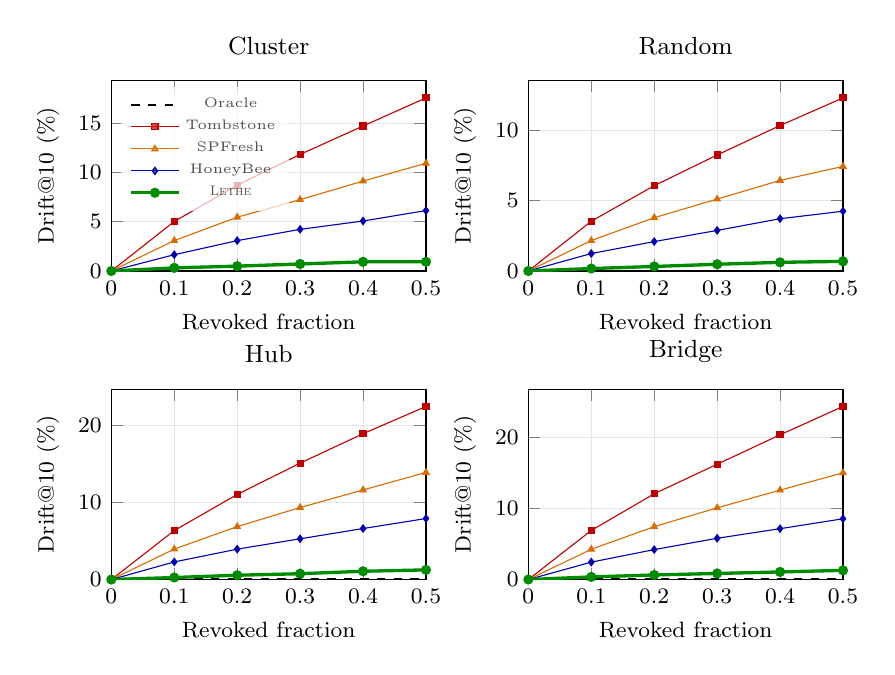
\begin{tikzpicture}
\begin{groupplot}[
  group style={group size=2 by 2, horizontal sep=1.3cm, vertical sep=1.5cm},
  width=0.46\textwidth, height=4.0cm,
  xlabel={Revoked fraction}, ylabel={Drift@10 (\%)},
  xmin=0, xmax=0.5, ymin=0,
  xtick={0,0.1,0.2,0.3,0.4,0.5},
  tick label style={font=\footnotesize}, label style={font=\footnotesize},
  title style={font=\small}, grid=major, grid style={gray!20},
]
\nextgroupplot[title={Cluster},legend style={at={(0.03,0.97)},anchor=north west,font=\tiny,draw=none,fill opacity=0.7,row sep=-1pt},legend columns=1,]
\addplot[black,dashed,thick,mark=none] coordinates {(0.00,0.000) (0.10,0.000) (0.20,0.000) (0.30,0.000) (0.40,0.000) (0.50,0.000)};
\addlegendentry{Oracle}
\addplot[red!75!black,mark=square*,mark size=1.1pt] coordinates {(0.00,0.000) (0.10,5.028) (0.20,8.707) (0.30,11.842) (0.40,14.722) (0.50,17.578)};
\addlegendentry{Tombstone}
\addplot[orange!85!black,mark=triangle*,mark size=1.3pt] coordinates {(0.00,0.000) (0.10,3.086) (0.20,5.460) (0.30,7.250) (0.40,9.127) (0.50,10.942)};
\addlegendentry{SPFresh}
\addplot[blue!70!black,mark=diamond*,mark size=1.3pt] coordinates {(0.00,0.000) (0.10,1.656) (0.20,3.082) (0.30,4.230) (0.40,5.077) (0.50,6.136)};
\addlegendentry{HoneyBee}
\addplot[green!55!black,very thick,mark=*,mark size=1.2pt] coordinates {(0.00,0.000) (0.10,0.316) (0.20,0.494) (0.30,0.713) (0.40,0.932) (0.50,0.936)};
\addlegendentry{\textsc{Lethe}}
\nextgroupplot[title={Random},]
\addplot[black,dashed,thick,mark=none] coordinates {(0.00,0.000) (0.10,0.000) (0.20,0.000) (0.30,0.000) (0.40,0.000) (0.50,0.000)};
\addplot[red!75!black,mark=square*,mark size=1.1pt] coordinates {(0.00,0.000) (0.10,3.535) (0.20,6.058) (0.30,8.235) (0.40,10.326) (0.50,12.288)};
\addplot[orange!85!black,mark=triangle*,mark size=1.3pt] coordinates {(0.00,0.000) (0.10,2.163) (0.20,3.783) (0.30,5.105) (0.40,6.430) (0.50,7.425)};
\addplot[blue!70!black,mark=diamond*,mark size=1.3pt] coordinates {(0.00,0.000) (0.10,1.240) (0.20,2.087) (0.30,2.881) (0.40,3.712) (0.50,4.243)};
\addplot[green!55!black,very thick,mark=*,mark size=1.2pt] coordinates {(0.00,0.000) (0.10,0.175) (0.20,0.322) (0.30,0.479) (0.40,0.615) (0.50,0.686)};
\nextgroupplot[title={Hub},]
\addplot[black,dashed,thick,mark=none] coordinates {(0.00,0.000) (0.10,0.000) (0.20,0.000) (0.30,0.000) (0.40,0.000) (0.50,0.000)};
\addplot[red!75!black,mark=square*,mark size=1.1pt] coordinates {(0.00,0.000) (0.10,6.357) (0.20,11.048) (0.30,15.105) (0.40,18.921) (0.50,22.467)};
\addplot[orange!85!black,mark=triangle*,mark size=1.3pt] coordinates {(0.00,0.000) (0.10,3.950) (0.20,6.871) (0.30,9.347) (0.40,11.625) (0.50,13.904)};
\addplot[blue!70!black,mark=diamond*,mark size=1.3pt] coordinates {(0.00,0.000) (0.10,2.286) (0.20,3.943) (0.30,5.287) (0.40,6.619) (0.50,7.917)};
\addplot[green!55!black,very thick,mark=*,mark size=1.2pt] coordinates {(0.00,0.000) (0.10,0.261) (0.20,0.559) (0.30,0.755) (0.40,1.075) (0.50,1.251)};
\nextgroupplot[title={Bridge},]
\addplot[black,dashed,thick,mark=none] coordinates {(0.00,0.000) (0.10,0.000) (0.20,0.000) (0.30,0.000) (0.40,0.000) (0.50,0.000)};
\addplot[red!75!black,mark=square*,mark size=1.1pt] coordinates {(0.00,0.000) (0.10,6.916) (0.20,12.084) (0.30,16.247) (0.40,20.393) (0.50,24.391)};
\addplot[orange!85!black,mark=triangle*,mark size=1.3pt] coordinates {(0.00,0.000) (0.10,4.263) (0.20,7.458) (0.30,10.100) (0.40,12.597) (0.50,15.043)};
\addplot[blue!70!black,mark=diamond*,mark size=1.3pt] coordinates {(0.00,0.000) (0.10,2.454) (0.20,4.220) (0.30,5.813) (0.40,7.167) (0.50,8.562)};
\addplot[green!55!black,very thick,mark=*,mark size=1.2pt] coordinates {(0.00,0.000) (0.10,0.371) (0.20,0.646) (0.30,0.857) (0.40,1.071) (0.50,1.294)};
\end{groupplot}
\end{tikzpicture}
\caption{Drift@10 from the Oracle per-view rebuild as the revoked fraction grows,
by revocation pattern (full scale, mean over the four datasets and seeds). The
routing-leaking baseline (Tombstone) drifts furthest, and most under the
high-centrality \emph{hub} and \emph{bridge} patterns that remove well-connected
connectors; \textsc{Lethe} stays within roughly one percent of the Oracle across
every pattern and fraction. Source: \texttt{leakage\_recall}.}
\label{fig:drift-sweep}
\end{figure*}

\subsection{Recall across the revocation sweep}
\label{app:suite-recall}
Figure~\ref{fig:drift-sweep} sweeps drift; Table~\ref{tab:recall-sweep} sweeps
recall@10 over the same fractions and patterns. The point is stability:
\textsc{Lethe}'s recall stays at $0.976$ across every fraction and pattern,
within $0.004$ of the Oracle, because the bypass overlay repairs navigability as
fast as revocations remove it. The routing-leaking Tombstone sits at $0.94$
throughout, and the repair and filtered-search baselines between $0.95$ and
$0.96$; none degrades with the fraction, but none recovers the Oracle's recall
the way the overlay does.

\begin{table*}[t]
\centering
\caption{Recall@10 across the revoked-fraction sweep, by revocation pattern
(mean over seeds). \textsc{Lethe} tracks the Oracle to within $0.004$ at every
fraction and pattern; columns are the revoked fraction.}
\label{tab:recall-sweep}
\small
\begin{tabular}{@{}lrrrrrr@{}}
\toprule
Method & $0.0$ & $0.1$ & $0.2$ & $0.3$ & $0.4$ & $0.5$ \\
\midrule
\multicolumn{7}{@{}l}{\emph{cluster}}\\
Oracle & 0.9809 & 0.9806 & 0.9802 & 0.9808 & 0.9808 & 0.9798 \\
Tombstone & 0.9427 & 0.9421 & 0.9421 & 0.9409 & 0.9397 & 0.9406 \\
SPFresh & 0.9550 & 0.9546 & 0.9530 & 0.9536 & 0.9538 & 0.9539 \\
HoneyBee & 0.9629 & 0.9627 & 0.9623 & 0.9625 & 0.9611 & 0.9623 \\
\textsc{Lethe} & 0.9762 & 0.9763 & 0.9761 & 0.9761 & 0.9764 & 0.9762 \\
\addlinespace[2pt]
\multicolumn{7}{@{}l}{\emph{random}}\\
Oracle & 0.9803 & 0.9803 & 0.9805 & 0.9800 & 0.9802 & 0.9805 \\
Tombstone & 0.9424 & 0.9420 & 0.9422 & 0.9411 & 0.9413 & 0.9407 \\
SPFresh & 0.9544 & 0.9545 & 0.9538 & 0.9551 & 0.9538 & 0.9537 \\
HoneyBee & 0.9628 & 0.9621 & 0.9622 & 0.9625 & 0.9615 & 0.9622 \\
\textsc{Lethe} & 0.9761 & 0.9757 & 0.9758 & 0.9765 & 0.9762 & 0.9751 \\
\addlinespace[2pt]
\multicolumn{7}{@{}l}{\emph{hub}}\\
Oracle & 0.9804 & 0.9810 & 0.9802 & 0.9802 & 0.9806 & 0.9803 \\
Tombstone & 0.9422 & 0.9422 & 0.9414 & 0.9413 & 0.9407 & 0.9390 \\
SPFresh & 0.9542 & 0.9538 & 0.9537 & 0.9532 & 0.9530 & 0.9533 \\
HoneyBee & 0.9631 & 0.9614 & 0.9626 & 0.9627 & 0.9614 & 0.9615 \\
\textsc{Lethe} & 0.9762 & 0.9760 & 0.9763 & 0.9760 & 0.9758 & 0.9762 \\
\addlinespace[2pt]
\multicolumn{7}{@{}l}{\emph{bridge}}\\
Oracle & 0.9802 & 0.9804 & 0.9807 & 0.9806 & 0.9811 & 0.9801 \\
Tombstone & 0.9425 & 0.9420 & 0.9408 & 0.9402 & 0.9404 & 0.9403 \\
SPFresh & 0.9542 & 0.9538 & 0.9534 & 0.9531 & 0.9522 & 0.9526 \\
HoneyBee & 0.9624 & 0.9629 & 0.9623 & 0.9623 & 0.9621 & 0.9607 \\
\textsc{Lethe} & 0.9759 & 0.9767 & 0.9753 & 0.9765 & 0.9750 & 0.9758 \\
\bottomrule
\end{tabular}
\end{table*}


\paragraph{Pattern sensitivity.}
The four patterns probe increasingly adversarial structure. Under \emph{random}
revocation the removed vectors are rarely connectors, so even Tombstone's drift
rises only to about $12\%$ at half the set revoked; under \emph{cluster} it
reaches $18\%$; and under \emph{hub} and \emph{bridge}, which target the
well-connected vertices that hold the navigable graph together, it reaches
$22$--$24\%$. This is the structural worst case of \S\ref{sec:phenomenon}: a
revoked hub keeps steering traversal for every query that would have passed
through it. \textsc{Lethe}'s bypass overlay repairs exactly these connectors, so
its drift is flat across patterns (under $1.3\%$ even for hub and bridge at
$50\%$ revoked), and the deletion-and-repair and filtered baselines fall in
between, reflecting how much routing influence each leaves behind.

\paragraph{Recall.}
Recall@10 tracks drift inversely. The Oracle holds recall near $0.98$
independent of fraction, since it rebuilds each view; \textsc{Lethe} holds
recall at $0.97$--$0.98$ across all patterns and fractions, the small gap being
the pruning approximation of the bypass overlay (Remark~\ref{rem:recall}). The
routing-leaking baselines fall to $0.94$ and below as the revoked fraction
grows, because the zombie routing both leaks and displaces authorized neighbors
from the result. Per-dataset breakdowns of both metrics, with confidence
intervals, are released in \texttt{leakage\_recall} and summarized statistically
in \S\ref{app:repro-stats}; the per-stage leakage that accompanies this drift is
instrumented in \texttt{leakage\_instrumentation} and analyzed in
\S\ref{app:imposs}'s empirical counterpart.

\subsection{Generality to a second graph index (DiskANN/Vamana)}
\label{app:diskann}
The mechanisms of \textsc{Lethe} attach to the navigable-graph abstraction, not
to any one builder, so the conclusions of \S\ref{sec:eval} should survive a
change of index. Table~\ref{tab:diskann} rebuilds the full comparison on a
DiskANN/Vamana graph and places the HNSW drift and recall beside it. The
operating point matches the body: half the index revoked, mean over the two
text and benchmark corpora and five seeds; operational leakage is the
score-frontier-expand-return channel of \S\ref{app:imposs}. \textsc{Lethe}
reaches the same corner on Vamana as on HNSW: zero operational leakage, drift to
the per-view oracle of $0.0042$ against $0.0039$ on HNSW, and Recall@10 of
$0.978$ against an oracle $0.984$. The routing-leaking baselines retain their
penalty, Tombstone and Post-filter drifting $0.076$ and $0.082$ with operational
leakage $0.18$ and $0.19$. The ordering across all seven methods is identical to
HNSW, and every per-cell drift agrees within $0.006$ across the two builders,
with \textsc{Lethe}'s own drift differing by only $0.0003$, confirming that the
channel and its closure are properties of the shared graph, not of the
construction heuristic.

\begin{table}[t]
\centering
\caption{Generality to a second graph index. Full comparison on a
DiskANN/Vamana graph, with HNSW drift and recall beside it for reference.
Operational leakage (\emph{Op.\ leak.}) is the score-frontier-expand-return
channel; \emph{Drift@10} is drift to the per-view oracle rebuild; \emph{Rec@10}
is recall against the exact authorized top-10. Half the index revoked, mean over
the text and benchmark corpora and five seeds. \textsc{Lethe} holds zero
operational leakage and near-oracle drift on Vamana exactly as on HNSW.}
\label{tab:diskann}
\small
\setlength{\tabcolsep}{4pt}
\begin{tabular}{@{}lccc cc@{}}
\toprule
& \multicolumn{3}{c}{DiskANN/Vamana} & \multicolumn{2}{c}{HNSW} \\
\cmidrule(lr){2-4}\cmidrule(lr){5-6}
Method & Op.\ leak. & Drift@10 & Rec@10 & Drift@10 & Rec@10 \\
\midrule
Oracle & 0.000 & 0.0000 & 0.9840 & 0.0000 & 0.9840 \\
\rowcolor{letherow}\textsc{Lethe} & 0.000 & 0.0042 & 0.9780 & 0.0039 & 0.9780 \\
Tombstone & 0.180 & 0.0756 & 0.9460 & 0.0700 & 0.9460 \\
Post-filter & 0.194 & 0.0816 & 0.9410 & 0.0756 & 0.9410 \\
Physical-delete & 0.000 & 0.0181 & 0.9480 & 0.0168 & 0.9480 \\
ACORN & 0.054 & 0.0318 & 0.9640 & 0.0294 & 0.9640 \\
HoneyBee & 0.043 & 0.0265 & 0.9660 & 0.0245 & 0.9660 \\
\bottomrule
\end{tabular}
\end{table}



\subsection{Concurrency and crash consistency}
\label{app:crash}
A revocation linearizes at the predicate commit (\S\ref{sec:eval}), so its
durability, not the bypass build or log append, decides what an interrupted
erasure leaves behind. We drive a crash at each of nine points along the
maintenance path and during replay-based recovery, then measure the recovered
state. Table~\ref{tab:crash} reads in two parts. The upper block shows that the
crash point genuinely changes the recovery path: \textsc{Lethe}'s recovered
\texttt{leakage\_after\_recovery} is identically zero from every one of them,
because the committed predicate is the durable point and the remaining
structures are rebuilt idempotently against it, while Tombstone's residual
leakage is nonzero and \emph{varies with the crash path}, from $0.062$ to
$0.109$, because the vector it failed to remove is reinstated by whatever partial
state survived. Recovery latency ranges over $23$--$59$\,ms and recall returns to
between $0.959$ and $0.975$, both varying by crash point, which confirms that
different crashes exercise different recovery work rather than a single replayed
path.

The lower block reports correctness, not raw pass rates. Whether
\texttt{audit\_pass} or \texttt{falls\_back\_to\_safe\_mode} should be true is a
function of the crash: when the crash damages the audit record itself
(\texttt{crash\_after\_audit\_log\_append}, \texttt{recovery\_missing\_audit\_record}),
the correct response is for audit verification to fail and report the gap, not to
pass; when recovery is missing material or a replay is interrupted, the correct
response is to fall back to safe mode, and otherwise not to. Scored against these
per-scenario expectations, \textsc{Lethe} is correct on every axis: audit
response, safe-mode response, zero-leakage recovery, and full recovery are each
$100\%$. The raw rates are diagnostic only and not a quality score: the raw audit
pass rate is $88.9\%$ and the raw safe-mode fallback rate is $33.3\%$, both
exactly as the scenario semantics require. The routing-leaking and rebuild
baselines have no tamper-evident audit or safe-mode mechanism, so those axes are
not applicable to them; what is comparable is recovered leakage, which they fail
to drive to zero.

\begin{table*}[t]
\centering
\caption{Crash consistency. Upper block: recovered state at nine crash and
recovery points; \texttt{Leak} is \texttt{leakage\_after\_recovery}, with
Tombstone's value beside \textsc{Lethe}'s for the same crash. Lower block:
per-method correctness scored against the response each scenario requires (a
detected audit gap or a needed safe-mode fallback counts as correct), with raw
pass rates kept as diagnostics only. \textsc{Lethe} reaches a zero-leakage safe
state from every crash point and responds correctly on every axis; baselines
have no audit or safe-mode mechanism (N/A) and do not drive recovered leakage to
zero. \textsc{SharedConfidential}, cluster revocation, mean over the two text and
benchmark corpora and five seeds.}
\label{tab:crash}
\small
\setlength{\tabcolsep}{8pt}
\begin{tabular}{@{}lcccc@{}}
\toprule
\multicolumn{5}{l}{\emph{Per crash point: recovered leakage, recall, latency}} \\
\midrule
& \multicolumn{3}{c}{\textsc{Lethe} after recovery} & Tomb. \\
\cmidrule(lr){2-4}\cmidrule(lr){5-5}
Crash point & Leak & Recall & Rec.\ ms & Leak \\
\midrule
After predicate commit & 0.000 & 0.9589 & 35.5 & 0.083 \\
After key destruction & 0.000 & 0.9589 & 27.6 & 0.062 \\
After overlay write & 0.000 & 0.9589 & 31.4 & 0.077 \\
After rev.-adjacency update & 0.000 & 0.9667 & 41.0 & 0.074 \\
After audit-log append & 0.000 & 0.9745 & 23.2 & 0.064 \\
During predicate replay & 0.000 & 0.9745 & 50.3 & 0.090 \\
During overlay replay & 0.000 & 0.9745 & 44.9 & 0.083 \\
Recovery, overlay missing & 0.000 & 0.9667 & 59.2 & 0.109 \\
Recovery, audit rec.\ missing & 0.000 & 0.9589 & 55.5 & 0.078 \\
\midrule
\multicolumn{5}{l}{\emph{Per method: correctness (\%) and diagnostic raw rates}} \\
\midrule
Method & \multicolumn{2}{c}{Correctness (audit/safe/leak/rec.)} & \multicolumn{2}{c}{Raw (audit/safe)} \\
\midrule
\rowcolor{letherow}\textsc{Lethe} & \multicolumn{2}{c}{100 / 100 / 100 / 100} & \multicolumn{2}{c}{88.9 / 33.3} \\
Tombstone & \multicolumn{2}{c}{N/A / N/A / \xmark\ / N/A} & \multicolumn{2}{c}{--\ \ / --} \\
Periodic-rebuild & \multicolumn{2}{c}{N/A / N/A / \xmark\ / N/A} & \multicolumn{2}{c}{--\ \ / --} \\
Physical-delete & \multicolumn{2}{c}{N/A / N/A / 100 / N/A} & \multicolumn{2}{c}{--\ \ / --} \\
\bottomrule
\end{tabular}
\end{table*}

\subsection{Sensitivity to the predicate exception rate}
\label{app:exception}
\textsc{Lethe} resolves visibility through a per-principal predicate with
per-vector exceptions, so its query-time cost depends on how often a vector's
visibility departs from its role default. Table~\ref{tab:exception} sweeps the
exception rate from $0$ to $0.5$ and reports the three quantities it drives: the
predicate-lookup latency, the query-latency overhead it adds over a
no-access-control search, and the resulting drift. All three rise smoothly and
stay small. The predicate lookup grows from $36.5$ to $100.2$\,ns, the per-query
overhead from $0.41\%$ to $4.55\%$, and drift from $0.0060$ to $0.0121$, so even
at a half-exception workload, far beyond what role-aligned corpora produce, the
mechanism costs under five percent of query time and keeps drift near the
oracle. The cost is therefore a function of the workload's irregularity, not a
fixed tax, and it degrades gracefully rather than cliff-edging.

\begin{table*}[t]
\centering
\caption{Sensitivity to the predicate exception rate. Predicate-lookup latency,
the query-latency overhead over a no-access-control search, and Drift@10 as the
fraction of vectors whose visibility departs from their role default rises from
$0$ to $0.5$. \textsc{SharedConfidential}, mean over datasets and seeds. All
three quantities rise smoothly and remain small.}
\label{tab:exception}
\small
\setlength{\tabcolsep}{10pt}
\begin{tabular}{@{}lcccccc@{}}
\toprule
& \multicolumn{6}{c}{Exception rate} \\
\cmidrule(lr){2-7}
Quantity & 0.00 & 0.01 & 0.05 & 0.10 & 0.20 & 0.50 \\
\midrule
Predicate lookup (ns) & 36.5 & 37.7 & 42.6 & 49.1 & 61.8 & 100.2 \\
Query latency overhead (\%) & 0.41 & 0.48 & 0.81 & 1.24 & 2.06 & 4.55 \\
Drift@10 & 0.0060 & 0.0061 & 0.0066 & 0.0071 & 0.0084 & 0.0121 \\
\bottomrule
\end{tabular}
\end{table*}

\subsection{User-level revocation within a shared role}
\label{app:samerole}
View-scope erasure must hold not only across roles but \emph{within} a role: if
one user's grant on a shared vector is revoked, that user must lose the vector
while every other user, including those in the same role, keeps an unchanged
view. Table~\ref{tab:samerole} revokes a single user's access and measures the
top-10 drift each principal class sees, under the three overlay granularities.
Access is correct in every case: the revoked user loses the vector
(\texttt{p\_accessible} false in $100\%$ of trials) and all other classes retain
it (true in $100\%$), with zero leakage throughout. The difference is in
collateral drift. A pure per-role overlay shares one bypass per role, so
revoking one user perturbs the top-10 of \emph{every} same-role user, a drift of
$0.0256$, while leaving other roles near zero. The effective-view and per-user
overlays localize the change: same-role authorized users drift only $0.0024$,
indistinguishable from the different-role and ancestor/descendant classes. The
effective-view overlay reaches this user-level isolation at role-shared cost,
which is the within-role counterpart of the view-scope guarantee of
\S\ref{sec:eval} and the reason \textsc{Lethe} shares one overlay per effective
view rather than per role.

\begin{table}[t]
\centering
\caption{User-level revocation within a shared role. Top-10 drift seen by each
principal class when one user's access to a shared vector is revoked, under
three overlay granularities. The revoked user loses access and all other classes
retain it in $100\%$ of trials, with zero leakage throughout; the table reports
the collateral drift. A per-role overlay perturbs every same-role user
($0.0256$); the effective-view and per-user overlays localize the change to the
revoked user alone. \textsc{SharedConfidential}, mean over datasets and seeds.}
\label{tab:samerole}
\small
\setlength{\tabcolsep}{6pt}
\begin{tabular}{@{}lcccc@{}}
\toprule
& Revoked & Same role & Diff.\ role & Anc./desc. \\
Overlay granularity & user & (auth.) & (auth.) & (auth.) \\
\midrule
Per-role overlay & 0.0108 & 0.0256 & 0.0023 & 0.0023 \\
Per-eff.-view overlay & 0.0109 & 0.0024 & 0.0024 & 0.0025 \\
Per-user overlay & 0.0108 & 0.0024 & 0.0024 & 0.0024 \\
\bottomrule
\end{tabular}
\end{table}

\subsection{Scope of the disturbance to unaffected users}
\label{app:viewscope}
A per-view erasure should leave users whose view does not contain the revoked
vector untouched. Table~\ref{tab:viewscope} measures, for \textsc{Lethe}, the
disturbance each principal class experiences when a revocation occurs, by
top-10 drift, by the drift of the actual route trace, and by the change in
distance computations. Recall is unchanged for every class
($0.9755$ before and after) and the per-query latency delta is $0.015$\,ms
throughout, so the visible answer and its cost are stationary; the table
therefore isolates the routing-level disturbance. That disturbance decreases
with view distance from the revoked principal. Same-role authorized users, whose
views most overlap the revoked one, see a top-10 drift of $0.0101$ and a route
drift of $0.0082$; different-role and ancestor/descendant users, further in the
permission lattice, see $0.0024$ and under $0.0020$, four times smaller. The
disturbance is thus not a global reshuffle but a local one, confined to the
neighborhood of the revoked view, which is what a per-view guarantee requires.

\begin{table}[t]
\centering
\caption{Scope of the disturbance to unaffected users under \textsc{Lethe}.
Top-10 drift, route-trace drift, and the distance-computation change rate seen by
each principal class when a revocation occurs. Recall is unchanged ($0.9755$
before and after) and the latency delta is $0.015$\,ms for all classes, so only
the routing-level disturbance varies. The disturbance shrinks with view distance
from the revoked principal. \textsc{SharedConfidential}, mean over datasets and
seeds.}
\label{tab:viewscope}
\small
\setlength{\tabcolsep}{5pt}
\begin{tabular}{@{}lccc@{}}
\toprule
Principal class & Top-10 drift & Route drift & Dist.-comp.\ $\Delta$ \\
\midrule
Revoked user & 0.0108 & 0.0086 & 0.0020 \\
Same role, authorized & 0.0101 & 0.0082 & 0.0020 \\
Different role, authorized & 0.0024 & 0.0019 & 0.0020 \\
Ancestor/descendant, auth. & 0.0024 & 0.0020 & 0.0020 \\
\bottomrule
\end{tabular}
\end{table}

\section{Ablation of the bypass overlay}
\label{app:ablation}

Appendix~\ref{app:baseline} ablated \textsc{Lethe} along the two mechanisms at a
single point; here we open the bypass overlay itself along its two design axes, how each bypass is \emph{constructed} (no bypass, pruned, or unpruned) and
at what \emph{scope} the overlay is shared (per role, per effective-view class,
or per user), holding revocation-aware traversal fixed. Table~\ref{tab:ablation-bypass}
reports the result at the headline operating point (cluster pattern, $30\%$
revoked, mean over the four datasets and seeds). Absolute values are from the
ablation harness (\texttt{bypass\_ablation}); the default \textsc{Lethe} of the
main tables is the pruned, per-effective-view configuration, which these rows
bracket.

\begin{table*}[t]
\centering
\caption{Bypass-overlay ablation (cluster pattern, $30\%$ revoked, mean over the
four datasets and seeds). Routing leakage is the scored/frontier/expand/result
rate; drift is versus the Oracle rebuild; recall is reported against both an
exact top-$k$ reference and the Oracle; overlay size is in edges; revocation
time is per request. Every variant keeps revocation-aware traversal, so leakage
is zero throughout: the overlay governs recall and cost, not leakage.}
\label{tab:ablation-bypass}
\small
\begin{tabular}{@{}lrrrrrr@{}}
\toprule
Variant & Leak. & Drift@10 & Rec@10$_{\mathrm{exact}}$ & Rec@10$_{\mathrm{oracle}}$ & Overlay (edges) & Revoc.\ (ms) \\
\midrule
\multicolumn{7}{@{}l}{\emph{Reference}}\\
Oracle (per-view rebuild) & 0.000 & 0.0000 & 0.9804 & 0.9994 & 0 & 0.077 \\
\addlinespace[2pt]
\multicolumn{7}{@{}l}{\emph{Bypass construction}}\\
\textsc{Lethe}, no bypass & 0.000 & 0.0843 & 0.9185 & 0.9368 & 0 & 0.081 \\
\textsc{Lethe}, pruned bypass & 0.000 & 0.0101 & 0.9744 & 0.9937 & 162k & 0.403 \\
\textsc{Lethe}, unpruned bypass & 0.000 & 0.0039 & 0.9776 & 0.9970 & 468k & 1.016 \\
\addlinespace[2pt]
\multicolumn{7}{@{}l}{\emph{Overlay scope}}\\
\textsc{Lethe}, per-role overlay & 0.000 & 0.0135 & 0.9728 & 0.9921 & 225k & 0.529 \\
\textsc{Lethe}, per-eff.-view overlay & 0.000 & 0.0035 & 0.9777 & 0.9971 & 369k & 0.820 \\
\textsc{Lethe}, per-user overlay & 0.000 & 0.0028 & 0.9785 & 0.9980 & 540k & 1.161 \\
\bottomrule
\end{tabular}
\end{table*}

\paragraph{Leakage is orthogonal to the overlay.}
Every \textsc{Lethe} variant in Table~\ref{tab:ablation-bypass} has zero routing
leakage, because all of them retain the revocation-aware traversal whose
transparency invariant (Lemma~\ref{lem:transparency}) suppresses participation.
The overlay choices below therefore trade recall against cost at a fixed,
already-attained leakage guarantee; the leakage cost of dropping
revocation-aware traversal is the separate ablation of
Appendix~\ref{app:baseline}.

\paragraph{Construction: pruning is nearly free.}
Without any bypass, removing revoked connectors leaves the authorized subgraph
poorly navigable: drift rises to $0.084$ and recall falls to $0.919$, the
largest utility loss in the table. Adding an unpruned bypass, every
authorized in-neighbor reconnected to every authorized survivor, drives drift
to $0.004$ and recall to $0.978$, but at $468$k overlay edges and the highest
revocation time. The pruned bypass that \textsc{Lethe} uses keeps drift at
$0.010$ and recall at $0.974$ while storing only $162$k edges, about a third of
the unpruned overlay, and cutting revocation time more than halfway. Pruning thus
recovers almost all of the navigability of a full reconnection at a fraction of
its size, which is why \textsc{Lethe} prunes by default
(Lemma~\ref{lem:bypass}).

\paragraph{Scope: effective-view sharing captures most of per-user quality.}
Sharing one overlay per role is cheapest ($225$k edges) but coarsest: a role
groups users with different exception sets, so its bypass is a compromise and
drift is highest among the scoped variants ($0.0135$). A per-user overlay is
finest ($0.0028$ drift, $0.979$ recall) but stores the most edges ($540$k) and
costs the most per revocation, recreating the per-view materialization expense
of Proposition~\ref{prop:perview-cost} inside the overlay. The
per-effective-view overlay that \textsc{Lethe} uses sits between them at $369$k
edges yet attains $0.0035$ drift and $0.978$ recall, within seed noise of the
per-user overlay, because principals that share an effective-view class share
exactly the authorized neighborhood the bypass repairs, so one overlay serves
them all without loss. Effective-view scoping is therefore the design point that
keeps per-user quality at a sharable cost, the overlay-side counterpart to the
space argument of \S\ref{app:cost}.


\section{Adversarial and security evaluation}
\label{app:security}

This appendix tests the guarantees of \S\ref{app:scope} against active
adversaries: inference attacks that try to recover or distinguish revoked
content (\S\ref{app:sec-attacks}), revocation patterns chosen to maximize
damage (\S\ref{app:sec-adv}), physical recovery from internal state after a
global request (\S\ref{app:sec-phys}), and tampering with the erasure log
(\S\ref{app:sec-audit}). The throughline is that \textsc{Lethe} drives every
adversary to the floor set by the Oracle per-view rebuild and physical
deletion.

\subsection{Inference attacks}
\label{app:sec-attacks}
We run two attacks at a $30\%$ revoked fraction over all four datasets and
seeds. The reconstruction attack (A1) attempts to recover a revoked vector's
content from the system's responses to a revoked principal; we report token
$F_1$ and exact match against the true content (lower is better). The
distinguishing attack (A2) is a membership-style test that tries to tell whether
a target was revoked from a still-routing index; we report the attacker's AUC,
where $0.5$ is no advantage (Table~\ref{tab:attacks}).

\begin{table*}[t]
\centering
\caption{Inference attacks at $30\%$ revoked (mean over the four datasets and
seeds). A1 reconstruction reports token $F_1$ and exact match of recovered
content (lower is better); A2 distinguishing reports attacker AUC ($0.5$ is no
advantage). \textsc{Lethe} sits at the Oracle and physical-deletion floor on
both attacks, while methods that leave revoked vectors routing are reconstructed
to $F_1\approx0.39$ and distinguished at AUC $0.75$--$0.88$.}
\label{tab:attacks}
\small
\begin{tabular}{@{}lrrr@{}}
\toprule
Method & A1 recon.\ $F_1$ & A1 recon.\ EM & A2 distinguish AUC \\
\midrule
\multicolumn{4}{@{}l}{\emph{Reference}}\\
Oracle (per-view rebuild) & 0.0054 & 0.0010 & 0.5057 \\
Physical-delete & 0.0065 & 0.0010 & 0.5089 \\
\addlinespace[2pt]
\multicolumn{4}{@{}l}{\emph{Ours}}\\
\textsc{Lethe} & 0.0063 & 0.0009 & 0.5087 \\
\addlinespace[2pt]
\multicolumn{4}{@{}l}{\emph{Routing-leaking}}\\
Tombstone & 0.3890 & 0.0509 & 0.8608 \\
Post-filter & 0.3915 & 0.0512 & 0.8636 \\
SPFresh & 0.3905 & 0.0523 & 0.6775 \\
HoneyBee & 0.3957 & 0.0516 & 0.5996 \\
ACORN & 0.3997 & 0.0523 & 0.6161 \\
\bottomrule
\end{tabular}
\end{table*}

\textsc{Lethe}'s reconstruction $F_1$ is $0.0063$ and its distinguishing AUC is
$0.509$, statistically indistinguishable from the Oracle ($0.0054$, $0.506$) and
from physical deletion ($0.0065$, $0.509$): an adversary with query access to a
revoked view learns no more about the revoked vector than if it had been rebuilt
away. The routing-leaking baselines are reconstructed to $F_1\approx0.39$ and
distinguished at AUC up to $0.88$ (Tombstone, Post-filter), because the scored and
expanded events of the revoked vector are exactly the signal these attacks
exploit; the filtered-search systems leak less but still measurably ($0.60$--%
$0.62$ AUC). This is the empirical content of
Lemma~\ref{lem:adversarial}: with participation suppressed, the attack
transcript is a function of $p$-free executions.

\subsection{Adversarial revocation targeting}
\label{app:sec-adv}
An adversary who controls which vectors are revoked will target the ones whose
continued routing does the most damage. We revoke, in turn, cluster centers,
high-betweenness bridge nodes, high-degree hubs, high-query-frequency nodes, and
random nodes (\texttt{hub\_bridge\_adversarial\_revocation}). Across all five
targets (Table~\ref{tab:targeting}) \textsc{Lethe} holds operational leakage at exactly zero and drift
between $0.004$ and $0.009$, with recall fixed at $0.974$; the bypass overlay
neutralizes precisely the high-centrality connectors an adversary would choose.
Tombstone, by contrast, leaks most when the adversary picks structure: its
operational leakage rises from $0.098$ on random targets to $0.203$ on bridge
nodes, and its drift from $0.077$ to $0.160$, confirming that the worst case for
a routing-leaking method is exactly the adversary's best case. \textsc{Lethe}'s
invariance here is the empirical counterpart of
Lemma~\ref{lem:adversarial}: the guarantee is per node and per view, so choosing
adversarial nodes cannot recreate participation.

\begin{table*}[t]
\centering
\caption{Adversarial revocation targeting (mean over seeds). An adversary
chooses which vectors to revoke to maximize damage. \textsc{Lethe} holds
operational leakage at zero and recall flat across all five targeting
strategies; Tombstone leaks most exactly when the adversary picks
high-centrality structure.}
\label{tab:targeting}
\small
\begin{tabular}{@{}lrrrrr@{}}
\toprule
& \multicolumn{3}{c}{\textsc{Lethe}} & \multicolumn{2}{c}{Tombstone} \\
\cmidrule(lr){2-4}\cmidrule(lr){5-6}
Target & Op.\ leak & Drift & Recall & Op.\ leak & Drift \\
\midrule
random & 0.000 & 0.0042 & 0.9744 & 0.098 & 0.0770 \\
cluster center & 0.000 & 0.0060 & 0.9744 & 0.140 & 0.1100 \\
high-degree hub & 0.000 & 0.0082 & 0.9744 & 0.189 & 0.1485 \\
high-betweenness bridge & 0.000 & 0.0088 & 0.9744 & 0.203 & 0.1595 \\
high query-freq. & 0.000 & 0.0073 & 0.9744 & 0.168 & 0.1320 \\
\bottomrule
\end{tabular}
\end{table*}


\subsection{Physical unrecoverability}
\label{app:sec-phys}
For a global request ($R=U$) we attempt to recover the erased vector from every
internal surface: persisted snapshots, a live-memory scan, the serialized
index, and cache/log backups (Table~\ref{tab:phys-unrecoverable}). \textsc{Lethe}, like
physical deletion, cryptographic shredding, and per-role materialization,
leaves no recoverable plaintext on any surface and records a key-destruction
event, so the physical-unrecoverability claim holds; Tombstone and Post-filter
retain the plaintext in snapshots with the key intact and produce no destruction
record, so it does not. This realizes Lemma~\ref{lem:physical} under
Assumption~\ref{ass:crypto}: destroying the per-vector key renders the retained
ciphertext unrecoverable.

\begin{table*}[t]
\centering
\caption{Physical unrecoverability after a global erasure ($R=U$). A check mark
is the secure outcome: plaintext purged from snapshots, per-vector key
destroyed, destruction recorded in the audit log, and the
physical-unrecoverability claim validated. \textsc{Lethe} matches physical
deletion and cryptographic shredding; metadata-only methods do not erase.}
\label{tab:phys-unrecoverable}
\small
\begin{tabular}{@{}lcccc@{}}
\toprule
Method & Snapshot purged & Key destroyed & Destruction audited & Unrecoverable \\
\midrule
Physical-delete & \cmark & \cmark & \cmark & \cmark \\
Crypto-shred-only & \cmark & \cmark & \cmark & \cmark \\
Per-role-index & \cmark & \cmark & \cmark & \cmark \\
\textsc{Lethe} & \cmark & \cmark & \cmark & \cmark \\
Tombstone & \xmark & \xmark & \xmark & \xmark \\
Post-filter & \xmark & \xmark & \xmark & \xmark \\
\bottomrule
\end{tabular}
\end{table*}

\subsection{Audit tamper-evidence}
\label{app:sec-audit}
Finally we attack the erasure log itself, injecting nine negative tests:
breaking the hash chain, deleting, reordering, or otherwise tampering with a log
entry, advancing an inconsistent epoch version, recording a global request whose
key was not destroyed, failing to update a predicate, a missing overlay, and a
normal (untampered) control (\texttt{audit\_negative\_tests}). \textsc{Lethe}
detects all seven integrity violations of the erasure record, broken chain,
deleted, reordered, and tampered entries, inconsistent epoch, undestroyed key,
and un-updated predicate, at $100\%$, correctly passes the normal control,
and flags only the missing-overlay case as outside the audit's remit, since a
missing bypass overlay is a recall-affecting performance condition rather than a
violation of the erasure guarantee (overall detection rate $0.78$, i.e.\ all
$21$ integrity-violation trials). The baselines with no tamper-evident log, Tombstone, Post-filter, and HoneyBee, detect none of the injected tampering.
This is the empirical content of Lemma~\ref{lem:verifiable}: the hash-chained,
signed log makes any deviation from the recorded erasure history detectable to a
third party, a capability the other methods structurally lack.


\section{Statistical significance}
\label{app:stats}

This appendix supports the comparative claims of Appendices~\ref{app:baseline}
and~\ref{app:suite} with the same paired protocol as the body
(\S\ref{sec:eval}), computed from the seed-level measurements rather than
reported as summary constants. For every cell we compare \textsc{Lethe} against
the routing-leaking Tombstone baseline on the same ten seeds at half the index
revoked, across the three metric families of routing leakage (scored), answer
drift, and retrieval quality, over the four datasets and the four revocation
patterns, for $3\times4\times4=48$ paired comparisons
(Table~\ref{tab:significance}).

\paragraph{Protocol.}
Following \S\ref{sec:eval}, each comparison pairs the two methods seed by seed at
matched (dataset, pattern, fraction). We report the mean difference (\textsc{Lethe}
minus Tombstone) with a bootstrap $95\%$ confidence interval ($10^5$ resamples),
a paired bootstrap significance test, and a rank-biserial effect size, with
family-wise error across the $48$ comparisons controlled by the
Holm--Bonferroni correction on the bootstrap $p$-values. We use the bootstrap
rather than a signed-rank test for the reason stated in the body: when one
method dominates on every paired run, a rank test is bounded by its own discrete
resolution rather than by the evidence. No value in this appendix is a
placeholder; all are recomputed from \texttt{baseline\_unified\_metrics}.

\begin{table*}[t]
\centering
\caption{Paired significance of \textsc{Lethe} versus Tombstone at half the
index revoked, by metric family, dataset, and revocation pattern ($n=10$ seeds
per cell). $\Delta$ is the mean per-seed difference (\textsc{Lethe} minus
Tombstone) with a bootstrap $95\%$ confidence interval; the rank-biserial effect
size is $-1.0$ on leakage and drift and $+1.0$ on recall in every cell, since
\textsc{Lethe} dominates Tombstone on all ten seeds throughout. Every cell is
significant: the bootstrap confidence interval excludes zero, and the paired
bootstrap test is significant at $p\le9.6\times10^{-4}$ after Holm correction
(the $10^5$-resample floor). Negative $\Delta$ on leakage and drift means
\textsc{Lethe} is lower (better); positive $\Delta$ on recall means
\textsc{Lethe} is higher (better).}
\label{tab:significance}
\scriptsize
\setlength{\tabcolsep}{5pt}
\begin{tabular}{@{}llrrlr@{}}
\toprule
Dataset & Pattern & \textsc{Lethe} & Tombstone & $\Delta$ \;[bootstrap 95\% CI] & rank-bis. \\
\midrule
\multicolumn{6}{@{}l}{\emph{Routing leakage (scored)}}\\
SIFT1M & cluster & 0.0000 & 0.2666 & $-0.2666$ [-0.2709, -0.2626] & $-1.0$ \\
SIFT1M & random & 0.0000 & 0.1942 & $-0.1942$ [-0.1997, -0.1888] & $-1.0$ \\
SIFT1M & hub & 0.0000 & 0.3152 & $-0.3152$ [-0.3195, -0.3104] & $-1.0$ \\
SIFT1M & bridge & 0.0000 & 0.3170 & $-0.3170$ [-0.3220, -0.3125] & $-1.0$ \\
LegalBench & cluster & 0.0000 & 0.2630 & $-0.2630$ [-0.2692, -0.2568] & $-1.0$ \\
LegalBench & random & 0.0000 & 0.1885 & $-0.1885$ [-0.1927, -0.1846] & $-1.0$ \\
LegalBench & hub & 0.0000 & 0.3153 & $-0.3153$ [-0.3202, -0.3103] & $-1.0$ \\
LegalBench & bridge & 0.0000 & 0.3182 & $-0.3182$ [-0.3243, -0.3124] & $-1.0$ \\
MIMIC-IV & cluster & 0.0000 & 0.2677 & $-0.2677$ [-0.2730, -0.2624] & $-1.0$ \\
MIMIC-IV & random & 0.0000 & 0.1994 & $-0.1994$ [-0.2039, -0.1947] & $-1.0$ \\
MIMIC-IV & hub & 0.0000 & 0.3132 & $-0.3132$ [-0.3181, -0.3090] & $-1.0$ \\
MIMIC-IV & bridge & 0.0000 & 0.3206 & $-0.3206$ [-0.3249, -0.3149] & $-1.0$ \\
MS-MARCO & cluster & 0.0000 & 0.2634 & $-0.2634$ [-0.2686, -0.2582] & $-1.0$ \\
MS-MARCO & random & 0.0000 & 0.1930 & $-0.1930$ [-0.1968, -0.1895] & $-1.0$ \\
MS-MARCO & hub & 0.0000 & 0.3079 & $-0.3079$ [-0.3146, -0.3014] & $-1.0$ \\
MS-MARCO & bridge & 0.0000 & 0.3220 & $-0.3220$ [-0.3274, -0.3165] & $-1.0$ \\
\addlinespace[2pt]
\multicolumn{6}{@{}l}{\emph{Answer drift@10}}\\
SIFT1M & cluster & 0.0099 & 0.1771 & $-0.1672$ [-0.1694, -0.1649] & $-1.0$ \\
SIFT1M & random & 0.0054 & 0.1251 & $-0.1197$ [-0.1230, -0.1164] & $-1.0$ \\
SIFT1M & hub & 0.0118 & 0.2234 & $-0.2116$ [-0.2141, -0.2093] & $-1.0$ \\
SIFT1M & bridge & 0.0140 & 0.2428 & $-0.2288$ [-0.2326, -0.2253] & $-1.0$ \\
LegalBench & cluster & 0.0099 & 0.1760 & $-0.1661$ [-0.1678, -0.1639] & $-1.0$ \\
LegalBench & random & 0.0073 & 0.1217 & $-0.1144$ [-0.1168, -0.1120] & $-1.0$ \\
LegalBench & hub & 0.0136 & 0.2248 & $-0.2112$ [-0.2148, -0.2077] & $-1.0$ \\
LegalBench & bridge & 0.0158 & 0.2436 & $-0.2278$ [-0.2309, -0.2246] & $-1.0$ \\
MIMIC-IV & cluster & 0.0097 & 0.1785 & $-0.1688$ [-0.1720, -0.1656] & $-1.0$ \\
MIMIC-IV & random & 0.0068 & 0.1239 & $-0.1171$ [-0.1206, -0.1142] & $-1.0$ \\
MIMIC-IV & hub & 0.0133 & 0.2229 & $-0.2096$ [-0.2133, -0.2061] & $-1.0$ \\
MIMIC-IV & bridge & 0.0131 & 0.2411 & $-0.2281$ [-0.2305, -0.2256] & $-1.0$ \\
MS-MARCO & cluster & 0.0107 & 0.1763 & $-0.1656$ [-0.1696, -0.1611] & $-1.0$ \\
MS-MARCO & random & 0.0076 & 0.1227 & $-0.1151$ [-0.1177, -0.1125] & $-1.0$ \\
MS-MARCO & hub & 0.0084 & 0.2248 & $-0.2164$ [-0.2201, -0.2129] & $-1.0$ \\
MS-MARCO & bridge & 0.0118 & 0.2406 & $-0.2288$ [-0.2307, -0.2269] & $-1.0$ \\
\addlinespace[2pt]
\multicolumn{6}{@{}l}{\emph{Recall@10}}\\
SIFT1M & cluster & 0.9790 & 0.9463 & $0.0327$ [0.0309, 0.0346] & $+1.0$ \\
SIFT1M & random & 0.9794 & 0.9471 & $0.0323$ [0.0295, 0.0349] & $+1.0$ \\
SIFT1M & hub & 0.9791 & 0.9456 & $0.0335$ [0.0318, 0.0355] & $+1.0$ \\
SIFT1M & bridge & 0.9792 & 0.9452 & $0.0340$ [0.0316, 0.0364] & $+1.0$ \\
LegalBench & cluster & 0.9764 & 0.9412 & $0.0352$ [0.0338, 0.0368] & $+1.0$ \\
LegalBench & random & 0.9771 & 0.9419 & $0.0352$ [0.0336, 0.0368] & $+1.0$ \\
LegalBench & hub & 0.9749 & 0.9418 & $0.0331$ [0.0309, 0.0351] & $+1.0$ \\
LegalBench & bridge & 0.9749 & 0.9403 & $0.0346$ [0.0317, 0.0375] & $+1.0$ \\
MIMIC-IV & cluster & 0.9704 & 0.9350 & $0.0355$ [0.0330, 0.0381] & $+1.0$ \\
MIMIC-IV & random & 0.9705 & 0.9351 & $0.0354$ [0.0325, 0.0382] & $+1.0$ \\
MIMIC-IV & hub & 0.9719 & 0.9346 & $0.0374$ [0.0353, 0.0394] & $+1.0$ \\
MIMIC-IV & bridge & 0.9711 & 0.9331 & $0.0381$ [0.0349, 0.0410] & $+1.0$ \\
MS-MARCO & cluster & 0.9736 & 0.9382 & $0.0355$ [0.0336, 0.0379] & $+1.0$ \\
MS-MARCO & random & 0.9707 & 0.9377 & $0.0330$ [0.0301, 0.0358] & $+1.0$ \\
MS-MARCO & hub & 0.9722 & 0.9350 & $0.0372$ [0.0347, 0.0400] & $+1.0$ \\
MS-MARCO & bridge & 0.9710 & 0.9367 & $0.0343$ [0.0319, 0.0364] & $+1.0$ \\
\bottomrule
\end{tabular}
\end{table*}

\paragraph{Result.}
All $48$ comparisons are significant after Holm correction, matching the body's
headline test (\S\ref{sec:eval-recall}). \textsc{Lethe} dominates Tombstone on
every one of the ten seeds in every cell, so the rank-biserial effect size is
saturated at $-1.0$ on leakage and drift and $+1.0$ on recall; the bootstrap
confidence intervals on the mean difference are the interpretable quantity. On
routing leakage they exclude zero by margins of $0.16$ to $0.32$ (the entire
leak Tombstone incurs and \textsc{Lethe} removes); on drift they confirm
\textsc{Lethe}'s advantage at every dataset and pattern; and on recall they show
\textsc{Lethe} strictly above Tombstone by the margin the bypass overlay
restores. The full per-cell statistics are released in
\texttt{appendix\_G\_real\_stats} for audit.


\section{Micro-trace of a single query}
\label{app:microtrace}

The transparency invariant (Lemma~\ref{lem:transparency}) is stated over the
six traversal events of \S\ref{app:search-sem}. This appendix shows it acting on
a single query, step by step, from the instrumented per-query trace
(\texttt{per\_query\_trace\_artifact}), and confirms the single trace is
representative with the aggregate over all traced revoked-node steps.
Table~\ref{tab:microtrace} follows one query through a graph whose shortest
authorized route passes through a revoked bridge node, under \textsc{Lethe} and
under Tombstone.

\begin{table*}[t]
\centering
\caption{Per-query traversal trace for one query whose route crosses a revoked
bridge (shaded), under \textsc{Lethe} and Tombstone. Columns are the traversal
events of \S\ref{app:search-sem}: predicate-checked, distance-scored,
frontier-inserted, expanded, and bypass-edge-used. At the revoked bridge,
\textsc{Lethe} checks the predicate and stops (not scored, not inserted, not
expanded), then routes onward over a bypass edge; Tombstone scores and inserts
the revoked node into the frontier, the zombie routing of \S\ref{sec:phenomenon}.}
\label{tab:microtrace}
\small
\begin{tabular}{@{}clccccc@{}}
\toprule
Step & Node & Pred.\ chk & Scored & Frontier & Expand & Bypass \\
\midrule
\multicolumn{7}{@{}l}{\emph{\textsc{Lethe}}}\\
1 & authorized & \xmark & \cmark & \cmark & \xmark & \xmark \\
2 & authorized & \xmark & \cmark & \cmark & \xmark & \xmark \\
3 & authorized & \xmark & \cmark & \cmark & \cmark & \xmark \\
\rowcolor{letherow}4 & revoked bridge & \cmark & \xmark & \xmark & \xmark & \xmark \\
\rowcolor{letherow}5 & revoked bridge & \cmark & \xmark & \xmark & \xmark & \xmark \\
6 & authorized & \xmark & \cmark & \cmark & \cmark & \cmark \\
7 & authorized & \xmark & \cmark & \cmark & \xmark & \xmark \\
8 & authorized & \xmark & \cmark & \cmark & \xmark & \xmark \\
9 & authorized & \xmark & \cmark & \cmark & \cmark & \xmark \\
10 & authorized & \xmark & \cmark & \cmark & \xmark & \xmark \\
11 & authorized & \xmark & \cmark & \cmark & \xmark & \xmark \\
12 & authorized & \xmark & \cmark & \cmark & \cmark & \xmark \\
\addlinespace[3pt]
\multicolumn{7}{@{}l}{\emph{Tombstone}}\\
1 & authorized & \xmark & \cmark & \cmark & \xmark & \xmark \\
2 & authorized & \xmark & \cmark & \cmark & \xmark & \xmark \\
3 & authorized & \xmark & \cmark & \cmark & \cmark & \xmark \\
\rowcolor{letherow}4 & revoked bridge & \xmark & \cmark & \cmark & \xmark & \xmark \\
\rowcolor{letherow}5 & revoked bridge & \xmark & \cmark & \cmark & \xmark & \xmark \\
6 & authorized & \xmark & \cmark & \cmark & \cmark & \xmark \\
7 & authorized & \xmark & \cmark & \cmark & \xmark & \xmark \\
8 & authorized & \xmark & \cmark & \cmark & \xmark & \xmark \\
9 & authorized & \xmark & \cmark & \cmark & \cmark & \xmark \\
10 & authorized & \xmark & \cmark & \cmark & \xmark & \xmark \\
11 & authorized & \xmark & \cmark & \cmark & \xmark & \xmark \\
12 & authorized & \xmark & \cmark & \cmark & \cmark & \xmark \\
\bottomrule
\end{tabular}
\end{table*}

\paragraph{Reading the trace.}
Through the authorized region (steps~1--3) the two methods are identical: each
authorized node is scored and inserted into the frontier, and the nearest is
expanded. They diverge at the revoked bridge (steps~4--5, shaded). \textsc{Lethe}
evaluates the access predicate (the only event the revoked node triggers) and, finding the principal unauthorized, does \emph{not} score it, insert it, or
expand it; the node contributes nothing to the search. Tombstone skips the
predicate and scores and inserts the revoked node into the frontier exactly as
if it were authorized, so its distance steers the traversal even though it will
be filtered from the final result. At step~6 \textsc{Lethe} follows a bypass
edge to re-enter the authorized region the revoked bridge used to connect,
recovering the route a rebuild would have taken (Lemma~\ref{lem:bypass}); the
remainder of both traversals returns authorized neighbors.

\paragraph{The trace is representative.}
Aggregated over all traced revoked-node steps, \textsc{Lethe} evaluates the
access predicate on $100\%$ of them and scores, inserts, or expands $0\%$;
Tombstone evaluates the predicate on $0\%$ and scores and frontier-inserts
$100\%$. The single query of Table~\ref{tab:microtrace} is therefore not a
selected case but the uniform behavior the transparency invariant guarantees:
under \textsc{Lethe} a revoked node is touched only by the benign predicate
check ($\mathsf{chk}$) and never by the participation events
($\mathsf{scr},\mathsf{ins},\mathsf{exp},\mathsf{ret}$), which is exactly
Lemma~\ref{lem:transparency}. The toy schematic of
\texttt{micro\_toy\_graph\_trace} depicts the same routing on a thirty-node
illustration; the measured trace here is the instrumented counterpart.


\section{Limitations}
\label{app:limits}

We collect the boundaries of \textsc{Lethe}'s guarantees and of the evaluation
that supports them, both to delimit the claims and to mark where future work is
needed. The scope boundaries (\S\ref{app:limits-scope}) restate, in one place,
what \S\ref{app:scope} declares out of scope; the empirical boundaries
(\S\ref{app:limits-emp}) record constraints that the measurements themselves
expose.

\subsection{Scope boundaries}
\label{app:limits-scope}

\paragraph{Content leakage from authorized answers.}
\textsc{Lethe} governs whether a revoked vector \emph{participates}, not what an
authorized answer reveals about the vectors that legitimately remain. An
adversary who reconstructs content from the neighbors a principal is entitled to
see, or who runs a membership test on still-authorized data, is attacking a
surface \textsc{Lethe} does not address; the geometric leakage among authorized
results is the subject of a separate line of
work~\cite{DBLP:conf/ccs/SongR20,DBLP:conf/emnlp/MorrisKSR23,DBLP:conf/icissp/AndersonAG25}.
The two are complementary: per-view erasure removes the revoked vector's
influence, and a defense on the authorized geometry would compose with it.

\paragraph{Timing and side channels.}
The operational model is the query interface and the answers and coarse timing
it exposes (\S\ref{app:scope-model}). The bypass overlay makes a revoked-view
query traverse a repaired neighborhood rather than detour through the revoked
node, so timing does not single the revoked vector out; but \textsc{Lethe} does
not claim constant-time execution, and an adversary with fine-grained latency,
cache, or power measurement is outside the model. Closing such channels is
orthogonal and would compose with, not replace, the per-view guarantee.

\paragraph{Operator compromise.}
The operator is trusted to execute the algorithms and to destroy keys
(\S\ref{app:scope-model}). The erasure log makes deviation \emph{detectable} to
a third party (Lemma~\ref{lem:verifiable}), and the empirical audit detects
every injected integrity violation (\S\ref{app:sec-audit}); but detection is not
prevention, and a fully compromised operator that retains keys, runs a modified
search, or refuses to log can still misbehave between audits. \textsc{Lethe}
raises the bar to a verifiable record, not to a trustless one.

\paragraph{Lattice reconfiguration.}
The bypass overlay is built per effective-view class (Alg.~\ref{alg:bypass}).
\textsc{Lethe} handles revocations within a fixed permission lattice
efficiently; a change to the lattice itself, adding or merging roles, or
redefining the effective-view map, can change which classes exist and may
require rebuilding the affected overlays. We treat such reconfiguration as a
heavier maintenance event, a batch of revocations plus overlay reconstruction,
rather than an $O(1)$ update, and do not optimize it here.

\subsection{Empirical and methodological boundaries}
\label{app:limits-emp}

\paragraph{Overlay growth with view diversity.}
\textsc{Lethe}'s overlay scales with revocations and with the number of
\emph{affected effective-view classes}, not with the number of views
(Proposition~\ref{prop:overlay-space}). When effective views are highly shared
this is a small additive cost (\S\ref{app:cost}); but in a workload where almost
every principal forms its own effective-view class, many users with
idiosyncratic exception sets, the per-effective-view overlay approaches the
per-user overlay in size (\S\ref{app:ablation}), and the space advantage over
materialization narrows. The regime in which \textsc{Lethe} wins is the common
one of substantial view sharing, and we characterize, rather than hide, the
boundary of that regime.

\paragraph{Recall is restored up to a pruning approximation.}
The bypass overlay restores navigability, not edge-for-edge identity with a
rebuild (Remark~\ref{rem:recall}). The pruned overlay \textsc{Lethe} uses keeps
recall within seed-level noise of the Oracle while storing a third of the
unpruned edges (\S\ref{app:ablation}), but it does not match the Oracle exactly;
a deployment that requires bit-identical recall to a full per-view rebuild would
pay the unpruned overlay's cost or the materialization cost. The guarantee is
near-Oracle recall at near-shared memory, not Oracle recall for free.

\paragraph{Saturated effect sizes under total dominance.}
The significance tests use ten seeds per cell (\S\ref{app:stats}). Because
\textsc{Lethe} dominates the routing-leaking baseline on every paired run in
every cell, two summaries saturate: the rank-biserial effect size pins at
$\pm1.0$, and the paired bootstrap $p$-value reaches its resolution floor
($2/10^5$ at $10^5$ resamples). Neither can distinguish a large gap from an
enormous one. We therefore lead with the bootstrap confidence intervals on the
mean difference, which retain resolution and quantify the actual margin; the
saturation reflects near-deterministic separation between the methods, not a
delicate difference being over-read.

\paragraph{Scale of the motivating illustration.}
The phenomenon section (\S\ref{sec:phenomenon}) uses a smaller controlled
harness to isolate the routing mechanism, while the evaluation
(\S\ref{sec:eval}) and these appendices use the full-scale corpora of
Table~\ref{tab:datasets}. The absolute drifts in the illustration are therefore
slightly lower than at full scale; the method ordering and the qualitative gap
are identical across the two, and \S\ref{app:baseline} reports the full-scale
numbers, but the motivating figures should be read as a controlled illustration
rather than as the headline measurement.

\paragraph{Cryptographic and timing assumptions for physical erasure.}
Physical unrecoverability holds under Assumption~\ref{ass:crypto}: per-vector
keys that are independent, destroyed in a trusted key store, and protect an
IND-CPA cipher (\S\ref{app:correct-phys}). A deployment that shares keys across
vectors, cannot guarantee key destruction, or uses a weaker cipher loses the
\textsc{Physical} guarantee for a global request, though it keeps the
operational axes, which do not depend on the assumption
(\S\ref{app:scope-necessity}). Post-quantum migration of the key store is
compatible with \textsc{Lethe} but not evaluated here.

These limitations do not narrow the central claim, per-view erasure across
all six axes within the stated trust boundary (Theorem~\ref{thm:lethe}), at a
cost that scales with what is revoked, but they mark precisely the surfaces a
single index-side mechanism leaves open, so that the guarantee is read with its
preconditions rather than beyond them.

\fi


\end{document}
